%\newsection{Kapitel1}

%Hier den Inhalt mit \input einfügen und die folgenden Zeilen entfernen

%\include{nomenclature.tex}
\s{\fta{Einführung}
Halbleiterbauelemente bilden das Rückgrat der modernen Elektronik und sind entscheidend für die Funktionsweise zahlreicher 
elektronischer Geräte wie Computer, Mobiltelefone und Solarzellen. Diese Bauelemente nutzen die besonderen 
Eigenschaften von Materialien, die weder gute Leiter noch gute Isolatoren sind, sondern dazwischen liegen -- die sogenannten 
Halbleiter. Im Folgenden wird auf ihre Funktionsweise eingegangen, beginnend mit dem Bändermodell, das die Energiezustände
in Festkörpern beschreibt. Auf Grundlage verschiedener Eigenschaften werden weitere Halbleitermaterialien sowie deren Anwendungen erläutert.
Ein grundlegendes Konzept, das eine Schlüsselrolle spielt, ist der pn-Übergang, der die Basis für 
eine Vielzahl von Bauelementen bildet. In diesem Kontext werden im zweiten Teil verschiedene Halbleiterbauelemente wie Dioden 
und Transistoren thematisiert sowie ihre Funktionen erläutert. 



%\speech{
%    Einführung
%    Halbleiterbauelemente bilden das Rückgrat der modernen Elektronik und sind entscheidend für die Funktionsweise zahlreicher 
%    elektronischer Geräte wie Computer, Mobiltelefone und Solarzellen. Diese Bauelemente nutzen die besonderen 
%    Eigenschaften von Materialien, die weder gute Leiter noch gute Isolatoren sind, sondern dazwischen liegen -- die sogenannten 
%    Halbleiter. Im Folgenden wird auf ihre Funktionsweise eingegangen, beginnend mit dem Bändermodell, das die Energiezustände
%    in Festkörpern beschreibt. Auf Grundlage verschiedener Eigenschaften werden weitere Halbleitermaterialien sowie deren Anwendungen erläutert.
%    Ein grundlegendes Konzept, das eine Schlüsselrolle spielt, ist der pn-Übergang, der die Basis für 
%    eine Vielzahl von Bauelementen bildet. In diesem Kontext werden im zweiten Teil verschiedene Halbleiterbauelemente wie Dioden 
%    und Transistoren thematisiert sowie ihre Funktionen erläutert. 
%}

\begin{figure}[H]
    \centering
    \includegraphics[width=.8\textwidth]{Bilder/kap1/AufnahmenHalbleiterWiki.png}
    \caption{\textbf{Beispielfotos typischer Halbleiterbauelemente.} V.l.n.r.: Feldeffekttransistor, Bipolartransistor, Leuchtdiode, Diode.}  
    \label{fig:BeispielfotosVerbreiteterHalbleiterbauelemente}
\end{figure}

%\speech{Die Abbildung zeigt vier verschiedene Halbleiterbauelemente in einer Reihe von links nach rechts.  
%
%1. Ganz links befindet sich ein Feldeffekttransistor (FET). Es handelt sich um ein schwarzes, rechteckiges Bauteil mit einer metallischen Rückseite und drei langen, dünnen Anschlussbeinen, die nach unten zeigen.   
%2. Daneben ist ein Bipolartransistor mit einem runden, goldfarbenen Metallgehäuse. Auch dieses Bauteil besitzt drei Anschlussbeine, die aus der Unterseite herausragen.   
%3. Das dritte Bauteil ist eine Leuchtdiode (LED). Sie ist durch ihr transparentes, leicht abgedunkeltes Gehäuse erkennbar. Zwei Anschlussdrähte ragen aus der Unterseite.  
%4. Ganz rechts befindet sich eine Diode. Sie ist zylindrisch geformt, schwarz und besitzt zwei Anschlussdrähte, die in entgegengesetzte Richtungen zeigen.  
%
%Diese Bauelemente werden in der Elektronik für verschiedene Anwendungen genutzt, wie Schalten, Verstärken oder Gleichrichten von elektrischen Signalen.}


\begin{Lernziele}{Halbleiter}
    \title{Lernziele: Halbleiter}
    Die Studierenden können
    \begin{itemize}
        \item Zusammenhänge zwischen Festkörpern und dem Bändermodell erklären.
        \item Vorgänge innerhalb von Halbleitern beschreiben.
        \item verschiedene Halbleitermaterialen und deren Eigenschaften bennen.
    \end{itemize}
    \end{Lernziele}
}


\s{\ftb{Bändermodell}
\label{sec:Bändermodell}
Das Bändermodell ist ein grundlegendes Konzept in der Festkörperphysik, das die physikalischen Eigenschaften von Festkörpern 
beschreibt. Es bietet eine theoretische Grundlage für das Verständnis der elektrischen, optischen und magnetischen Eigenschaften 
von Materialien. Das Modell organisiert die Energiezustände von Elektronen in sogenannten Energiebändern. Diese Bänder beeinflussen 
maßgeblich das elektronische Verhalten des Materials. Das Bändermodell ermöglicht es, komplexe Phänomene wie Leitung, Isolation, 
Halbleiterverhalten und die Bildung von Oberflächen- und Grenzflächenzuständen zu verstehen und zu erklären. Im folgenden Abschnitt 
werden die Grundprinzipien erläutert und ein Blick auf den Ladungsträgertransport geworfen.\par

Um das Bändermodell zu verstehen, soll zunächst der Bezug zum aus der Schulphysik bekannten Bohrschen Atommodell hergestellt werden. 
Im Bohrschen Atommodell werden die Energieniveaus von Elektronen in einem Atom als diskret angenommen. Nach diesem Modell befinden 
sich Elektronen auf definierten Bahnen um den Atomkern, die als Schalen bezeichnet werden. Jede Schale hat ein charakteristisches 
Energieniveau. Diese Energieniveaus sind in Bezug auf den Abstand vom Atomkern quantisiert, wobei Elektronen in den inneren 
Schalen niedrigere Energieniveaus aufweisen als Elektronen in den äußeren Schalen. Der Zusammenhang zwischen dem Bohrschen Atommodell 
und dem Bändermodell ist in Abbildung~\ref{fig:ZusammenhangBohrschesAtommodellUndBaendermodell} dargestellt.
}

%\speech{
%    Bändermodell
%    Das Bändermodell ist ein grundlegendes Konzept in der Festkörperphysik, das die physikalischen Eigenschaften von Festkörpern
%    beschreibt. Es bietet eine theoretische Grundlage für das Verständnis der elektrischen, optischen und magnetischen Eigenschaften
%    von Materialien. Das Modell organisiert die Energiezustände von Elektronen in sogenannten Energiebändern. Diese Bänder beeinflussen
%    maßgeblich das elektronische Verhalten des Materials. Das Bändermodell ermöglicht es, komplexe Phänomene wie Leitung, Isolation,
%    Halbleiterverhalten und die Bildung von Oberflächen- und Grenzflächenzuständen zu verstehen und zu erklären. Im folgenden Abschnitt
%    werden die Grundprinzipien erläutert und ein Blick auf den Ladungsträgertransport geworfen.
%
%    Um das Bändermodell zu verstehen, soll zunächst der Bezug zum aus der Schulphysik bekannten Bohrschen Atommodell hergestellt werden.
%    Im Bohrschen Atommodell werden die Energieniveaus von Elektronen in einem Atom als diskret angenommen. Nach diesem Modell befinden
%    sich Elektronen auf definierten Bahnen um den Atomkern, die als Schalen bezeichnet werden. Jede Schale hat ein charakteristisches
%    Energieniveau. Diese Energieniveaus sind in Bezug auf den Abstand vom Atomkern quantisiert, wobei Elektronen in den inneren
%    Schalen niedrigere Energieniveaus aufweisen als Elektronen in den äußeren Schalen. Der Zusammenhang zwischen dem Bohrschen Atommodell
%    und dem Bändermodell ist in Abbildung 1.2 dargestellt.
%}


%Abbildung 2
\s{
    \begin{figure}[H]
        \begin{minipage}[t]{0.48\textwidth}
            \begin{figure}[H]
                \centering
                \includesvg[width=0.4\textwidth]{Bilder/kap1/ZusammenhangBohrscheAtommodellundBaendermodell/ZusammenhangBohrscheAtommodellundBaendermodell_1.svg}
            \end{figure}
        \end{minipage}
        \begin{minipage}[t]{0.48\textwidth}
                \begin{figure}[H]
                \centering
                \includesvg[width=0.4\textwidth]{Bilder/kap1/ZusammenhangBohrscheAtommodellundBaendermodell/ZusammenhangBohrscheAtommodellundBaendermodell_2.svg}
            \end{figure}
        \end{minipage}
        \caption{\textbf{Zusammenhang zwischen dem Bohrschen Atommodell und Bändermodell.} Darstellung des Zusammenhangs 
                zwischen dem Abstand von Elektronen zum Kern und der Höhe des zugehörigen diskreten Energieniveaus. Links: Bohrsches 
                Atommodell eines Si-Atoms. Rechts: Bändermodell eines Si-Atoms mit den möglichen Energieniveaus.}  
        \label{fig:ZusammenhangBohrschesAtommodellUndBaendermodell}
    \end{figure}
}

%\speech{
%Die Abbildung zeigt zwei Darstellungen zum Vergleich des Bohrschen Atommodells mit dem Bändermodell eines Siliziumatoms.  
%Links ist das Bohrsche Atommodell eines Siliziumatoms dargestellt. In der Mitte befindet sich der Atomkern, bestehend aus Protonen und Neutronen. Um den Kern herum sind mehrere konzentrische Bahnen zu sehen, auf denen sich Elektronen bewegen. Diese Bahnen repräsentieren diskrete Energieniveaus, die Elektronen besetzen können.  
%Rechts ist das Bändermodell eines Siliziumatoms dargestellt. Auf der vertikalen Achse ist die Energie \(E\) aufgetragen. Unterschiedliche horizontale Linien repräsentieren die möglichen Energieniveaus für Elektronen. Der unterste Bereich symbolisiert das Valenzband, während die darüber liegenden Linien mögliche Energieniveaus für Elektronen im Leitungsband kennzeichnen.  
%Die Abbildung verdeutlicht den Zusammenhang zwischen den diskreten Energieniveaus einzelner Elektronenbahnen im Bohrschen Modell und den Energiebandstrukturen im Bändermodell, die für Festkörper wie Silizium relevant sind.
%}


\s{Bei einem einzelnen Atom sind die möglichen Energiezustände eindeutig definiert. Werden mindestens zwei Atome zusammengeführt, sodass sie elektrisch 
miteinander wechselwirken, überlappen sich deren Energiezustände. Aufgrund des Pauli-Prinzips, welches auch Ausschlussprinzip genannt wird, können zwei 
Elektronen allerdings nicht genau denselben Zustand annehmen, weshalb sich die Zustände minimal zueinander verschieben. Mit steigender Anzahl an Atomen 
steigt auch die Anzahl der verschiedenen Energiezustände in einem Festkörper. Da diese Niveaus sehr nahe beieinander liegen, werden sie zu den Energiebändern 
zusammengefasst. Dieser Zusammenhang ist in Abbildung~\ref{fig:UebergangVonEnergieniveausZuBaendern} dargestellt.}
%Abbildung 3
\s{
\begin{figure}[H]
    \centering
    \includesvg[width=0.6\textwidth]{Bilder/kap1/UebergangVonEnergieniveausZuBaendern.svg}
    \caption{\textbf{Übergang von Energieniveaus zu Bändern.} Zusammenhang zwischen den möglichen 
    Energiezuständen in Abhängigkeit zur Anzahl der Atome. V.l.n.r.: Energiezustände von Elektronen 
    bei einem Einzelatom, zwei Atomen (Molekül) und einem Festkörper.}  
    \label{fig:UebergangVonEnergieniveausZuBaendern}
\end{figure}
}
%\speech{
%    Bei einem einzelnen Atom sind die möglichen Energiezustände eindeutig definiert. Werden mindestens zwei Atome zusammengeführt, sodass sie elektrisch 
%    miteinander wechselwirken, überlappen sich deren Energiezustände. Aufgrund des Pauli-Prinzips, welches auch Ausschlussprinzip genannt wird, können zwei 
%    Elektronen allerdings nicht genau denselben Zustand annehmen, weshalb sich die Zustände minimal zueinander verschieben. Mit steigender Anzahl an Atomen 
%    steigt auch die Anzahl der verschiedenen Energiezustände in einem Festkörper. Da diese Niveaus sehr nahe beieinander liegen, werden sie zu den Energiebändern 
%   zusammengefasst. Dieser Zusammenhang ist in Abbildung~\ref{fig:UebergangVonEnergieniveausZuBaendern} dargestellt.}
%
%}

%\speech{Die Abbildung zeigt den Übergang von diskreten Energieniveaus zu Energiebändern in Abhängigkeit von der Anzahl der Atome. Sie besteht aus drei Diagrammen, die von links nach rechts den Energiezustand eines einzelnen Atoms, eines Moleküls aus zwei Atomen und eines Festkörpers veranschaulichen.  
%
%Links befindet sich das Energieniveaudiagramm für ein einzelnes Atom. Auf der vertikalen Achse ist die Energie \(E\) aufgetragen. Es gibt drei waagerechte Linien in verschiedenen Farben:  
%- Eine durchgehende magentafarbene Linie am unteren Ende, die das tiefste Energieniveau markiert.  
%- Eine grün gepunktete Linie etwas weiter oben, die ein weiteres mögliches Energieniveau kennzeichnet.  
%- Eine orange gestrichelte Linie am höchsten Punkt der Darstellung, die ein weiteres erlaubtes Energieniveau symbolisiert.  
%Die Linien sind klar voneinander getrennt, was zeigt, dass die Energiezustände eines einzelnen Atoms diskret sind.  
%
%In der Mitte ist das Energieniveaudiagramm für ein Molekül aus zwei Atomen dargestellt. Die ursprünglichen Energieniveaus des einzelnen Atoms spalten sich aufgrund der Wechselwirkung zwischen den beiden Atomen leicht auf.  
%- Die magentafarbene Linie teilt sich in zwei nahe beieinander liegende Linien auf.  
%- Die grüne gepunktete Linie spaltet sich ebenfalls in zwei separate Linien.  
%- Die orange gestrichelte Linie zeigt eine leichte Aufspaltung in zwei Energieniveaus.  
%Diese Aufspaltung zeigt, dass die Wechselwirkung zwischen den Atomen neue, leicht unterschiedliche Energieniveaus erzeugt.  
%
%Rechts ist das Energieniveaudiagramm für einen Festkörper zu sehen. Aufgrund der großen Anzahl von Atomen überlappen sich die aufgespaltenen Energieniveaus und bilden kontinuierliche Energiebänder.  
%- Die magentafarbene Energiebereiche unten und die orange gestrichelten Bereiche oben sind nun zu breiten Bändern verdichtet.  
%- Das grüne Energieniveau in der Mitte ist nun ein breites, grünliches Band.  
%Die einzelnen Energieniveaus sind nicht mehr klar voneinander getrennt, sondern bilden breite, fast durchgängige Zonen.  
%
%Die Abbildung verdeutlicht, wie sich mit zunehmender Anzahl von Atomen die individuellen diskreten Energieniveaus in breitere Energiezonen aufteilen, was zur Bildung von Valenz- und Leitungsbändern in Festkörpern führt. Dies ist ein fundamentales Konzept in der Halbleiterphysik.}


\s{Elektronen können nur feste Werte innerhalb der Energiebänder annehmen. In den Lücken zwischen den Bändern können sich keine Ladungsträger frei bewegen. 
Diese Lücken werden als „verbotener Bereich“ oder Bandlücke bezeichnet. Die Größe dieser Lücken bestimmt die elektrischen Eigenschaften des Materials. 
Die Energiedifferenz zwischen den Bändern entspricht der Energie, die bei Absorption oder Emission von Photonen aufgenommen oder abgegeben wird.}


%\speech{
%    Elektronen können nur feste Werte innerhalb der Energiebänder annehmen. In den Lücken zwischen den Bändern können sich keine Ladungsträger frei bewegen. 
%    Diese Lücken werden als „verbotener Bereich“ oder Bandlücke bezeichnet. Die Größe dieser Lücken bestimmt die elektrischen Eigenschaften des Materials. 
%    Die Energiedifferenz zwischen den Bändern entspricht der Energie, die bei Absorption oder Emission von Photonen aufgenommen oder abgegeben wird.    
%}
\s{\ftc{Einteilung von Materialien}
Zwei Bänder sind besonders relevant für den Ladungstransport und somit für die elektrischen Eigenschaften: das Valenzband (VB) und das Leitungsband (LB). 
Das Valenzband ist das Band, das die höchsten Energieniveaus enthält, die von Elektronen besetzt sind, wenn das Material bei einer Temperatur von ${0}\,\mathrm{K}$ vorliegt. 
Diese Elektronen sind eng an die Atomkerne gebunden und tragen nicht zum elektrischen Strom bei. Das Leitungsband liegt oberhalb des Valenzbands und enthält 
leere Zustände, in denen Elektronen leicht angeregt werden können, beispielsweise durch eine Erhöhung der Temperatur. Elektronen im Leitungsband können sich 
relativ frei durch das Material bewegen und ermöglichen somit den elektrischen Stromfluss. Die drei grundlegenden Klassen Leiter, Halbleiter und Isolatoren lassen 
sich durch den Abstand (Bandlücke) dieser beiden relevanten Bänder definieren. In der folgenden Abbildung ist das Bändermodell eines Materials bei ${0}\,\mathrm{K}$ dargestellt, 
mit den relevanten Größen und Bezeichnungen.

%\speech{
%Einteilung von Materialien
%Zwei Bänder sind besonders relevant für den Ladungstransport und somit für die elektrischen Eigenschaften: das Valenzband (VB) und das Leitungsband (LB). 
%Das Valenzband ist das Band, das die höchsten Energieniveaus enthält, die von Elektronen besetzt sind, wenn das Material bei einer Temperatur von ${0}\,\mathrm{K}$ vorliegt. 
%Diese Elektronen sind eng an die Atomkerne gebunden und tragen nicht zum elektrischen Strom bei. Das Leitungsband liegt oberhalb des Valenzbands und enthält 
%leere Zustände, in denen Elektronen leicht angeregt werden können, beispielsweise durch eine Erhöhung der Temperatur. Elektronen im Leitungsband können sich 
%relativ frei durch das Material bewegen und ermöglichen somit den elektrischen Stromfluss. Die drei grundlegenden Klassen Leiter, Halbleiter und Isolatoren lassen 
%sich durch den Abstand (Bandlücke) dieser beiden relevanten Bänder definieren. In der folgenden Abbildung ist das Bändermodell eines Materials bei ${0}\,\mathrm{K}$ dargestellt, 
%mit den relevanten Größen und Bezeichnungen.
%}


%Abbildung 4
\begin{figure}[H]
    \centering
    \includesvg[width=0.6\textwidth]{Bilder/kap1/BaendermodelleinesMaterialsbei0K.svg}
    \caption{\textbf{Bändermodell eines Materials bei $0\,\mathrm{K}$.} Darstellung der Energiebänder mit zugehöriger 
    Beschriftung sowie deren alternativen Bezeichnungen.}  
    \label{fig:BandermodellEinesMaterialsBei0K}
\end{figure}

%\speech{
%Die Abbildung zeigt das Bändermodell eines Materials bei null Kelvin. Sie stellt die relevanten Energiebänder grafisch dar und enthält Beschriftungen für die verschiedenen Energieniveaus.  
%
%Auf der vertikalen Achse ist die Energie mit dem Symbol \( E \) markiert.  
%Unten befindet sich das Valenzband, abgekürzt als VB. Es ist blau dargestellt und enthält Elektronen, die als kleine blaue Kreise symbolisiert sind. Die zugehörige Energie ist als \( E_V \) bezeichnet.  
%Darüber befindet sich die sogenannte Bandlücke, gekennzeichnet als \( E_G \). Diese Region ist frei von Elektronen.  
%Noch weiter oben liegt das Leitungsband, abgekürzt als LB. Es ist orange dargestellt und durch die Energie \( E_L \) beschrieben.  
%Pfeile und Beschriftungen markieren die verschiedenen Energieniveaus und deren alternative Bezeichnungen.  
%}

Die Besetzung der Bänder mit Elektronen hängt neben der Temperatur von weiteren Faktoren ab. Vor allem durch gezielte Verunreinigung mit Fremdatomen, sogenannter Dotierung, 
kann die Leitfähigkeit beeinflusst werden. Die Fremdatome bringen freie Ladungsträger ein und führen zu zusätzlichen Energieniveaus innerhalb der Bandlücke, von denen aus 
zum Beispiel leichter Ladungsträger das Band wechseln können (siehe Abschnitt~\ref{sec:Ladungsträgertransport}). Neben den bisher gezeigten Energieniveaus ist das Ferminiveau eine weitere wichtige Größe. 
Dieses gibt den Energiewert an, bei dem Elektronen eine Aufenthaltswahrscheinlichkeit von $\sfrac{1}{2}$ aufweisen. Bei einem undotierten Halbleiter liegt das Niveau mittig zwischen 
Valenz- und Leitungsband, bei dotierten Halbleitern verschiebt sich das Niveau in Richtung des jeweiligen Dotierbands.
}

\s{\textbf{Leiter} sind Materialien, deren Valenz- und Leitungsbänder aneinandergrenzen oder überlappen, was bedeutet, dass Elektronen leicht zwischen den Bändern wechseln können. 
Diese Nähe ermöglicht eine hohe Leitfähigkeit, da Elektronen sich frei durch das Material bewegen können. Metalle wie Kupfer und Aluminium sind typische Beispiele für Leiter. }

\s{\textbf{Halbleiter} haben eine kleine Bandlücke, die zwischen der des Leiters und der des Isolators liegt. Diese Bandlücke ist so groß, dass in dem Material bei niedrigen Temperaturen 
kein elektrischer Strom fließt, da Elektronen nicht genügend Energie haben, um ins Leitungsband angeregt zu werden. Mit steigender Temperatur oder durch das Einbringen von Fremdatomen 
kann die Leitfähigkeit jedoch deutlich erhöht werden. Halbleiter wie Silizium und Germanium sind häufig eingesetzte Materialien in der Elektronikindustrie. }

\s{\textbf{Isolatoren} haben eine große Bandlücke, die dazu führt, dass das Valenzband vollständig besetzt ist und das Leitungsband leer ist. Dadurch können Elektronen nur schwer ins 
Leitungsband angeregt werden, selbst bei hohem Energieeintrag. Isolatoren wie Glas und Keramik zeigen daher eine sehr geringe Leitfähigkeit.}

\s{Im Folgenden sind beispielhaft die Bändermodelle mit den Valenz- und Leitungsbändern der drei genannten Klassen dargestellt.}

%\speech{
%    Die Besetzung der Bänder mit Elektronen hängt neben der Temperatur von weiteren Faktoren ab. Vor allem durch gezielte Verunreinigung mit Fremdatomen, sogenannter Dotierung, 
%    kann die Leitfähigkeit beeinflusst werden. Die Fremdatome bringen freie Ladungsträger ein und führen zu zusätzlichen Energieniveaus innerhalb der Bandlücke, von denen aus 
%    zum Beispiel leichter Ladungsträger das Band wechseln können (siehe Abschnitt~\ref{sec:Ladungsträgertransport}). Neben den bisher gezeigten Energieniveaus ist das Ferminiveau eine weitere wichtige Größe. 
%    Dieses gibt den Energiewert an, bei dem Elektronen eine Aufenthaltswahrscheinlichkeit von $\sfrac{1}{2}$ aufweisen. Bei einem undotierten Halbleiter liegt das Niveau mittig zwischen 
%    Valenz- und Leitungsband, bei dotierten Halbleitern verschiebt sich das Niveau in Richtung des jeweiligen Dotierbands.
%
%    Leiter sind Materialien, deren Valenz- und Leitungsbänder aneinandergrenzen oder überlappen, was bedeutet, dass Elektronen leicht zwischen den Bändern wechseln können. 
%    Diese Nähe ermöglicht eine hohe Leitfähigkeit, da Elektronen sich frei durch das Material bewegen können. Metalle wie Kupfer und Aluminium sind typische Beispiele für Leiter. 
%    
%    Halbleiter haben eine kleine Bandlücke, die zwischen der des Leiters und der des Isolators liegt. Diese Bandlücke ist so groß, dass in dem Material bei niedrigen Temperaturen 
%    kein elektrischer Strom fließt, da Elektronen nicht genügend Energie haben, um ins Leitungsband angeregt zu werden. Mit steigender Temperatur oder durch das Einbringen von Fremdatomen 
%    kann die Leitfähigkeit jedoch deutlich erhöht werden. Halbleiter wie Silizium und Germanium sind häufig eingesetzte Materialien in der Elektronikindustrie. 
%    
%    Isolatoren haben eine große Bandlücke, die dazu führt, dass das Valenzband vollständig besetzt ist und das Leitungsband leer ist. Dadurch können Elektronen nur schwer ins 
%    Leitungsband angeregt werden, selbst bei hohem Energieeintrag. Isolatoren wie Glas und Keramik zeigen daher eine sehr geringe Leitfähigkeit.
%    
%    Im Folgenden sind beispielhaft die Bändermodelle mit den Valenz- und Leitungsbändern der drei genannten Klassen dargestellt.    
%}
%Abbildung 5
\s{
\begin{figure}[H]
    \centering
    \includesvg[width=\textwidth]{Bilder/kap1/BaendermodellverschiedenerMaterialien.svg}
    \caption{\textbf{Bändermodell verschiedener Halbleitermaterialien.} V.l.n.r.: Leiter ohne und mit Überlappung, Halbleiter und Isolator.}  
    \label{fig:BaendermodellVerschiedenerMaterialien}
\end{figure}
}
%\speech{
%Die Abbildung zeigt das Bändermodell für verschiedene Arten von Halbleitermaterialien. Sie besteht aus vier Diagrammen, die von links nach rechts die Energiebandstrukturen eines Leiters ohne Bandlücke, eines Leiters mit Bandüberlappung, eines Halbleiters und eines Isolators darstellen.  
%In jedem Diagramm sind die Energie \(E\) auf der vertikalen Achse und zwei Energiebänder dargestellt:  
%- Das Valenzband (VB), das in blau-grünen Schraffierungen eingezeichnet ist, befindet sich unten.  
%- Das Leitungsband (LB), das in orange-gelben Schraffierungen dargestellt ist, befindet sich oben.  
%
%Links: Leiter ohne Bandlücke
%Im ersten Diagramm sind das Valenzband und das Leitungsband direkt miteinander verbunden. Es gibt keine Bandlücke zwischen ihnen, sodass Elektronen ohne zusätzlichen Energieeintrag in das Leitungsband übergehen können. Dies bedeutet, dass das Material als elektrischer Leiter fungiert, da freie Ladungsträger stets vorhanden sind.  
%
%Zweites Diagramm: Leiter mit Bandüberlappung
%Hier zeigt das Bändermodell erneut einen elektrischen Leiter, allerdings mit einer anderen Bandstruktur. Das Valenzband und das Leitungsband überlappen sich teilweise, sodass Elektronen direkt in das Leitungsband übergehen können. Diese Eigenschaft ist typisch für Metalle, bei denen kein zusätzlicher Energieeintrag erforderlich ist, um eine elektrische Leitfähigkeit zu ermöglichen.  
%
%Drittes Diagramm: Halbleiter
%In diesem Modell ist das Valenzband vom Leitungsband durch eine Bandlücke \(E_G\) getrennt, die mit einem Doppelpfeil markiert ist und etwa 1 eV beträgt. Elektronen können nur dann in das Leitungsband übergehen, wenn ihnen eine ausreichend große Energiemenge zugeführt wird, beispielsweise durch thermische Anregung oder Lichteinstrahlung. Halbleiter wie Silizium oder Germanium besitzen genau diese Eigenschaft.  
%
%Rechts: Isolator  
%Das letzte Diagramm stellt einen Isolator dar. Hier ist das Valenzband ebenfalls durch eine Bandlücke \(E_G\) vom Leitungsband getrennt, jedoch beträgt diese mehr als 3 eV. Aufgrund dieser großen Energiedifferenz zwischen Valenz- und Leitungsband ist es für Elektronen nahezu unmöglich, in das Leitungsband überzugehen, wodurch das Material elektrisch nicht leitfähig ist.  
%
%Diese Abbildung verdeutlicht die fundamentalen Unterschiede zwischen Leitern, Halbleitern und Isolatoren auf Basis ihrer Energiebandstruktur.}

\s{
\begin{Merksatz}{}
    \begin{itemize}
        \item Ladungsträger können nur definierte Energieniveaus im Festkörper besetzen.
        \item Bei $T=\mathrm{0\,K}$ ist das Valenzband das höchste besetzte Energieniveau, das darüberliegende Leistungsband beinhaltet keine freien Ladungsträger.
        \item Materialien können über die Bandlücke, Leiter, Halbleiter und Isolatoren kategorisiert werden. 
    \end{itemize}
\end{Merksatz}
}

\s{\ftb{Halbleitermaterialien}
Die Gitterstrukturen von Halbleitermaterialien spielen eine entscheidende Rolle im Bezug auf deren elektronischen und mechanischen Eigenschaften. 
Im Folgenden werden die Gitterstrukturen von Silizium und Galliumarsenid (GaAs) betrachtet. Silizium ist aufgrund seiner hohen Verfügbarkeit und 
dem damit verbundenen geringen Preis das am weitesten verbreitete Halbleitermaterial. Darüber hinaus lässt es sich sehr gut verarbeiten 
und seine elektrischen Eigenschaften lassen sich gut beeinflussen. Galliumarsenid hingegen dient als Beispiel für einen Verbindungshalbleiter 
aus einem Element der III. und V. Hauptgruppe des Periodensystems, entsprechend wird ein solcher Halbleiter auch als III/V-Verbindungshalbleiter 
bezeichnet. Die einzelnen Elemente weisen kein Halbleiterverhalten auf, erst bei besonderer Anordnung und besonderem Atomverhältnis bildet sich das 
Halbleiterverhalten aus.\par
Silizium hat eine Diamantgitterstruktur, bei der jedes Siliziumatom von vier benachbarten Atomen in einer tetraedrischen Anordnung umgeben ist. 
Diese Struktur führt zu einer stabilen und robusten Kristallstruktur, die eine hohe mechanische Stabilität aufweist. Darüber hinaus ermöglicht die 
Anordnung eine hohe Beweglichkeit der freien Elektronen in alle Raumrichtungen. 
}

%\speech{
%Halbleiterbauelemente.
%Die Gitterstrukturen von Halbleitermaterialien spielen eine entscheidende Rolle im Bezug auf deren elektronischen und mechanischen Eigenschaften. 
%Im Folgenden werden die Gitterstrukturen von Silizium und Galliumarsenid (GaAs) betrachtet. Silizium ist aufgrund seiner hohen Verfügbarkeit und 
%dem damit verbundenen geringen Preis das am weitesten verbreitete Halbleitermaterial. Darüber hinaus lässt es sich sehr gut verarbeiten 
%und seine elektrischen Eigenschaften lassen sich gut beeinflussen. Galliumarsenid hingegen dient als Beispiel für einen Verbindungshalbleiter 
%aus einem Element der III. und V. Hauptgruppe des Periodensystems, entsprechend wird ein solcher Halbleiter auch als III/V-Verbindungshalbleiter 
%bezeichnet. Die einzelnen Elemente weisen kein Halbleiterverhalten auf, erst bei besonderer Anordnung und besonderem Atomverhältnis bildet sich das 
%Halbleiterverhalten aus.
%Silizium hat eine Diamantgitterstruktur, bei der jedes Siliziumatom von vier benachbarten Atomen in einer tetraedrischen Anordnung umgeben ist. 
%Diese Struktur führt zu einer stabilen und robusten Kristallstruktur, die eine hohe mechanische Stabilität aufweist. Darüber hinaus ermöglicht die 
%Anordnung eine hohe Beweglichkeit der freien Elektronen in alle Raumrichtungen. 
%}

%Abbildung 6
%Bildunterschrift bearbeitet
\s{
\begin{figure}[H]
    \centering
    \includesvg[scale=.25]{Bilder/kap1/Gitterstrukturen/GitterSi.svg}
    \caption{\textbf{Diamantgitterstruktur von Silizium.} Resultierende Gitterstruktur von Silizium.}   
    \label{fig:DiamanttgitterstrukturVonSilizium}
\end{figure}
}
%\speech{Die Abbildung zeigt die Diamantgitterstruktur von Silizium.  
%
%Das Gitter ist als dreidimensionaler Würfel dargestellt, der durch schwarze Linien definiert wird. Innerhalb dieses Würfels befinden sich mehrere rote Kugeln, die die Siliziumatome repräsentieren. Diese Atome sind durch schwarze Linien miteinander verbunden, um die chemischen Bindungen zwischen den Atomen darzustellen.  
%
%Die Siliziumatome sind so angeordnet, dass jedes Atom vier direkte Nachbarn hat, die sich in tetraedrischer Konfiguration befinden. Dies ist charakteristisch für die Diamantstruktur, die auch in anderen Elementen wie Kohlenstoff vorkommt.  
%
%Zusätzlich sind einige der Gitterlinien gestrichelt, um räumliche Tiefe darzustellen und die Perspektive der dreidimensionalen Anordnung zu verdeutlichen.  
%
%Diese Gitterstruktur ist die Grundlage für die einzigartigen elektrischen und mechanischen Eigenschaften von Silizium, insbesondere für seine Anwendung in der Halbleitertechnologie.}


\s{ Im Gegensatz dazu sind bei Galliumarsenid die Gallium- und Arsenatome so angeordnet, dass sie zwei ineinander verschobene kubisch 
flächenzentrierte Gitter darstellen, die sogenannte Zinkblende-Gitterstruktur. Die resultierende Anordnung ist identisch mit der 
Diamantgitterstruktur, jedoch mit dem regelmäßigen Wechsel zwischen zwei Ionenarten. Diese Struktur ermöglicht eine geringe Bandlücke, 
was zu einer geringen Anregungsenergie führt, die notwendig ist, um Elektronen zwischen Valenz- und Leistungsband zu verschieben.

%Abbildung 7
\begin{figure}[H]
    \begin{minipage}[c]{0.5\textwidth}
        \centering
        \includesvg[scale=.25]{Bilder/kap1/Gitterstrukturen/GitterGaAs_1.svg}
    \end{minipage}
    \begin{minipage}[c]{0.5\textwidth}
        \centering
        \includesvg[scale=.25]{Bilder/kap1/Gitterstrukturen/GitterGaAs_2.svg}
    \end{minipage}
    \caption{\textbf{Zinkblende-Gitterstruktur von GaAs.} Links: Zwei ineinander verschobene kubisch flächenzentrierte Gitter 
    von verschiedenen Materialien. Rechts: Resultiernde Zinkblende-Gitterstruktur.}  
    \label{fig:Zinkblende-GitterstrukturVonGaAs}
\end{figure}}

%\speech{
%Im Gegensatz dazu sind bei Galliumarsenid die Gallium- und Arsenatome so angeordnet, dass sie zwei ineinander verschobene kubisch 
%flächenzentrierte Gitter darstellen, die sogenannte Zinkblende-Gitterstruktur. Die resultierende Anordnung ist identisch mit der 
%Diamantgitterstruktur, jedoch mit dem regelmäßigen Wechsel zwischen zwei Ionenarten. Diese Struktur ermöglicht eine geringe Bandlücke, 
%was zu einer geringen Anregungsenergie führt, die notwendig ist, um Elektronen zwischen Valenz- und Leistungsband zu verschieben.
%}

%\speech{
%Die Abbildung zeigt die Zinkblende-Gitterstruktur von Galliumarsenid (GaAs).  

%Die Darstellung besteht aus zwei dreidimensionalen Würfeln:  
%- Der linke Würfel zeigt zwei ineinander verschobene kubisch flächenzentrierte Gitter aus zwei verschiedenen Materialien.  
 % - Die grünen Kugeln repräsentieren die Atome des ersten Elements (Gallium oder Arsen).  
 % - Die blauen Kugeln stellen die Atome des zweiten Elements dar.  
 % - Die Gitterstruktur wird durch gestrichelte Linien dargestellt, die die räumliche Anordnung verdeutlichen.  
%
%- Der rechte Würfel zeigt die resultierende Zinkblende-Gitterstruktur.  
  %- Hier sind die grünen und blauen Atome so angeordnet, dass jedes Atom vier direkte Nachbarn hat.  
 % - Die schwarze Gitterstruktur hebt die regelmäßige tetraedrische Anordnung der Atome hervor.  
%
%Diese spezielle Kristallstruktur ist charakteristisch für Verbindungshalbleiter wie Galliumarsenid (GaAs), das in Hochfrequenzanwendungen und optoelektronischen Bauelementen wie Laserdioden eingesetzt wird.}


\s{
    \begin{Merksatz}{}
        \begin{itemize}
            \item Silizium ist das am weitesten verbreitete Halbleitermaterial.
            \item Verbindungshalbleiter bestehen aus zwei Materialen, die in bestimmter Kombination Halbleiterverhalten aufweisen.
            \item Silizium ist aus der IV. Hauptguppe des Periodensystem, Verbindungshalbleiter typischerweise aus der III. und V. Hauptgruppe. 
        \end{itemize}
    \end{Merksatz}
}

\s{Die folgende Tabelle bietet einen Überblick über einige der wichtigsten Halbleitermaterialien und Verbindungshalbleiter sowie ihre wesentlichen 
Eigenschaften und Anwendungen. Diese Materialien spielen eine entscheidende Rolle in der modernen Elektrotechnik und werden in einer 
Vielzahl von Anwendungen eingesetzt, von Mikrochips und Solarzellen bis hin zu Hochfrequenzschaltungen und LED-Beleuchtung. Die Tabelle enthält 
Informationen über die Bandlücke, Ladungsträgerdichte (Eigenleitungsdichte), Elektronen- und Löcherbeweglichkeit sowie charakteristische Eigenschaften und Anwendungen 
jedes Materials. Bei der Beweglichkeit handelt es sich um die Geschwindigkeit, mit der sich die Ladungsträger aufgrund eines elektrischen Feldes 
durch ein Medium bewegen. Bei Löchern handelt es sich um quasipartielle Zustände, die als positive Ladungsträger betrachtet werden. Es handelt 
sich hierbei nicht um tatsächliche positive Ladungsträger, sondern um lokale Bereiche, die aufgrund eines fehlenden Elektrons als positiv geladen 
betrachtet werden können.}

%\speech{
%    Die folgende Tabelle bietet einen Überblick über einige der wichtigsten Halbleitermaterialien und Verbindungshalbleiter sowie ihre wesentlichen 
%Eigenschaften und Anwendungen. Diese Materialien spielen eine entscheidende Rolle in der modernen Elektrotechnik und werden in einer 
%Vielzahl von Anwendungen eingesetzt, von Mikrochips und Solarzellen bis hin zu Hochfrequenzschaltungen und LED-Beleuchtung. Die Tabelle enthält 
%Informationen über die Bandlücke, Ladungsträgerdichte (Eigenleitungsdichte), Elektronen- und Löcherbeweglichkeit sowie charakteristische Eigenschaften und Anwendungen 
%jedes Materials. Bei der Beweglichkeit handelt es sich um die Geschwindigkeit, mit der sich die Ladungsträger aufgrund eines elektrischen Feldes 
%durch ein Medium bewegen. Bei Löchern handelt es sich um quasipartielle Zustände, die als positive Ladungsträger betrachtet werden. Es handelt 
%sich hierbei nicht um tatsächliche positive Ladungsträger, sondern um lokale Bereiche, die aufgrund eines fehlenden Elektrons als positiv geladen 
%betrachtet werden können.
%}

%Tabelle 1
\s{
    \begin{table}[H]
        \centering 
        \begin{tabular}{ |p{1.7cm}|p{1.1cm}|p{1.2cm}|p{1.1cm}|p{1.1cm}|p{3.5cm}|p{2.4cm}| }
            \hline
            \textbf{Material} & 
            $\boldsymbol{E_\mathrm{G}}$ \newline $\left(\mathrm{eV}\right)$ & 
            $\boldsymbol{n}$ \newline $\left(\mathrm{\frac{1}{cm^3}}\right)$ & 
            $\boldsymbol{\mu_\mathrm{e}}$ \newline $\left(\mathrm{\frac{cm^2}{V\cdot s}}\right)$ & 
            $\boldsymbol{\mu_\mathrm{p}}$ \newline $\left(\mathrm{\frac{cm^2}{V\cdot s}}\right)$ & 
            \textbf{Eigenschaften} & \textbf{Anwendungen}\\
            \hline
            Silizium (Si)  & \centering $1,1$ & \centering  $1\cdot10^{10}$ & \centering  $1500$ & \centering  $450$ & Häufigste Halbleitermaterial & Mikrochips,\newline Solarzellen,\newline Sensoren \\
            \hline
            Germanium (Ge) & \centering $0,7$ & \centering  $2\cdot10^{13}$ & \centering  $3900$ & \centering  $1900$ &  Früher häufig in elektronischen Geräten verwendet & Transistoren, Infarot-Detektoren \\
            \hline
            Gallium- arsenid (GaAs) & \centering $1,43$ & \centering  $2\cdot10^6$ & \centering  $8500$ & \centering  $400$ & Direkter Band\-über\-gang, Einsatz bei hohen Frequenzen  & Hoch\-frequenz\-schaltungen, LEDs, \newline Laserdioden \\
            \hline
            Indium- phosphid (InP) & \centering $1,35$ & \centering  $1\cdot10^{16}$ & \centering  $5000$ & \centering  $200$ &  Direkter Band\-über\-gang, Hohe Lichtabsorption bei Wellenlängen im Bereich von $\mathrm{1,3-1,55\,\mu m}$  & Optoelektronik, Solarzellen \\
            \hline 
            Gallium- nitrid (GaN) & \centering $3,4$ & \centering  $1\cdot10^{-10}$ & \centering  $380$ & \centering  $-$ &  Hohe thermische und chemische Stabilität, Hohe  elektronische Durchbruchsfeldstärke  & Leistungs\-elektro\-nik, LED-Beleuchtung, Displays \\
            \hline
            Silizium- karbid (SiC) & \centering $3,0$ & \centering  $1\cdot10^{-7}$ & \centering  $500$ & \centering  $-$ &  Extrem hohe thermische Stabilität,  Hohe elektronische Durchbruchsfeldstärke  & Leistungs- elektronik, Hochtemperaturanwendung \\ 
            \hline
        \end{tabular}
        \caption{\textbf{Eigenschaften verschiedener Halbleitermaterialien.} Auflistung von physikalischen Größen wie der Bandlücke ($E_\mathrm{G}$), 
        Eigenleitungsdichte ($n$) bei $T=\mathrm{300\,K}$, Elektronenbeweglichkeit ($\mu_\mathrm{e}$) und Löcherbeweglichkeit ($\mu_\mathrm{p}$).}
        \label{tab:EigenschaftenVerschiedenerHalbleitermaterialien}
    \end{table}
}

%\speech{
%Die Tabelle zeigt die Eigenschaften verschiedener Halbleitermaterialien mit folgenden Kategorien:
%Material: Name des Halbleitermaterials.  
%Bandlücke in Elektronenvolt.  
%Eigenleitungsdichte in Teilchen pro Kubikzentimeter.  
%Elektronenbeweglichkeit in Quadratzentimeter pro Voltsekunde.  
%Löcherbeweglichkeit in Quadratzentimeter pro Voltsekunde.  
%Besondere physikalische Merkmale des Materials.  
%Typische Einsatzgebiete.
%Aufgelistete Halbleitermaterialien:
%Silizium: Bandlücke 1,1 Elektronenvolt, Eigenleitungsdichte 10 hoch 10, Elektronenbeweglichkeit 1500, Löcherbeweglichkeit 450. Häufigstes Halbleitermaterial. Anwendungen: Mikrochips, Solarzellen, Sensoren.
%Germanium: Bandlücke 0,7 Elektronenvolt, Eigenleitungsdichte 2 mal 10 hoch 13, Elektronenbeweglichkeit 3900, Löcherbeweglichkeit 1900. Früher häufig in elektronischen Geräten verwendet. Anwendungen: Transistoren, Infrarotdetektoren.
%Galliumarsenid: Bandlücke 1,43 Elektronenvolt, Eigenleitungsdichte 2 mal 10 hoch 6, Elektronenbeweglichkeit 8500, Löcherbeweglichkeit 400. Direkter Bandübergang, Einsatz bei hohen Frequenzen. Anwendungen: Hochfrequenzschaltungen, LEDs, Laserdioden.
%Indiumphosphid: Bandlücke 1,35 Elektronenvolt, Eigenleitungsdichte 10 hoch 16, Elektronenbeweglichkeit 5000, Löcherbeweglichkeit 200. Direkter Bandübergang, hohe Lichtabsorption im Bereich von 1,3 bis 1,55 Mikrometer. Anwendungen: Optoelektronik, Solarzellen.
%Galliumnitrid: Bandlücke 3,4 Elektronenvolt, Eigenleitungsdichte 2 mal 10 hoch 10, Elektronenbeweglichkeit 300. Hohe thermische und chemische Stabilität, hohe elektronische Durchbruchsfeldstärke. Anwendungen: Leistungselektronik, LED-Beleuchtung, Displays.
%Siliziumkarbid: Bandlücke 3,0 Elektronenvolt, Eigenleitungsdichte 10 hoch minus 7, Elektronenbeweglichkeit 500. Extrem hohe thermische Stabilität, hohe elektronische Durchbruchsfeldstärke. Anwendungen: Leistungselektronik, Hochtemperaturanwendungen.
%Die Tabelle vergleicht verschiedene Halbleiter hinsichtlich ihrer physikalischen Eigenschaften und Anwendungen.
%}


\s{\ftb{Ladungsträgertransport
\label{sec:Ladungsträgertransport}}
Bei einer Temperatur von $\mathrm{0\,K}$ (absoluter Nullpunkt) weisen Halbleiter wie Silizium ein vollständig besetztes Valenzband mit 
dem Energieniveau $E_\mathrm{V}$ und ein leeres Leitungsband mit dem Energieniveau $E_\mathrm{L}$ auf. 
Dies bedeutet, dass alle Elektronen im Valenzband gebunden und keine freien Ladungsträger vorhanden sind. Das Bändermodell zeigt eine deutliche 
Bandlücke zwischen dem Valenz- und dem Leitungsband. Wenn die Temperatur über $\mathrm{0\,K}$ erhöht wird, steigt die 
Beweglichkeit der Elektronen im Kristallgitter. Einige Elektronen im Valenzband können durch thermische Anregung Energie erhalten und in das Leitungsband 
übergehen, wodurch freie Elektronen und Löcher erzeugt werden. Diese freien Ladungsträger tragen zur Leitfähigkeit des Halbleiters bei.}

%\speech{
%    Ladungsträgertransport.
%    Bei einer Temperatur von null Kelvin (absoluter Nullpunkt) weisen Halbleiter wie Silizium ein vollständig besetztes Valenzband mit 
%dem Energieniveau E V und ein leeres Leitungsband mit dem Energieniveau E L auf. 
%Dies bedeutet, dass alle Elektronen im Valenzband gebunden und keine freien Ladungsträger vorhanden sind. Das Bändermodell zeigt eine deutliche 
%Bandlücke zwischen dem Valenz- und dem Leitungsband. Wenn die Temperatur über 0 Kelvin erhöht wird, steigt die 
%Beweglichkeit der Elektronen im Kristallgitter. Einige Elektronen im Valenzband können durch thermische Anregung Energie erhalten und in das Leitungsband 
%übergehen, wodurch freie Elektronen und Löcher erzeugt werden. Diese freien Ladungsträger tragen zur Leitfähigkeit des Halbleiters bei.
%}

%Abbildung 8 
\s{
    \begin{figure}[H]
        \begin{minipage}[c]{0.48\textwidth}
            \begin{figure}[H]
                \raggedright
                \includesvg[width=0.9\textwidth]{Bilder/kap1/GitterstrukturUndBaendermodellVonSi/GitterstrukturUndBaendermodellVonSi_1.svg}
            \end{figure}
        \end{minipage}
        \begin{minipage}[c]{0.48\textwidth}
            \begin{figure}[H]
                \raggedleft
                \includesvg[width=0.9\textwidth]{Bilder/kap1/GitterstrukturUndBaendermodellVonSi/GitterstrukturUndBaendermodellVonSi_2.svg}
            \end{figure}
        \end{minipage}
        \caption{\textbf{Gitterstruktur und Bändermodell von Si.} Vereinfachte 2D-Betrachtung des Si-Gitters. Links: Reines Silizium bei $T={0}\,\mathrm{K}$. Rechts: Reines Silizium bei $T>{0}\,\mathrm{K}$.}  
        \label{fig:GitterstrukturUndBaendermodellVonSi}
    \end{figure}
}

%\speech{
%Die Abbildung zeigt die Gitterstruktur und das Bändermodell von Silizium in einer vereinfachten 2D-Betrachtung. Sie besteht aus zwei Darstellungen:  
%Links wird die Gitterstruktur von reinem Silizium bei \( T = 0K \) dargestellt.  
%- Die großen roten Kreise mit der Beschriftung „Si“ repräsentieren die Siliziumatome.  
%- Die kleinen blauen Kreise symbolisieren die Elektronen, die sich zwischen den Atomen befinden und kovalente Bindungen bilden.  
%- Die Struktur zeigt ein regelmäßiges Kristallgitter, in dem alle Elektronen gebunden sind.  
%- Daneben befindet sich das zugehörige Bändermodell:  
%  - Das Valenzband (\( EV \)) ist vollständig mit Elektronen besetzt und in Blau dargestellt.  
%  - Das Leitungsband (\( EL \)) ist darüber, in einem hellen Orange, und leer.  
%  - Die Bandlücke (\( E_G \approx 1.1 eV \)) zwischen Valenz- und Leitungsband ist markiert, um zu zeigen, dass keine Elektronen ins Leitungsband übertreten.  
%
%Rechts wird das Gittermodell für Silizium bei \( T > 0K \) dargestellt, also bei einer Temperatur über dem absoluten Nullpunkt.  
%- Die Struktur ähnelt dem linken Modell, jedoch ist hier ein „freies Elektron“ zu sehen, das sich aus einer kovalenten Bindung gelöst hat.  
%- Die Lücke, die das Elektron hinterlässt, stellt ein sogenanntes Loch dar.  
%- Das zugehörige Bändermodell zeigt nun ein freies Elektron im Leitungsband (\( EL \)), was auf thermische Anregung zurückzuführen ist.  
%- Die Bandlücke ist weiterhin vorhanden, aber einige Elektronen haben genug Energie erhalten, um ins Leitungsband überzugehen, wodurch das Material leitfähig wird.  
%
%Diese Darstellung veranschaulicht, wie Temperaturerhöhung dazu führt, dass Elektronen ins Leitungsband angehoben werden, wodurch Silizium von einem isolierenden in einen leitenden Zustand übergeht.}


\s{Bei der Zugabe von Phosphor zu Silizium führt dies dazu, dass das Phosphoratom fünf Valenzelektronen einbringt (n-dotiert), eins mehr als Silizium. Das in 
diesem Fall überschüssige Elektron wird locker an das Kristallgitter gebunden und kann leicht von äußeren Energiequellen entfernt werden, wodurch es zu einem 
Donator von freien Elektronen wird. Diese Elektronen befinden sich im Donatorband ($E_\mathrm{D}$), unmittelbar unterhalb des Leitungsbands. Bei einer Temperatur über $\mathrm{0\,K}$ 
verfügen die Elektronen aufgrund der thermischen Anregung über ausreichend Energie, um die Bandlücke zu überwinden und ins Leitungsband zu gelangen. Die 
durch den Phosphor bereitgestellten Elektronen erleichtern diesen Prozess. Daher erhöht sich die Leitfähigkeit des Materials.}

%\speech{
%    Bei der Zugabe von Phosphor zu Silizium führt dies dazu, dass das Phosphoratom fünf Valenzelektronen einbringt (n-dotiert), eins mehr als Silizium. Das in 
%    diesem Fall überschüssige Elektron wird locker an das Kristallgitter gebunden und kann leicht von äußeren Energiequellen entfernt werden, wodurch es zu einem 
%    Donator von freien Elektronen wird. Diese Elektronen befinden sich im Donatorband (E D), unmittelbar unterhalb des Leitungsbands. Bei einer Temperatur über null Kelvin
%    verfügen die Elektronen aufgrund der thermischen Anregung über ausreichend Energie, um die Bandlücke zu überwinden und ins Leitungsband zu gelangen. Die 
%    durch den Phosphor bereitgestellten Elektronen erleichtern diesen Prozess. Daher erhöht sich die Leitfähigkeit des Materials.
%}
%Abbildung 9
\s{
    \begin{figure}[H]
        \begin{minipage}[c]{0.48\textwidth}
            \begin{figure}[H]
                \raggedright
                \includesvg[width=0.9\textwidth]{Bilder/kap1/GitterstrukturUndBaendermodellVonN-dotiertesSi/GitterstrukturUndBaendermodellVonN-dotiertesSi_1.svg}
            \end{figure}
        \end{minipage}
        \begin{minipage}[c]{0.48\textwidth}
            \begin{figure}[H]
                \raggedleft
                \includesvg[width=0.9\textwidth]{Bilder/kap1/GitterstrukturUndBaendermodellVonN-dotiertesSi/GitterstrukturUndBaendermodellVonN-dotiertesSi_2.svg}
            \end{figure}
        \end{minipage}
        \caption{\textbf{Gitterstruktur und Bändermodell von n-dotiertem Si.} Links: N-dotierts Silizium bei $T={0}\,\mathrm{K}$. Rechts: N-dotierts Silizium bei $T>{0}\,\mathrm{K}$.}  
        \label{fig:GitterstrukturUndBaendermodellVonN-DotiertesSi}
    \end{figure}
}

%\speech{
%Die Abbildung zeigt die Gitterstruktur und das Bändermodell von n-dotiertem Silizium in einer vereinfachten 2D-Betrachtung. Sie besteht aus zwei Darstellungen:  
%Links: N-dotiertes Silizium bei \( T = 0K \)
%- Die großen roten Kreise mit der Beschriftung „Si“ stehen für Siliziumatome, während das Atom mit der Bezeichnung „P“ ein Phosphoratom repräsentiert.  
%- Das Phosphoratom hat fünf Valenzelektronen, von denen vier zur Bindung mit den benachbarten Siliziumatomen genutzt werden, während das fünfte als überschüssiges Elektron locker gebunden ist.  
%- Die kleinen blauen Kreise stellen Elektronen dar, die sich innerhalb der Bindungen befinden.  
%- Das dazugehörige Bändermodell rechts zeigt:  
%  - Das Valenzband (\( EV \)) ist vollständig mit Elektronen gefüllt und in Blau dargestellt.  
%  - Das Leitungsband (\( EL \)) liegt darüber in einem hellen Orange.  
%  - Eine zusätzliche Energieniveau-Linie (\( E_D \)) knapp unterhalb des Leitungsbands repräsentiert das Donatorniveau, das durch die Dotierung mit Phosphor entsteht. Dieses Niveau ist fast vollständig mit Elektronen besetzt, aber noch bei niedrigen Temperaturen gebunden.  
%
%Rechts: N-dotiertes Silizium bei \( T > 0K \)
%- Die Gitterstruktur bleibt ähnlich, allerdings hat das Phosphoratom nun sein überschüssiges Elektron abgegeben.  
%- Ein freies Elektron ist sichtbar, das sich aus einer kovalenten Bindung gelöst hat und durch das Gitter bewegen kann.  
%- Das Bändermodell zeigt nun ein Elektron im Leitungsband (\( EL \)), das durch thermische Anregung vom Donatorniveau (\( E_D \)) ins Leitungsband übergegangen ist.  
%- Das Donatorniveau ist nun teilweise entleert, während das Leitungsband besetzte Zustände aufweist.  
%
%Diese Abbildung verdeutlicht, dass durch die Dotierung mit Phosphor zusätzliche Elektronen in das Siliziumgitter eingebracht werden, die bei Raumtemperatur leicht ins Leitungsband übergehen und die elektrische Leitfähigkeit erhöhen.}


\s{Bei der Zugabe von Bor zu Silizium (p-dotiert) hat das Boratom nur drei Valenzelektronen, eins weniger als Silizium. Dadurch entsteht im Kristallgitter ein 
Loch im Valenzband, das als Akzeptor von Elektronen wirkt. Bei ${0}\,\mathrm{K}$ sind jedoch keine thermisch erzeugten Löcher vorhanden. Bei einer Temperatur über ${0}\,\mathrm{K}$ führt 
die thermische Energie dazu, dass Elektronen aus dem Valenzband ins Akzeptorband ($E_\mathrm{A}$) gelangen, wodurch Löcher im Valenzband zurückbleiben. Diese Löcher wirken wie 
positive Ladungsträger und erhöhen die Leitfähigkeit des Materials. 
}
%\speech{
%    Bei der Zugabe von Bor zu Silizium (p-dotiert) hat das Boratom nur drei Valenzelektronen, eins weniger als Silizium. Dadurch entsteht im Kristallgitter ein
%    Loch im Valenzband, das als Akzeptor von Elektronen wirkt. Bei null Kelvin sind jedoch keine thermisch erzeugten Löcher vorhanden. Bei einer Temperatur über null Kelvin führt
%    die thermische Energie dazu, dass Elektronen aus dem Valenzband ins Akzeptorband (E A) gelangen, wodurch Löcher im Valenzband zurückbleiben. Diese Löcher wirken wie
%    positive Ladungsträger und erhöhen die Leitfähigkeit des Materials.
%}
%Abbildung 10
\s{
    \begin{figure}[H]
        \begin{minipage}[c]{0.48\textwidth}
            \begin{figure}[H]
                \raggedright
                \includesvg[width=0.9\textwidth]{Bilder/kap1/GitterstrukturUndBaendermodellVonP-dotiertesSi/GitterstrukturUndBaendermodellVonP-dotiertesSi_1.svg}
            \end{figure}
        \end{minipage}
        \begin{minipage}[c]{0.48\textwidth}
            \begin{figure}[H]
                \raggedleft
                \includesvg[width=0.9\textwidth]{Bilder/kap1/GitterstrukturUndBaendermodellVonP-dotiertesSi/GitterstrukturUndBaendermodellVonP-dotiertesSi_2.svg}
            \end{figure}
        \end{minipage}
        \caption{\textbf{Gitterstruktur und Bändermodell von p-dotiertem Si.} Links: P-dotierts Silizium bei $T={0}\,\mathrm{K}$. Rechts: P-dotierts Silizium bei $T>{0}\,\mathrm{K}$.}  
        \label{fig:GitterstrukturUndBaendermodellVonP-DotiertesSi}
    \end{figure}
} 
%\speech{
%Die Abbildung zeigt die Gitterstruktur und das Bändermodell von p-dotiertem Silizium in einer vereinfachten 2D-Betrachtung. Sie besteht aus zwei Darstellungen:  
%Links: P-dotiertes Silizium bei \( T = 0K \)
%- Die großen roten Kreise mit der Beschriftung „Si“ repräsentieren Siliziumatome, während das Atom mit der Bezeichnung „B“ ein Boratom darstellt.  
%- Das Boratom besitzt nur drei Valenzelektronen und kann daher keine vollständige kovalente Bindung mit seinen vier benachbarten Siliziumatomen eingehen.  
%- Dies führt zu einer fehlenden Elektronenbindung, die als Loch dargestellt wird.  
%- Die kleinen blauen Kreise symbolisieren Elektronen, die sich innerhalb der Bindungen befinden.  
%- Das dazugehörige Bändermodell auf der rechten Seite zeigt:  
%  - Das Valenzband (\( EV \)) ist vollständig mit Elektronen gefüllt und in Blau dargestellt.  
%  - Das Leitungsband (\( EL \)) liegt darüber in einem hellen Orange und ist leer.  
%  - Eine zusätzliche Energieniveau-Linie (\( E_A \)) knapp oberhalb des Valenzbands repräsentiert das Akzeptorniveau, das durch die Dotierung mit Bor entsteht.  
%
%Rechts: P-dotiertes Silizium bei \( T > 0K \)
%- Das Gitter bleibt weitgehend gleich, jedoch wird die zuvor fehlende Elektronenbindung (das Loch) nun mit einem Elektron aus der Umgebung gefüllt.  
%- Dies bedeutet, dass das Loch sich durch das Gitter bewegt, was zu einer effektiven positiven Ladungsträgerbewegung führt.  
%- Im Bändermodell ist nun ein Elektron vom Valenzband (\( EV \)) auf das Akzeptorniveau (\( E_A \)) übergegangen.  
%- Dadurch entstehen im Valenzband freie Plätze (Löcher), die für den Ladungstransport genutzt werden können.  
%
%Diese Abbildung verdeutlicht, dass durch die Dotierung mit Bor zusätzliche Löcher in das Siliziumgitter eingebracht werden, die bei Raumtemperatur als bewegliche positive Ladungsträger fungieren und die elektrische Leitfähigkeit erhöhen.}

\s{
    \begin{Merksatz}{}
        \begin{itemize}
            \item Durch thermische Anregung können freie Elektronen entstehen, die zum Ladungsträgertransport beitragen. 
            \item Dotierung ist das gezielte Einbringen von Fremdatomen mit mehr oder weniger Valenzelektronen als das Ausgangsmaterial.
            \item Für n-Dotierung kann Phosphor und für p-Dotierung Bor genutzt werden.
            \end{itemize}
    \end{Merksatz}
}

%\speech{
% Merke dir:
%    - Durch thermische Anregung können freie Elektronen entstehen, die zum Ladungsträgertransport beitragen.
%    - Dotierung ist das gezielte Einbringen von Fremdatomen mit mehr oder weniger Valenzelektronen als das Ausgangsmaterial
%    - Für n-Dotierung kann Phosphor und für p-Dotierung Bor genutzt werden.
%}


\s{\newpage Neben den zuvor genannten Vorgängen innerhalb des Kristallgitters, die den Ladungsträgertransport durch zusätzliche Ladungsträger ermöglichen, 
sind zwei weitere wichtige Größen der Driftstrom und Diffusionsstrom. Driftstrom in einem Halbleiter tritt aufgrund der Bewegung geladener 
Teilchen unter dem Einfluss eines äußeren elektrischen Feldes auf. Wenn ein elektrisches Feld an einem Halbleiter angelegt wird, wirkt eine Kraft 
auf die freien Ladungsträger (Elektronen und Löcher), die sie, je nach Vorzeichen oder Ladung,in Feldrichtung beschleunigt oder verlangsamt.  
Für Elektronen im Leitungsband bedeutet dies, dass sie unter dem Einfluss des elektrischen Feldes in Richtung der positiven Elektrode (Anode) 
driften. Für Löcher im Valenzband bedeutet dies eine Drift in Richtung der negativen Elektrode (Kathode). 
Für eine bessere Vergleichbarkeit wird in der folgenden Abbildung das Loch als positiver Ladungsträger dargestellt. Die Driftgeschwindigkeit der Ladungsträger 
hängt von der Stärke des angelegten elektrischen Feldes und von der Beweglichkeit der Ladungsträger im Halbleitermaterial ab. Es ist wichtig zu 
beachten, dass der Driftstrom nur einen Teil des Gesamtstroms in einem Halbleiter ausmacht.}

%\speech{
%    Neben den zuvor genannten Vorgängen innerhalb des Kristallgitters, die den Ladungsträgertransport durch zusätzliche Ladungsträger ermöglichen,
%sind zwei weitere wichtige Größen der Driftstrom und Diffusionsstrom. Driftstrom in einem Halbleiter tritt aufgrund der Bewegung geladener
%Teilchen unter dem Einfluss eines äußeren elektrischen Feldes auf. Wenn ein elektrisches Feld an einem Halbleiter angelegt wird, wirkt eine Kraft
%auf die freien Ladungsträger (Elektronen und Löcher), die sie, je nach Vorzeichen oder Ladung,in Feldrichtung beschleunigt oder verlangsamt.
%Für Elektronen im Leitungsband bedeutet dies, dass sie unter dem Einfluss des elektrischen Feldes in Richtung der positiven Elektrode (Anode)
%driften. Für Löcher im Valenzband bedeutet dies eine Drift in Richtung der negativen Elektrode (Kathode).
%Für eine bessere Vergleichbarkeit wird in der folgenden Abbildung das Loch als positiver Ladungsträger dargestellt. Die Driftgeschwindigkeit der Ladungsträger
%hängt von der Stärke des angelegten elektrischen Feldes und von der Beweglichkeit der Ladungsträger im Halbleitermaterial ab. Es ist wichtig zu
%beachten, dass der Driftstrom nur einen Teil des Gesamtstroms in einem Halbleiter ausmacht.
%}

%Abbildung 11
\s{
    \begin{figure}[H]
        \centering
        \includesvg[width=0.3\textwidth]{Bilder/kap1/DriftstromInnerhalbEinesHalbleiters.svg}
        \caption{\textbf{Driftstrom innerhalb eines Halbleiters.} Darstellung mit der Geschwingigkeit $v$ der Ladungsträger aufgrund der elektrischen Feldstärke $E$.}  
        \label{fig:DriftstromInnerhalbEinesHalbleiters}
    \end{figure}
}

%\speech{Die Abbildung zeigt das Prinzip des Driftstroms innerhalb eines Halbleiters.  
%Dargestellt ist ein rechteckiger Halbleiterblock, der von einem elektrischen Feld \( E \) durchsetzt wird.  
%- Das elektrische Feld ist als roter Pfeil gezeichnet und zeigt nach rechts. Die Beschriftung \( \vec{E} \) in Rot kennzeichnet die Feldrichtung.  
%- Innerhalb des Halbleiters befinden sich zwei verschiedene Ladungsträger:  
%  - Ein negativ geladenes Elektron, dargestellt als blauer Kreis mit einem Minuszeichen. Es bewegt sich mit der Geschwindigkeit \( v_n \) nach links, entgegengesetzt zur Feldrichtung.  
%  - Ein positiv geladenes Loch, dargestellt als roter Kreis mit einem Pluszeichen. Es bewegt sich mit der Geschwindigkeit \( v_p \) nach rechts, in Richtung des elektrischen Feldes.  
%
%Diese Abbildung verdeutlicht das Prinzip des Driftstroms:  
%- Elektronen werden durch das elektrische Feld entgegen dessen Richtung beschleunigt.  
%- Löcher bewegen sich mit dem Feld in dessen Richtung.  
%- Der Driftstrom ist eine fundamentale Transportart von Ladungsträgern in Halbleitern und spielt eine zentrale Rolle in der Funktion von Halbleiterbauelementen wie Dioden und Transistoren.}


\s{Der andere Teil des Stroms entsteht durch Diffusion, was die Bewegung von Ladungsträgern aufgrund von Konzentrationsunterschieden darstellt. 
In vielen Halbleiterbauelementen wie Dioden und Transistoren wirken Drift- und Diffusionsströme zusammen, um das Verhalten des Bauelements 
zu bestimmen. Beim Diffusionsstrom bewegen sich freie Elektronen oder Löcher von Bereichen hoher Konzentration zu Bereichen niedriger Konzentration, 
ähnlich wie bei der Diffusion von Teilchen in einem Konzentrationsgradienten. Im Falle von Elektronen in einem n-dotierten Halbleiter bewegen sich 
Elektronen von Regionen mit hoher Elektronenkonzentration zu Regionen mit niedriger Elektronenkonzentration. Umgekehrt bewegen sich bei einem 
p-dotierten Halbleiter Löcher von Regionen hoher Lochkonzentration zu Regionen niedriger Lochkonzentration.}

%\speech{Der andere Teil des Stroms entsteht durch Diffusion, was die Bewegung von Ladungsträgern aufgrund von Konzentrationsunterschieden darstellt.
% In vielen Halbleiterbauelementen wie Dioden und Transistoren wirken Drift- und Diffusionsströme zusammen, um das Verhalten des Bauelements
% zu bestimmen. Beim Diffusionsstrom bewegen sich freie Elektronen oder Löcher von Bereichen hoher Konzentration zu Bereichen niedriger Konzentration,
% ähnlich wie bei der Diffusion von Teilchen in einem Konzentrationsgradienten. Im Falle von Elektronen in einem n-dotierten Halbleiter bewegen sich
% Elektronen von Regionen mit hoher Elektronenkonzentration zu Regionen mit niedriger Elektronenkonzentration. Umgekehrt bewegen sich bei einem
% p-dotierten Halbleiter Löcher von Regionen hoher Lochkonzentration zu Regionen niedriger Lochkonzentration.}

%Abbildung 12
\s{
    \begin{figure}[H]
        \centering
        \includesvg[width=0.8\textwidth]{Bilder/kap1/DiffusionsstromInnerhalbEinesHalbleiters.svg}
        \caption{\textbf{Diffusionsstrom innerhalb eines Halbleiters.} Diffusion von Elektronen in einem 
        n-dotierten Halbleiter in Richtung einer geringeren Konzentration. Mit der Länge $\mathrm{L}$ des Halbleiters, der Ladungsträgerkonzentration $n$ und der Position $x$.}  
        \label{fig:DiffusionsstromInnerhalbEinesHalbleiters}
    \end{figure}
}
%\speech{Die Abbildung zeigt den Diffusionsstrom innerhalb eines Halbleiters, insbesondere die Diffusion von Elektronen in einem n-dotierten Halbleiter in Richtung einer geringeren Konzentration.  
%
%Die Darstellung besteht aus drei schematischen Skizzen mit dazugehörigen Diagrammen:  
%
%Linke Skizze: Ausgangszustand mit hoher Ladungsträgerkonzentration
%- Ein rechteckiger Bereich mit einem blauen Hintergrund stellt einen n-dotierten Halbleiter dar.  
%- Viele blaue Kreise mit negativem Vorzeichen symbolisieren überschüssige Elektronen, die sich im linken Teil konzentrieren.  
%- Die Elektronen zeigen keine gerichtete Bewegung, befinden sich jedoch in einer Region mit hoher Konzentration.  
%- Darunter befindet sich ein Diagramm, in dem die Ladungsträgerkonzentration \( n \) über die Position \( x \) aufgetragen ist.  
%  - Die Konzentration ist für \( x = 0 \) hoch und bleibt konstant bis zur Position \( L \), wo sie abrupt abfällt.  
%
%Mittlere Skizze: Diffusionsprozess der Elektronen
%- Elektronen beginnen sich aufgrund der Konzentrationsdifferenz in Richtung geringerer Konzentration (nach rechts) zu bewegen.  
%- Pfeile zeigen die zufällige Bewegung der Elektronen an, wodurch sie sich langsam ausbreiten.  
%- Im dazugehörigen Diagramm nimmt die Ladungsträgerkonzentration \( n \) entlang der x-Achse kontinuierlich ab, was auf den Diffusionsprozess hinweist.  
%
%Rechte Skizze: Gleichmäßige Verteilung der Ladungsträger
%- Die Ladungsträger sind nun gleichmäßig über den gesamten Bereich verteilt, und es gibt keine Konzentrationsdifferenz mehr.  
%- Im zugehörigen Diagramm ist \( n \) nun eine konstante Funktion entlang der x-Achse.  
%
%Diese Abbildung verdeutlicht den Diffusionsstrom, der in Halbleitern aufgrund von Konzentrationsunterschieden auftritt. Der Ladungsträgerfluss erfolgt immer in Richtung der niedrigeren Konzentration, bis ein Gleichgewichtszustand erreicht ist. Dieser Mechanismus ist entscheidend für viele Halbleiterbauelemente, insbesondere für Dioden und pn-Übergänge.}


\s{Abschließend wird in diesem Abschnitt der Ladungstransport im Bänderdiagramm bei einer angelegten Spannung betrachtet. Bislang wurde das 
Bänderdiagramm ausschließlich im Zustand des thermodynamischen Gleichgewichts analysiert. Es wird der allgemeine Fall betrachtet, in dem 
ein Strom durch den Halbleiter fließt. Als Beispiel dient ein homogener, n-dotierter Halbleiter. Anfänglich liegt keine Spannung am Halbleiter 
an, wodurch auch kein elektrischer Strom fließt. Das Bänderdiagramm über den Ort x zeigt daher einen Verlauf ähnlich dem in Abbildung \ref{fig:EinflussVonSpannungenAufHalbleiter} links, 
wobei mögliche Randeffekte an den Kontakten nicht berücksichtigt sind. Die Bänder eines Halbleiters ohne angelegte Spannung sind horizontal 
ausgerichtet. Sobald jedoch eine Spannung angelegt wird, verschiebt sich das Bänderdiagramm, was dazu führt, dass die Elektronen in Richtung 
niedrigerer Energie wandern.}

%\speech{Abschließend wird in diesem Abschnitt der Ladungstransport im Bänderdiagramm bei einer angelegten Spannung betrachtet. Bislang wurde das
%Bänderdiagramm ausschließlich im Zustand des thermodynamischen Gleichgewichts analysiert. Es wird der allgemeine Fall betrachtet, in dem
%ein Strom durch den Halbleiter fließt. Als Beispiel dient ein homogener, n-dotierter Halbleiter. Anfänglich liegt keine Spannung am Halbleiter
%an, wodurch auch kein elektrischer Strom fließt. Das Bänderdiagramm über den Ort x zeigt daher einen Verlauf ähnlich dem in Abbildung 13 links,
%wobei mögliche Randeffekte an den Kontakten nicht berücksichtigt sind. Die Bänder eines Halbleiters ohne angelegte Spannung sind horizontal
%ausgerichtet. Sobald jedoch eine Spannung angelegt wird, verschiebt sich das Bänderdiagramm, was dazu führt, dass die Elektronen in Richtung
%niedrigerer Energie wandern.}
%Abbildung 13
\s{
    \begin{figure}[H]
        \begin{minipage}[c]{0.48\textwidth}
            \begin{figure}[H]
                \centering
                \includesvg[width=0.6\textwidth]{Bilder/kap1/EinflussvonSpannungenaufHalbleiter/EinflussvonSpannungenaufHalbleiter_1.svg}
            \end{figure}
        \end{minipage}
        \begin{minipage}[c]{0.48\textwidth}
            \begin{figure}[H]
                \centering
                \includesvg[width=0.6\textwidth]{Bilder/kap1/EinflussvonSpannungenaufHalbleiter/EinflussvonSpannungenaufHalbleiter_2.svg}
            \end{figure}
        \end{minipage}

        \caption{\textbf{Einfluss von Spannungen auf Halbleiter.} Links: Festkörper und Bändermodell 
        ohne angelegte Spannung. Rechts: Verschiebung des Bändermodells aufgrund einer angelegten Spannung.}  
        \label{fig:EinflussVonSpannungenAufHalbleiter}
    \end{figure}
}
%\speech{Die Abbildung zeigt den Einfluss von Spannungen auf einen Halbleiter. Sie besteht aus zwei Darstellungen:  

%Links: Halbleiter ohne angelegte Spannung
%- Im oberen Teil befindet sich ein rechteckiger Bereich mit blauem Hintergrund, der den Halbleiter darstellt.  
%- Mehrere blaue Kreise mit negativem Vorzeichen symbolisieren freie Elektronen.  
%- Der Halbleiter ist über ein externes elektrisches System mit einem geschlossenen Stromkreis verbunden.  
%- Die angelegte Spannung \( U_{HL} \) beträgt null, sodass kein Strom fließt, was durch \( I = 0 \) in Rot markiert ist.  
%- Darunter ist das Bändermodell abgebildet:  
%  - Das Valenzband (\( E_V \)) ist in Blaugrün dargestellt und horizontal ausgerichtet.  
%  - Das Leitungsband (\( E_L \)) ist in Orange und ebenfalls horizontal, da kein elektrisches Feld im Material vorhanden ist.  
%
%Rechts: Halbleiter mit angelegter Spannung
%- Nun wird eine Spannung \( U_{HL} > 0 \) angelegt, was eine Neigung der Energiebänder verursacht.  
%- Der Halbleiterblock bleibt blau, jedoch bewegen sich nun die Elektronen entlang der Spannung, was durch Pfeile innerhalb des Materials dargestellt wird.  
%- Der Stromfluss ist nicht mehr null, sondern \( I > 0 \), was in Rot markiert ist.  
%- Im Bändermodell darunter sind die Energiebänder geneigt:  
%  - Das Valenzband (\( E_V \)) fällt nach rechts ab.  
%  - Das Leitungsband (\( E_L \)) ist ebenfalls geneigt, wobei der rechte Bereich höher liegt als der linke.  
%  - Diese Neigung entspricht einem internen elektrischen Feld, das durch die angelegte Spannung verursacht wird.  
%
%Diese Abbildung verdeutlicht, wie eine äußere Spannung die Energiebandstruktur eines Halbleiters beeinflusst, wodurch ein gerichteter Ladungstransport und damit ein elektrischer Strom ermöglicht wird. Dieses Prinzip ist grundlegend für die Funktion von Halbleiterbauelementen wie Dioden und Transistoren.}


\s{
    \begin{Merksatz}{}
        \begin{itemize}
            \item Driftstrom ist der Ladungsträgertransport aufgrund eines elektrischen Feldes.
            \item Diffusionsstrom ist die Bewegung von Ladungsträgern aufgrund eines Konzentrationsunterschiedes.
            \item Drift- und Diffusionsstrom ergeben zusammen den Gesamtstrom.
            \item Eine externe Spannung führt zu einer Verschiebung des Bändermodells. 
            \end{itemize}
    \end{Merksatz}
}

%\speech{
%    Merke dir:
%    - Driftstrom ist der Ladungsträgertransport aufgrund eines elektrischen Feldes.
%    - Diffusionsstrom ist die Bewegung von Ladungsträgern aufgrund eines Konzentrationsunterschiedes.
%    - Drift- und Diffusionsstrom ergeben zusammen den Gesamtstrom.
%    - Eine externe Spannung führt zu einer Verschiebung des Bändermodells.
%}

\s{\ftb{pn-Übergang}
\label{sec:pn-Übergang}
Der pn-Übergang ist das zentrale Element von Halbleiterbauelementen wie Dioden und Transistoren. Er entsteht durch die Verbindung von zwei 
unterschiedlich dotierten Halbleiterschichten, einer p-dotierten und einer n-dotierten Schicht. Der Übergang zwischen diesen Schichten wird 
als pn-Übergang bezeichnet. Im pn-Übergang kommt es zur Diffusion von freien Ladungsträgern: Elektronen aus der n-dotierten Schicht diffundieren 
zur p-dotierten Schicht und Löcher aus der p-dotierten Schicht diffundieren zur n-dotierten Schicht. Dieser Diffusionsprozess führt dazu, dass 
sich im Über\-gangs\-be\-reich eine sogenannte Raumladungszone (RLZ) bildet. In Abbildung \ref{fig:VorgaengeInnerhalbDesPn-Uebergangs} ist dieser Vorgang dargestellt. Die RLZ ist eine schmale 
Region um den pn-Übergang herum, in der positive Ionen aus der n-Schicht und negative Ionen aus der p-Schicht verbleiben, 
nachdem die Diffusion abgeschlossen ist. In dieser Zone gibt es keine freien Ladungsträger, da die positiven und negativen Ladungen sich 
gegenseitig neutralisieren. Dadurch entsteht ein elektrisches Feld ($\vec{E}$), das sowohl einen Driftstrom erzeugt als auch die Diffusion von weiteren 
Ladungsträgern unterdrückt. Die Raumladungszone wirkt wie eine Sperrschicht und verhindert den Stromfluss in Sperrrichtung.} 

%\speech{
%    Der pn-Übergang ist das zentrale Element von Halbleiterbauelementen wie Dioden und Transistoren. Er entsteht durch die Verbindung von zwei
%    unterschiedlich dotierten Halbleiterschichten, einer p-dotierten und einer n-dotierten Schicht. Der Übergang zwischen diesen Schichten wird
%    als pn-Übergang bezeichnet. Im pn-Übergang kommt es zur Diffusion von freien Ladungsträgern: Elektronen aus der n-dotierten Schicht diffundieren
%    zur p-dotierten Schicht und Löcher aus der p-dotierten Schicht diffundieren
%    zur n-dotierten Schicht. Dieser Diffusionsprozess führt dazu, dass
%    sich im Übergangsbereich eine sogenannte Raumladungszone (RLZ) bildet. In Abbildung 14 ist dieser Vorgang dargestellt. Die RLZ ist eine schmale
%    Region um den pn-Übergang herum, in der positive Ionen aus der n-Schicht und negative Ionen aus der p-Schicht verbleiben,
%    nachdem die Diffusion abgeschlossen ist. In dieser Zone gibt es keine freien Ladungsträger, da die positiven und negativen Ladungen sich
%    gegenseitig neutralisieren. Dadurch entsteht ein elektrisches Feld Vektor E, das sowohl einen Driftstrom erzeugt als auch die Diffusion von weiteren
%    Ladungsträgern unterdrückt. Die Raumladungszone wirkt wie eine Sperrschicht und verhindert den Stromfluss in Sperrrichtung.
%}

%Abbildung 14
\s{
    \begin{figure}[H]
        \centering
        \includesvg[width=0.7\textwidth]{Bilder/kap1/VorgaengeInnerhalbDesPN-Uebergangs.svg}
        \caption{\textbf{Vorgänge innerhalb des pn-Übergangs.} Drift und Diffusion von Ladungsträgern im Halbleiter, zurückbleibende Ionen in der RLZ. }
        \label{fig:VorgaengeInnerhalbDesPn-Uebergangs}
    \end{figure}
}
%\speech{Die Abbildung zeigt die Vorgänge innerhalb eines pn-Übergangs, insbesondere die Drift- und Diffusionsprozesse der Ladungsträger sowie die Bildung der Raumladungszone.  

%Die Darstellung besteht aus drei Bereichen:  
%- Links das p-Gebiet mit rotem Hintergrund,  
%- In der Mitte die Raumladungszone mit grauem Hintergrund,  
%- Rechts das n-Gebiet mit blauem Hintergrund.  
%
%p-Gebiet (links, rot)
%- Enthält eine hohe Konzentration an positiven Ladungsträgern (Löcher), die als rote Kreise mit Pluszeichen dargestellt sind.  
%- Freie negative Elektronen (blaue Kreise mit Minuszeichen) sind nur in geringer Anzahl vorhanden.  
%
%n-Gebiet (rechts, blau)
%- Enthält eine hohe Konzentration an freien Elektronen (blaue Kreise mit Minuszeichen),  
%- Positive Ionen (rote Pluszeichen) sind fest an ihren Gitterplätzen gebunden.  
%
%Raumladungszone (Mitte, grau)
%- Durch Diffusion bewegen sich freie Elektronen aus dem n-Gebiet ins p-Gebiet (Diffusionsstrom, schwarze Pfeile nach links).  
%- Gleichzeitig diffundieren Löcher aus dem p-Gebiet ins n-Gebiet (Diffusionsstrom, schwarze Pfeile nach rechts).  
%- Zurück bleiben ionisierte, ortsfeste Atome, die eine Raumladungszone (RLZ) bilden.  
%- Diese Zone erzeugt ein internes elektrisches Feld \( \vec{E} \), das von rechts (n-Seite) nach links (p-Seite) zeigt (roter Pfeil).  
%- Dieses Feld bewirkt einen **Driftstrom**, der die Diffusionsbewegung teilweise kompensiert:  
%  - Elektronen werden nach rechts gezogen (blaue Drift-Pfeile),  
%  - Löcher bewegen sich nach links (rote Drift-Pfeile).  
%
%Die Abbildung zeigt, dass sich ein Gleichgewicht zwischen Drift- und Diffusionsstrom einstellt. Die Raumladungszone verhindert weitere Ladungsträgerbewegung, wodurch eine Sperrschicht entsteht.  
%
%Diese Prozesse sind die Grundlage für die Funktion von Dioden und anderen pn-Übergangs-basierten Halbleiterbauelementen.}

\s{Wenn eine Spannung in Durchlassrichtung angelegt wird (siehe Abbildung \ref{fig:EinflussVonSpannungenAufPn-Uebergang} links), wird die RLZ verkleinert und der Übergang wird leitend. 
Elektronen aus der n-dotierten Seite wandern zur p-dotierten Seite, während Löcher von der p-dotierten Seite zur n-dotierten Seite diffundieren. 
Dadurch entsteht ein Stromfluss durch den pn-Übergang. Andersherum vergrößert eine Spannung entgegen der Durchlassrichtung die RLZ 
(siehe Abbildung \ref{fig:EinflussVonSpannungenAufPn-Uebergang} rechts). Die freien Ladungsträger werden durch die Spannungsquelle ausgeglichen. Der pn-Übergang ist daher ein Schlüsselelement 
in Halbleiterbauelementen, das die Richtung und Stärke des Stromflusses steuert. Seine Eigenschaften werden durch die Dotierungskonzentration, die Größe 
der Raumladungszone und die angelegte Spannung beeinflusst.}

%\speech{Wenn eine Spannung in Durchlassrichtung angelegt wird (siehe Abbildung 15 links), wird die RLZ verkleinert und der Übergang wird leitend. Elektronen aus der n-dotierten Seite wandern zur p-dotierten Seite, während Löcher von der p-dotierten
%Seite zur n-dotierten Seite diffundieren. 
%Dadurch entsteht ein Stromfluss durch den pn-Übergang. Andersherum vergrößert eine Spannung entgegen der Durchlassrichtung die RLZ 
%(siehe Abbildung 15 rechts). Die freien Ladungsträger werden durch die Spannungsquelle ausgeglichen. Der pn-Übergang ist daher ein Schlüsselelement
% in Halbleiterbauelementen, das die Richtung und Stärke des Stromflusses steuert. Seine Eigenschaften werden durch die Dotierungskonzentration, die Größe
%der Raumladungszone und die angelegte Spannung beeinflusst.}

%Abbildung 15  
\s{
    \begin{figure}[H]
        \begin{minipage}[c]{0.48\textwidth}
            \begin{figure}[H]
                \centering
                \includesvg[width=0.6\textwidth]{Bilder/kap1/EinflussvonSpannungenaufpn-Uebergang/EinflussvonSpannungenaufpn-Uebergang_1.svg}
            \end{figure}
        \end{minipage}
        \begin{minipage}[c]{0.48\textwidth}
            \begin{figure}[H]
                \centering
                \includesvg[width=0.6\textwidth]{Bilder/kap1/EinflussvonSpannungenaufpn-Uebergang/EinflussvonSpannungenaufpn-Uebergang_2.svg}
            \end{figure}
        \end{minipage}
        \caption{\textbf{Einfluss von Spannungen auf pn-Übergang.} Raumladungszone bei verschiedenen angelegten 
        Spannungen. Links: Spannung in Durchlassrichtung. Rechts: Spannung in Sperrrichtung.}  
        \label{fig:EinflussVonSpannungenAufPn-Uebergang}
    \end{figure}
}
%\speech{Die Abbildung zeigt den Einfluss von Spannungen auf einen pn-Übergang. Sie stellt die Raumladungszone für zwei verschiedene Spannungsfälle dar: links für die **Durchlassrichtung** und rechts für die **Sperrrichtung**.  
%
%Links: Spannung in Durchlassrichtung (\( U_{HL} > 0 \)) 
%- Der Halbleiter ist an eine externe Spannungsquelle angeschlossen, die das p-Gebiet positiv und das n-Gebiet negativ auflädt.  
%- Das elektrische Feld der Raumladungszone wird durch die äußere Spannung abgeschwächt, wodurch die Sperrschicht kleiner wird.  
%- Die Ladungsträger (Löcher im p-Gebiet und Elektronen im n-Gebiet) können leichter über die Grenzschicht wandern, was zu einem Stromfluss führt.  
%- Im zugehörigen Bändermodell:  
%  - Die Energiebänder sind gekippt, das Valenzband (\( E_V \)) und das Leitungsband (\( E_L \)) verlaufen nahezu durchgängig.  
%  - Die Energiebarriere ist gesenkt, sodass Elektronen von der n-Seite zur p-Seite übertreten können.  
%
%Rechts: Spannung in Sperrrichtung (\( U_{HL} < 0 \))
%- Die externe Spannungsquelle legt eine negative Spannung am p-Gebiet und eine positive Spannung am n-Gebiet an.  
%- Dadurch wird die Raumladungszone vergrößert, da die Ladungsträger von der Grenzschicht weggezogen werden.  
%- Die Sperrschicht wird breiter, was die Bewegung von Elektronen und Löchern weiter erschwert.  
%- Im Bändermodell:   
%  - Die Energiebänder sind stärker geneigt, und die Barriere für Elektronenübertritt ist erhöht.  
%  - Der Übergang wird blockiert, sodass kein nennenswerter Strom fließt.  
%
%Diese Abbildung verdeutlicht die fundamentalen Auswirkungen von externen Spannungen auf einen pn-Übergang:  
%- Eine positive Spannung (Durchlassrichtung) verringert die Sperrschicht und ermöglicht Stromfluss.  
%- Eine negative Spannung (Sperrrichtung) vergrößert die Sperrschicht und verhindert den Ladungstransport.  
%
%Dieses Prinzip ist essenziell für die Funktionsweise von Dioden, Gleichrichtern und anderen Halbleiterbauelementen.}


\s{
    \begin{Merksatz}{}
        \begin{itemize}
            \item Der pn-Übergang kombiniert eine p- und n-dotierte Halbleiterschicht.
            \item Im Übergangsbereich, Raumladungszone genannt, sind keine freien Ladungsträger.
            \item In Durchlassrichtung wird die RLZ verkleinert, in Sperrrichtung wird diese vergrößert. 
            \end{itemize}
    \end{Merksatz}
}
%\speech{
%    Merke dir:
%    - Der pn-Übergang kombiniert eine p- und n-dotierte Halbleiterschicht.
%    - Im Übergangsbereich, Raumladungszone genannt, sind keine freien Ladungsträger.
%    - In Durchlassrichtung wird die RLZ verkleinert, in Sperrrichtung wird diese vergrößert.
%}				%Einfuehrung
\s{\begin{frame}
    \fta{Modellierung und charakteristische Größen}
    Der vereinfachte Schaltplan des vorherigen Kapitels eignet sich zwar gut um die interne Funktionsweise zu illustrieren, ist für die Darstellung in größeren Schaltkreisen allerdings ungeeignet. 
    Um Schaltpläne übersichtlicher zu gestalten werden Operationsverstärker in der Regel durch ein Normsymbol dargestellt. 
    Der interne Aufbau des Verstärkers wird vernachlässigt und diesem allgemeinen Verstärker charakteristische Eigenschaften zugeordnet.
    Ähnlich wie bei dem Transistorsymbol kann so der Operationsverstärker in einer Schaltung 
    vereinfacht dargestellt werden kann. \par

  %  \speech{1}{Modellierung und charakteristische Größen: Der vereinfachte Schaltplan des vorherigen Kapitels eignet sich zwar gut um die interne Funktionsweise zu illustrieren, ist für die Darstellung in größeren Schaltkreisen allerdings ungeeignet.
 %  Um Schaltpläne übersichtlicher zu gestalten werden Operationsverstärker in der Regel durch ein Normsymbol dargestellt. Der interne Aufbau des Verstärkers wird vernachlässigt und diesem allgemeinen Verstärker charakteristische Eigenschaften zugeordnet. Ähnlich wie bei dem Transistorsymbol kann so der Operationsverstärker in einer Schaltung vereinfacht dargestellt werden kann.
%}    

    Es sollen im Rahmen dieses Kapitels folgende Kompetenzen erworben werden:
    \s{
        \begin{Lernziele}{Operationsverstärker}
            \title{Lernziele: Modellierung und charakteristische Größen}
            Die Studierenden können
            \begin{itemize}
                \item Unterschiede zwischen dem vereinfachten Operationsverstärkermodell und realen Operationsverstärkern beschreiben.
                \item Wichtige Bereiche der Operationsverstärkerkennlinie angeben.
            \end{itemize}
        \end{Lernziele}
    }

%\speech{1}{Es sollen im Rahmen dieses Kapitels folgende Kompetenzen erworben werden:
 %Die Studierenden können Unterschiede zwischen dem vereinfachten Operationsverstärkermodell und realen Operationsverstärkern beschreiben. Sie können wichtige Bereiche der Operationsverstärkerkennlinie angeben.
%}

    Im Schaltungselement in Abbildung \ref{fig:opv englisch} (links) ist der invertierende Eingang, der 
    nicht-invertierende Eingang, der Ausgang sowie der Massebezug und die 
    Anschlüsse für die Versorgungspannungen dargestellt. Dieses Schaltzeichen ist 
    häufig im angloamerikanischen Raum und älteren Dokumenten zu finden und soll hier 
    nur aufgrund der Vollständigkeit eingeführt werden. 
    In diesem Dokument soll das neue Schaltzeichen (rechts) verwendet werden. Ist die Bezugsmasse nicht explizit dargestellt, wird bei dieser Darstellung davon ausgegangen, dass 
    der Ausgang einen Bezug zur Masse aufweist. 
    Aus didaktischen Gründen werden die Versorgungspannungen in diesem Dokument allerdings mit angegeben. Der ideale Verstärker besitzt in der rechten, 
    oberen Ecke darüber hinaus das Unendlichzeichen. Dies bedeutet, dass die Verstärkung nicht 
    begrenzt ist. Der Vorteil bei diesem Schaltungselement ist, dass auch Verstärker mit Verstärkerbegrenzungen 
    modelliert werden können. In diesem Fall wird das Symbol für „unendlich“ $\widehat{=}~\infty$ durch einen endlichen Wert ersetzt.


%\speech{1}{
%Im Schaltungselement in der Abbildung (links) ist der invertierende Eingang, der nicht-invertierende Eingang, der Ausgang sowie der Massebezug und die Anschlüsse für die Versorgungspannungen dargestellt. 
%Dieses Schaltzeichen ist häufig im angloamerikanischen Raum und älteren Dokumenten zu finden und soll hier nur aufgrund der Vollständigkeit eingeführt werden. In diesem Dokument soll das neue Schaltzeichen (rechts) verwendet werden. 
%Ist die Bezugsmasse nicht explizit dargestellt, wird bei dieser Darstellung davon ausgegangen, dass der Ausgang einen Bezug zur Masse aufweist. Aus didaktischen Gründen werden die Versorgungspannungen in diesem Dokument allerdings mit angegeben. 
%Der ideale Verstärker besitzt in der rechten, oberen Ecke darüber hinaus das Unendlichzeichen. Dies bedeutet, dass die Verstärkung nicht begrenzt ist. Der Vorteil bei diesem Schaltungselement ist, dass auch Verstärker mit Verstärkerbegrenzungen modelliert werden können. 
%In diesem Fall wird das Symbol für „unendlich“ durch einen endlichen Wert ersetzt.
%}


    \begin{figure}[ht]
        \centering
        \fu{
            \resizebox{\textwidth}{!}{\input{Tikz/src/AltesVsNeuesSchaltzeichen.tex}}
            }{Schaltungselement OPV im alt (links) und neu nach DIN EN 60617 Teil 13 (rechts)                
            \label{fig:opv englisch}}
    \end{figure}
\end{frame}}
%\speech{
%Abbildung 2.1 zeigt zwei unterschiedliche Schaltzeichen für einen Operationsverstärker.  
%Links ist das alte Schaltzeichen dargestellt, rechts das neue Schaltzeichen nach der Norm DIN EN 60617 Teil 13.  
%
%Das alte Schaltzeichen auf der linken Seite besteht aus einem gleichschenkligen Dreieck, das nach rechts zeigt.  
%Das Dreieck symbolisiert die Verstärkungsfunktion des Operationsverstärkers.  
%An der linken Seite befinden sich zwei Eingänge.  
%Der obere Eingang hat ein Minuszeichen und ist der invertierende Eingang.  
%Der untere Eingang hat ein Pluszeichen und ist der nichtinvertierende Eingang.  
%Die Differenzspannung U Diff liegt zwischen diesen beiden Eingängen.  
%Die Versorgungsspannungen Plus U B und Minus U B sind am oberen und unteren Rand des Dreiecks angeschlossen.  
%Die Ausgangsspannung U A wird an der rechten Spitze des Dreiecks ausgegeben.  
%
%Das neue Schaltzeichen auf der rechten Seite ist rechteckig.  
%Der invertierende und der nichtinvertierende Eingang befinden sich ebenfalls auf der linken Seite.  
%Die Versorgungsspannungen Plus U B und Minus U B sind am oberen und unteren Rand des Rechtecks eingezeichnet.  
%Im Inneren des Symbols befindet sich eine kleine Kombination aus einem Dreieck und einer liegenden Acht.  
%Dieses Zeichen symbolisiert die unendliche Verstärkung eines idealen Operationsverstärkers.  
%Der Ausgang U A befindet sich wie zuvor an der rechten Seite.  
%
%Der Hauptunterschied zwischen den beiden Darstellungen besteht in der Form.  
%Das alte Symbol nutzt ein Dreieck, während das neue Symbol ein Rechteck verwendet.  
%Diese Änderung sorgt für eine einheitliche und normgerechte Darstellung in modernen Schaltplänen.  
%}

\begin{frame}
    \s{Zwei der vier Anschlüsse\footnote{Die Anschlüsse für die Versorgungspannung werden hier nicht mitgezählt. Die ausgangsseitge hingegen wird als Anschluss verstanden.} des Verstärkers, auch Pole, können unter idealisierten Bedingungen jeweils zu einem sogenannten sogenannten \glqq Tor\grqq{} zusammengefasst werden. 
    Der Operationsverstärker lässt sich so durch ein sogenanntes Zweitor modellieren. 
    Dieses zeichnet sich dadurch aus, dass vereinfacht davon ausgegangen werden darf, dass das Übertragungsverhalten vollständig durch die Größen Strom- und Spannung beschrieben werden kann. 
    Durch die Vereinfachung über das Zweitor kann also der interne Aufbau des Operationsverstärkers vernachlässigt und als „Blackbox“ betrachtet werden. 
    Die zuvor recht komplizierte, innere Verschaltung der Transistoren kann durch das in Abbildung \ref{fig:opv englisch} dargestelle Bauteil modelliert werden. 
    Zudem wird bei der Modellierung durch das Zweitor davon ausgegangen, dass kein Strom in die Eingänge des Operationsverstärkers hineinfließt \footnote{Dies ist notwendig, damit die sogenannte Torbedingung erfüllt ist. Die fordert das der Strom in die Eingänge gegengleich sein muss, also $I_+=I_-$.}. 
      
    In der folgenden Tabelle sind weitere Eigenschaften aufgeführt, die das Rechnen mit Operationsverstärkern erleichtert. 
    Zudem sind in der Tabelle klassische Werte eines realen Operationsverstärkers angegeben, die je nach Verstärkertyp leicht variieren können und lediglich die Grenzen des Zweitor-Modells aufzeigen sollen.
    }


%\speech{1}{Zwei der vier Anschlüsse des Verstärkers, auch Pole, können unter idealiserten Bedingungen jeweils zu einem sogenannten sogenannten Tor zusammengefasst werden. 
%Der Operationsverstärker lässt sich so durch ein sogenanntes Zweitor modellieren. 
%Dieses zeichnet sich dadurch aus, dass vereinfacht davon ausgegangen werden darf, dass das Übertragungsverhalten vollständig durch die Größen Strom- und Spannung beschrieben werden kann. 
%Durch die Vereinfachung über das Zweitor kann also der interne Aufbau des Operationsverstärkers vernachlässigt und als „Blackbox“ betrachtet werden. 
%Die zuvor recht komplizierte, innere Verschaltung der Transistoren kann durch das in Abbildung \ref{fig:opv englisch} dargestelle Bauteil modelliert werden. 
%Zudem wird bei der Modellierung durch das Zweitor davon ausgegangen, dass kein Strom in die Eingänge des Operationsverstärkers hineinfließt. 
%In der folgenden Tabelle sind weitere Eigenschaften aufgeführt, die das Rechnen mit Operationsverstärkern erleichtert. 
%Zudem sind in der Tabelle klassische Werte eines realen Operationsverstärkers angegeben, die je nach Verstärkertyp leicht variieren können und lediglich die Grenzen des Zweitor-Modells aufzeigen sollen.
%}
    \b{
    \fta{Modellierung und charakteristische Größen}
    \begin{columns}
            \column[c]{0.4\textwidth}
            \begin{figure}[ht]
                \centering
                \fu{
                    \resizebox{.8\linewidth}{!}{\input{Tikz/src/AltesVsNeuesSchaltzeichen_ubereinander}}
                    }{Darstellung OPV im englisch sprachigen Raum (links) und nach DIN EN 60617 Teil 13 (rechts)                }
                \label{fig:opv englisch folien}
            \end{figure}            
            \column[c]{0.6\textwidth}
                \begin{itemize}
                    \onslide<1->{
                    \item In Schaltungen wird der Opertionverstärker durch eines der beiden links abgebildeten Symbole dargestellt.
                    }\onslide<2->{
                    \item Der Operationsverstärker lässt sich so durch ein sogenanntes Zweitor modellieren. 
                    }\onslide<3->{
                    \item Dieses zeichnet sich dadurch aus, dass vereinfacht davon ausgegangen werden darf, dass das Übertragungsverhalten vollständig durch die Größen Strom- und Spannung beschrieben werden kann. 
                    }\onslide<4->{
                    \item Durch diese Vereinfachung kann der interne Aufbau des Operationsverstärkers vernachlässigt und als „Black-Box“ betrachtet werden.
                    }
                \end{itemize}
            \end{columns}}
\end{frame}

\begin{frame}
        \s{
        \captionof{table}{Ideale und typische Operationsverstärkereigenschaften}
        \label{tab:Ideale und typische Operationsverstärkereigenschaften}
        \begin{tabular}{|L{3cm}|L{3cm}|L{3cm}|L{5cm}|}
        \hline
        \textbf{Bezeichnung} & \textbf{Ideale OPV-Eigenschaften} & \textbf{Typische Werte (z.B. OPA 121)} & \textbf{Erläuterung} \\ 
        \hline
        Leerlaufverstärkung & $V_{\textnormal{Leer}} = \infty$ & $V_{\textnormal{Leer}} = 10^6$ & Verstärkung der zwischen dem Eingängen anliegenden Spannung bei unbeschalteten OPV.\\
        \hline
        Eingangsimpedanz & $Z_{\textnormal{i}} = \infty$~Ω & $Z_i$ = $10^{13}$~Ω & Der von der Quelle aus betrachtet Lastwiderstand des OPVs. \\  
        \hline
        Ausgangsimpedanz & $Z_{\textnormal{a}} = 0$~Ω & $Z_{\textnormal{a}} =~50$ bis $100$~Ω  & Der von einer Last aus betrachtete Widerstand am Ausgang des OPVs.\\
        \hline
        Bandbreite & $B = \infty$~MHz & $B >$ 2~MHz &  Frequenzbereich in dem das Verstärkerverhalten den im Datenblatt angegebenen Verhalten entspricht. \\   
        \hline
        Phasenverschiebung & $\varphi$~=~0° & $\varphi >$~0° & Verzögerung des Ausgangs- gegenüber des Eingangssignals. \\
        \hline
        Slew Rate & $\infty$~V & 2~mV bis 1000 V/$\mu$s & Maximaler Spannungsanstieg pro Zeiteinheit.\\
        \hline
        Ausgangs-Aussteuerbarkeit & $\infty$ & auf max. $U_{\textnormal{B}}$ begrenzt & Maximaler Ausgangsspannungswert.\\
        \hline
        Eingangsruhestrom & $I_{\textnormal{Ruhe}}$ = 0~pA & $I_{\textnormal{Ruhe}} <$ 5~pA & Eingangsseitige Stromaufnahme bei Differenzspannnung $\Delta U_{\textnormal{Diff}}$~=~0. \\
        \hline
        Eingangsoffsetstrom & $I_{\textnormal{Off}}$ = 0~pA & $I_{\textnormal{Off}} < I_+-I_-$  & Differenz der beiden Eingangsruheströme \\
        \hline
        Eingangs-Offsetspannung & $U_{\textnormal{Off}}$ = 0~mV & $U_{\textnormal{Off}} < $ 2~mV & Ausgegebene Gleichspannung bei $\Delta U_{\textnormal{Diff}}$~=~0\\
        \hline
        Gleichtakt-\linebreak unterdrückung (engl.: Common Mode Rejection) & $CMR = \infty$~dB  & $CMR$~=~86~dB & Gibt an, wie gut der Verstärker Signale unterdrückt, die an beiden Eingängen gleichermaßen anliegen\\
        \hline
        \end{tabular}}
        
         \b{\fta{Charakteristische Werte}
            \begin{tabular}{|L{4cm}|L{4cm}|L{4cm}|}
                \hline
                \textbf{Bezeichnung} & \textbf{Ideale OPV- \newline Eigenschaften} & \textbf{Typische Werte \newline (z.B. OPA 121)} \\ 
                \hline
                Leerlaufverstärkung & $V_{\textnormal{Leer}} = \infty$ & $V_{\textnormal{Leer}} = 10^6$\\
                \hline
                Eingangsimpedanz & $Z_{\textnormal{i}} = \infty$~Ω & $Z_i$ = $10^{13}$~Ω\\  
                \hline
                Ausgangsimpedanz & $Z_{\textnormal{a}} = 0$~Ω & $Z_{\textnormal{a}} = 50$ bis $100$~Ω\\
                \hline
                Bandbreite & $B = \infty$~MHz & $B >$ 2~MHz\\   
                \hline
                Phasenverschiebung & $\varphi$~=~0° & $\varphi >$~0°\\
                \hline
                Slew Rate & $\infty$~V & 2~mV bis 1000 V/$\mu$s\\
                \hline
                Ausgangs-Aussteuerbarkeit & $\infty$ & Rail-to-Rail\\
                \hline
                Eingangsruhestrom & $I_{\textnormal{Ruhe}}$ = 0~pA & $I_{\textnormal{Ruhe}} <$ 5~pA\\
                \hline
                Eingangsoffsetstrom & $I_{\textnormal{Off}}$ = 0~pA & $I_{\textnormal{Off}} < I_+-I_-$\\
                \hline
                Eingangs-Offsetspannung & $U_{\textnormal{Off}}$ = 0~mV & $U_{\textnormal{Off}} < $ 2~mV\\
                \hline
                Gleichtakt-\linebreak unterdrückung & $CMR = \infty$~dB  & $CMR$~=~86~dB\\
                \hline
            \end{tabular}}
\end{frame}

\begin{frame}
    \s{
        Mit den oben gemachten Angaben kann die Kennlinie eines Operationsverstärkers konstruiert werden. 
        Diese ist in der folgenden Abbildung dargestellt:

        %\speech{1}{Mit den oben gemachten Angaben kann die Kennlinie eines Operationsverstärkers konstruiert werden. Diese ist in der folgenden Abbildung dargestellt.}
     

        \begin{center}
        \f{width=0.5\textwidth}{width=0.8\textwidth}{kap2/Output Voltage Swing.pdf}{Kennlinie eines Operationsverstärkers {
        \label{fig:Kennlinie OPV}}} 
        \end{center}

        In Abbildung \ref{fig:Kennlinie OPV} ist die horizontale Verschiebung der Verstärkerkennlinie zu sehen, die sich durch die Offsetspannung $U_{\textnormal{Off}}$ ergibt. 
        Darüber hinaus ist zu erkennen, dass der Verstärker in seinem spezifizierten Arbeitsbereich (in grün eingezeichnet) ein lineares Verstärkungsverhalten ggü. der angelegten Eingangsspannung aufweist. 
        Die Steigung im linearen Bereich ist von der maximalen Verstärkung des genutzten Operationsverstärkers abhängig. 
        Wird dieser spezifizierte Arbeitsbereich verlassen, weist die Ausgangspannung zunächst einen nichtlinearen Bezug zur Eingangsspannung auf (in gelb eingezeichnet). Die Ausgangsspannung steigt allerdings weiterhin, bis die Sättigung erreicht wird.
        Im rot markierten Bereich bleibt selbst bei weiterer Erhöhung der Eingangsdifferenzspannung die Ausgangsspannung konstant.
        Solange also die Ausgangsspannung im Arbeitsbereich des Operationsverstärkers liegt, wird eine konstant verstärkte und mit einem Offset belegte Ausgangsspannung ausgegeben. 
        Die tatsächlich erreichbare Ausgangsspannung wird über die Größe \glqq Output Voltage Swing\grqq{} angegeben. 
        Die Differenz zur positiven bzw. negativen Versorgungsspannung ($+U_{\textnormal{B}}$ und $-U_{\textnormal{B}}$) wird als \glqq Headroom\grqq{} bezeichnet. 
        Der Headroom ist das Resultat eines PN-Übergangs der im Operationsverstärker verbauten Halbleiterbauteile und beträgt aus diesem Grund in der Regel 0,6 - 0,7 V.
        Der Headroom ist eine wichtige Größe für die Auslegung von Operarationsverstärker. 
        Operationsverstärker, bei denen dieser Headroom sehr gering ist, werden von den Herstellern zumeist als \glqq Rail-to-Rail\grqq{} Verstärker klassifiziert. 

     %   \speech{
     %       Abbildung 2.2 zeigt die Kennlinie eines Operationsverstärkers.  
     %       Das Diagramm stellt die Ausgangsspannung U A in Abhängigkeit von der Eingangsdifferenzspannung U Diff dar.  
     %       
     %       Die Kennlinie besteht aus drei unterschiedlichen Bereichen.  
     %       Der lineare Bereich ist grün markiert.  
     %       In diesem Bereich ist die Verstärkung des Operationsverstärkers konstant.  
     %       Kleine Änderungen der Eingangsspannung führen zu proportionalen Änderungen der Ausgangsspannung.  
     %       
     %       Der nichtlineare Bereich ist gelb markiert.  
     %       Hier beginnt die Verstärkung abzunehmen, da sich die Kennlinie zu den Sättigungswerten hin krümmt.  
     %       
     %       Der Sättigungsbereich ist rot markiert.  
     %       In diesem Bereich erreicht die Ausgangsspannung ihr Maximum oder Minimum.  
     %       Eine weitere Erhöhung oder Verringerung der Eingangsspannung hat keine Wirkung mehr.  
     %       
     %       Zusätzlich ist eine gestrichelte Linie eingezeichnet, die die idealisierte, offsetfreie Kennlinie darstellt.  
     %       Die tatsächliche Kennlinie ist jedoch leicht verschoben, was auf eine Offsetspannung zurückzuführen ist.  
     %       Diese Verschiebung ist im Diagramm mit einem kleinen grünen Rechteck markiert.  
     %       
     %       Zwei Spannungsdifferenzen sind als grüne Pfeile eingezeichnet.  
     %       Die Differenz Delta U B stellt die Änderung der Eingangsspannung dar.  
     %       Die Differenz Delta U A zeigt die entsprechende Änderung der Ausgangsspannung.  
     %       
    %        Die Abbildung zeigt, dass ein Operationsverstärker im linearen Bereich als Verstärker arbeitet.  
    %        Wenn die Eingangsspannung zu groß wird, tritt eine Begrenzung im Sättigungsbereich auf.  
    %        }
                

        \begin{Merksatz}{}  
            Um das Rechnen mit Operationsverstärkern zu erleichtern, wird häfuig ein vereinfachtes Modell verwendet. 
            Es ist wichtig die Grenzen dieses Modells zu kennen und diese bei der Bauteilauswahl und Schaltungsplanung zu berücksichtigen. 
        \end{Merksatz}
        }

%\speech {1}{
%Merke: Um das Rechnen mit Operationsverstärkern zu erleichtern, wird häufig ein vereinfachtes Modell verwendet. 
%Es ist wichtig die Grenzen dieses Modells zu kennen und diese bei der Bauteilauswahl und Schaltungsplanung zu berücksichtigen. 
%}
    \b{
    \frametitle{Allgemeine Kennlinie eines Operationsverstärkers}
    \begin{columns}
            \column[c]{0.5\textwidth}
            \f{width=0.9\textwidth}{width=0.9\textwidth}{kap2/Output Voltage Swing.pdf}{Kennlinie eines Operationsverstärkers} 
            Kennlinie eines Operationsverstärkers            
            \column[c]{0.4\textwidth}
                \begin{itemize}
                    \onslide<1->{
                    \item $U_{\textnormal{Off}}$ ist die Offset-Spannung, die zu einer horizontalen Verschiebung der Kennlinie führt.
                    }\onslide<2->{
                    \item Im spezifizierten Ausgangs-\\spannungsbereich ist die Verstärkung linear.
                    }\onslide<3->{
                    \item Der Ausgangsspannungs-\\bereich wird im Datenblatt durch die größe \glqq Output Voltage Swing angegeben\grqq{}.
                    }
                \end{itemize}
            \end{columns}}
\end{frame}				%Modellierung und Charakteristische Größen
\b{\begin{frame}
    \fta{Prinzip der Gegenkopplung}
        Es soll ein Leistungsverstärker aufgebaut werden, der geeignet ist, das Signal eines Handys so zu verstärken, dass ein Lautsprecher damit betrieben werden kann.
        Das Eingangsspannungsniveau ist 1~V und es soll ein 4~$\mathrm{\Omega}$ Lautsprecher betrieben werden. 
        Wie groß muss die Spannung am Ausgang des Verstärkers sein, damit der Lautsprecher bei 1 kHz 25~W aufnimmt. 
        Wie kann hier vorgegangen werden, wenn eine Operationsverstärkerschaltung für die Lösung genutzt werden soll? \par
        \fu{\resizebox{\textwidth}{!}{\begin{circuitikz}
    \draw  (4,3) rectangle  node {\LARGE ?} (8,0);
    \draw (8,1.5) to[R,l=$2\,\Omega$] (10,1.5);
    \draw (10,1.5) to[L, l=\text{\textnormal{100\,mH}}] (10,0);
    \draw (2,0.5) to[short] (4,0.5) (2,0.5);
    \draw (2,2.5) to[short] (4,2.5) (2,2.5);
    \draw (2,0.5) to[sV, l={$U_{\text{eff}}=1\textnormal{V}$}] (2,2.5);
    \draw (10,0) to (10,0) node[ground]{};
    \draw[dashed, thick] (8.2, 2.2) rectangle (11.6, -0.8);
    \node[align=center] at (9.85, 2.7) {Lautsprecher\\Ersatzschaltbild};
\end{circuitikz}}}{Schaltung des Beispielproblems mit einer Signalquelle auf der Eingangsseite und einer komplexen Last auf der Ausgangsseite \label{fig:Beispielproblem 1 Folien}}.
\end{frame}}

%\speech {1}{
%    Prinzip der Gegenkopplung. Nachdem die vorherigen Kapitel zunächst den inneren Aufbau des Verstärkers und das sich daraus ergebenden Modell sowie die im idealen Modell nicht beschriebenen, realen Effekte thematisierten, soll es in diesem Unterkapitel um die Beschaltung des Operationsverstärkers gehen.
%    Es sollen im Rahmen dieses Kapitels folgende Kompetenzen erworben werden:
%}

\begin{frame}
    \s{\fta{Prinzip der Gegenkopplung}
    Nachdem die vorherigen Kapitel zunächst den inneren Aufbau des Verstärkers und das sich daraus ergebenden Modell sowie die im idealen Modell nicht beschriebenen, realen Effekte thematisierten, soll es in diesem Unterkapitel um die Beschaltung des Operationsverstärkers gehen. 
    
    Es sollen im Rahmen dieses Kapitels folgende Kompetenzen erworben werden:
    \s{
        \begin{Lernziele}{Operationsverstärker}
            \title{Lernziele: Prinzip der Gegenkopplung}
            Die Studierenden können
            \begin{itemize}
                \item verschiedene Operationsverstärkerschaltungen und mögliche Einsatzgebiete nennen.
                \item die Funktion von vorliegenden Operationsverstärkerschaltungen bestimmen und mithilfe der Kirchhoff'schen Gesetze die Verstärkung berechnen.
                \item wichtige Eigenschaften von Operationsverstärkerschaltungen benennen.
            \end{itemize}
        \end{Lernziele}
    }

%\speech{1}{
%    Lernziele: Operationsverstärker.
%    Die Studierenden können verschiedene Operationsverstärkerschaltungen und mögliche Einsatzgebiete nennen. 
%    Sie können die Funktion von vorliegenden Operationsverstärkerschaltungen bestimmen und mithilfe der Kirchhoff'schen Gesetze die Verstärkung berechnen. 
%    Sie können wichtige Eigenschaften von Operationsverstärkerschaltungen benennen.    
%}

    Dazu soll ein Problem dargestellt werden, für dessen Lösung ein Operationsverstärker verwendet werden soll. Anhand dieses Problems soll die Verwendung von Operationsverstärkern Schritt für Schritt motiviert werden. \par
    \begin{bsp}{ Teil 1: Entwicklung einer Verstärkerschaltung für Musiksignale}{ Beispiel Verstaerkung }
        Bei der Entwicklung von Hi-Fi-Geräten müssen Verstärker an die Last (also den Lautsprecher) angepasst werden.
        Dazu wird ein Leistungsverstärker (d.h. eine Endstufe) benötigt. Eine solche Endstufe, die geeignet ist, das Signal eines Handys so zu verstärken, dass ein Lautsprecher damit betrieben werden kann soll hier aufgebaut werden.
        Ein vereinfachtes Ersatzschaltbild des Lautsprechers ist durch eine Induktivität mit einem in Reihe geschalteten Widerstand gegeben (siehe Abbildung \ref{fig:Beispielproblem 1}). 
        Das Eingangsspannungsniveau ist 1~V und es soll ein 4~$\mathrm{\Omega}$ Lautsprecher betrieben werden (4~$\mathrm{\Omega}$ bedeutet, dass der Lautsprecher bei 1~kHz eine Impedanz von 4~$\Omega$ aufweist). 
        Wie groß muss die Spannung am Ausgang des Verstärkers sein, damit der Lautsprecher bei 1~kHz 25~W aufnimmt. 
        Wie kann hier vorgegangen werden, wenn eine Operationsverstärkerschaltung für die Lösung genutzt werden soll? \par
    
        \textbf{Lösung}\\
        Zunächst muss dazu die Spannung berechnet werden, die der Verstärker ausgeben soll. 
        \begin{equation}
            U_{\textnormal{A}} = \sqrt{P \cdot R} = \sqrt{25~\mathrm{W} \cdot 4~\mathrm{\Omega}} = 10~\textnormal{V}
        \end{equation}
        Wie kann nun mithilfe eines Operationsverstärkers der mit einem \glqq ?\grqq{} gekennzeichneten Teil der Schaltung ersetzt werden, um eine notwendige Verstärkung von 10 zu erreichen (siehe Abbildung \ref{fig:Beispielproblem 1}). 
        \fu{\resizebox{0.6\textwidth}{!}{\begin{circuitikz}
    \draw  (4,3) rectangle  node {\LARGE ?} (8,0);
    \draw (8,1.5) to[R,l=$2\,\Omega$] (10,1.5);
    \draw (10,1.5) to[L, l=\text{\textnormal{100\,mH}}] (10,0);
    \draw (2,0.5) to[short] (4,0.5) (2,0.5);
    \draw (2,2.5) to[short] (4,2.5) (2,2.5);
    \draw (2,0.5) to[sV, l={$U_{\text{eff}}=1\textnormal{V}$}] (2,2.5);
    \draw (10,0) to (10,0) node[ground]{};
    \draw[dashed, thick] (8.2, 2.2) rectangle (11.6, -0.8);
    \node[align=center] at (9.85, 2.7) {Lautsprecher\\Ersatzschaltbild};
\end{circuitikz}}}{Schaltung des Beispielproblems mit einer Signalquelle auf der Eingangsseite und einer komplexen Last auf der Ausgangsseite. Es wird für den mit einem Fragezeichen gekennzeichneten Teil der Schaltung zunächst der Verstärkungsfaktor $V=\frac{U_{\textnormal{A}}}{U_{\textnormal{E}}}$ gesucht. \label{fig:Beispielproblem 1}}
    \end{bsp}}

    \b{
        \frametitle{Prinzip der Gegenkopplung - Lösung des Beispielproblems (1)}
        \textbf{Lösung}\\
        Zunächst muss dazu die Spannung berechnet werden, die am Ausgang des Verstärkers anliegen soll. 
        \begin{equation}
            U_{\textnormal{A}} = \sqrt{P \cdot R} = \sqrt{25~\mathrm{W} \cdot 4~\mathrm{\Omega}} = 10~\textnormal{V}
        \end{equation}
        Wie kann nun mithilfe eines Operationsverstärkers der mit einem \glqq ?\grqq{} gekennzeichneten Teil der Schaltung ersetzt werden, um eine notwendige Verstärkung von 5 zu erreichen. 
        \fu{\resizebox{\textwidth}{!}{\begin{circuitikz}
    \draw  (4,3) rectangle  node {\LARGE ?} (8,0);
    \draw (8,1.5) to[R,l=$2\,\Omega$] (10,1.5);
    \draw (10,1.5) to[L, l=\text{\textnormal{100\,mH}}] (10,0);
    \draw (2,0.5) to[short] (4,0.5) (2,0.5);
    \draw (2,2.5) to[short] (4,2.5) (2,2.5);
    \draw (2,0.5) to[sV, l={$U_{\text{eff}}=1\textnormal{V}$}] (2,2.5);
    \draw (10,0) to (10,0) node[ground]{};
    \draw[dashed, thick] (8.2, 2.2) rectangle (11.6, -0.8);
    \node[align=center] at (9.85, 2.7) {Lautsprecher\\Ersatzschaltbild};
\end{circuitikz}}}{Schaltung des Beispielproblems mit einer Signalquelle auf der Eingangsseite und einer komplexen Last auf der Ausgangsseite \label{fig:Beispielproblem 1 Folien 2}} 
    }
\end{frame}

\begin{frame}
    \b{
            \frametitle{Prinzip der Gegenkopplung - Lösung des Beispielproblems (2)}
             \fu{\resizebox{0.28\textwidth}{!}{% Erste Tabelle mit nur der ersten Spalte
\begin{tabular}{|m{0.25\textwidth}|}
    \hline
    \begin{circuitikz}[scale=0.8, transform shape]
        \ctikzset{tripoles/en amp/input height=-0.45}
        \draw (0,0) node[en amp](E){};
        \node at ($(E) + (-1.2, 1.5)$) {\textbf{\LARGE A}}; % Label für den ersten OPV
        \draw (E.out) node[circ]{} node[right]{$U_A$};
        \draw (E.-) node[circ]{} node[left]{0V};
        \draw (E.+) node[circ]{} node[left]{1V};
        \draw (E.up) -- ++(0,0.5) node[anchor=south]{$+U_B$} node[circ] {};
        \draw (E.down) -- ++(0,-0.5) node[anchor=north]{$-U_B$} node[circ] {};
    \end{circuitikz} \\
    \hline
    \multicolumn{1}{|c|}{
    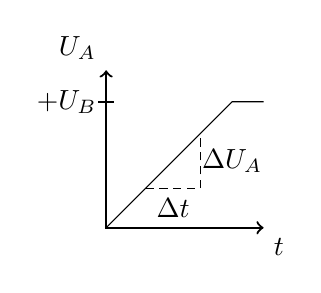
\begin{tikzpicture}
        \draw[thick,->] (-0.015,0) -- (2,0) node[anchor=north west] {$t$};
        \draw[thick,->] (0,0) -- (0,2) node[anchor=south east] {$U_{A}$};
        \draw (0,0) -- (1.6,1.6) -- (2,1.6);
        \draw[thick] (-0.1,1.6) -- (0.1,1.6);
        \draw (0,1.6) node[anchor=east] {$+U_B$};
        
        \draw[densely dashed] (0.5,0.5) -- (1.2,0.5) -- ++(0,0.7);  % Steigungsdreieck Linien
            \node at (1.6,0.85) {$\Delta U_A$};
            \node at (0.85,0.25) {$\Delta t$}; 
    \end{tikzpicture}} \\
    \hline
\end{tabular}}}{Schaltung des Beispielproblems mit einer Signalquelle auf der Eingangsseite und einer komplexen Last auf der Ausgangsseite \label{fig:Beispielproblem 1 Folien 2 Abbildung 1}} 
        }
    \end{frame}
    \begin{frame}
        \b{
            \frametitle{Prinzip der Gegenkopplung - Lösung des Beispielproblems (2)}
             \fu{\resizebox{0.8\textwidth}{!}{\begin{tabular}{|m{0.25\textwidth}|m{0.5\textwidth}|m{0.25\textwidth}|}
    \hline
    \begin{circuitikz}[scale=0.8, transform shape]
        \ctikzset{tripoles/en amp/input height=-0.45}
        \draw (0,0) node[en amp](E){};
        \node at ($(E) + (-1.2, 1.5)$) {\textbf{\LARGE A}}; % Label für den ersten OPV
        \draw (E.out) node[circ]{} node[right]{$U_A$};
        \draw (E.-) node[circ]{} node[left]{0V};
        \draw (E.+) node[circ]{} node[left]{1V};
        \draw (E.up) -- ++(0,0.5) node[anchor=south]{$+U_B$} node[circ] {};
        \draw (E.down) -- ++(0,-0.5) node[anchor=north]{$-U_B$} node[circ] {};
    \end{circuitikz} &
    \begin{circuitikz}[scale=0.8, transform shape]
        \ctikzset{tripoles/en amp/input height=-0.45}
        \draw (0,0) node[en amp](E){};
        \node at ($(E) + (-1.2, 1.5)$) {\textbf{\LARGE B}}; % Label für den ersten OPV im mittleren Bild
        \draw (E.out) node[circ]{} node[right]{$U_A$};
        \draw (E.-) node[circ]{} node[left]{0V} -- ++(0, -1) to[normal open switch] ++(2.38,0) -- ++(0,1.5);
        \draw (E.+) node[circ]{} node[left]{1V};
    
        \draw (4,0) node[en amp](E2){};
        \node at ($(E2) + (-1.2, 1.5)$) {\textbf{\LARGE C}}; % Label für den zweiten OPV im mittleren Bild
        \draw (E2.out) node[circ]{} node[right]{$U_A$};
        \draw (E2.-) node[circ]{} node[left]{0V} -- ++(0, -1) -- ++(2.38,0) -- ++(0,1.5);
        \draw (E2.+) node[circ]{} node[left]{1V};
    \end{circuitikz}
    \\
    \hline
    \multicolumn{1}{|c|}{
    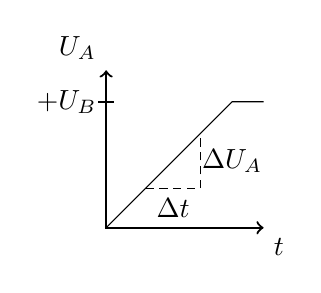
\begin{tikzpicture}
        \draw[thick,->] (-0.015,0) -- (2,0) node[anchor=north west] {$t$};
        \draw[thick,->] (0,0) -- (0,2) node[anchor=south east] {$U_{A}$};
        \draw (0,0) -- (1.6,1.6) -- (2,1.6);
        \draw[thick] (-0.1,1.6) -- (0.1,1.6);
        \draw (0,1.6) node[anchor=east] {$+U_B$};
        
        \draw[densely dashed] (0.5,0.5) -- (1.2,0.5) -- ++(0,0.7);  % Steigungsdreieck Linien
            \node at (1.6,0.85) {$\Delta U_A$};
            \node at (0.85,0.25) {$\Delta t$}; 
    \end{tikzpicture}} &
    \multicolumn{1}{c|}{
    \begin{tikzpicture}
        \draw[thick,->] (1.985,0) -- (4,0) node[anchor=north west] {$t$};
        \draw[thick,->] (2,0) -- (2,2) node[anchor=south east] {$U_{A}$};
        \draw (2,0) -- (3,0.5) -- (4,0.5);
        \draw[thick] (1.9,0.5) -- (2.1,0.5) node[anchor=east] {$1V$};
        \node at (0,1) {Slew rate: $\frac{\Delta U_A}{\Delta t}$};
    \end{tikzpicture}}
    \\
    \hline
    \end{tabular}}}{Schaltung des Beispielproblems mit einer Signalquelle auf der Eingangsseite und einer komplexen Last auf der Ausgangsseite \label{fig:Beispielproblem 1 Folien 2 Abbildung 2}} 
        }
    \end{frame}

%\speech{
% Beispiel 3.1: Teil 1: Entwicklung einer Verstärkerschaltung für Musiksignale.
% Bei der Entwicklung von Hi-Fi-Geräten müssen Verstärker an die Last (also den Lautsprecher) angepasst werden.
% Dazu wird ein Leistungsverstärker (d.h. eine Endstufe) benötigt. Eine solche Endstufe, die geeignet ist, das Signal eines Handys so zu verstärken, dass ein Lautsprecher damit betrieben werden kann soll hier aufgebaut werden.
% Ein vereinfachtes Ersatzschaltbild des Lautsprechers ist durch eine Induktivität mit einem in Reihe geschalteten Widerstand gegeben (siehe Abbildung \ref{fig:Beispielproblem 1}).
% Das Eingangsspannungsniveau ist 1~V und es soll ein 4~$\mathrm{\Omega}$ Lautsprecher betrieben werden (4~$\mathrm{\Omega}$ bedeutet, dass der Lautsprecher bei 1~kHz eine Impedanz von 4~$\Omega$ aufweist).
% Wie groß muss die Spannung am Ausgang des Verstärkers sein, damit der Lautsprecher bei 1~kHz 25 W aufnimmt? Wie kann hier vorgegangen werden, wenn eine Operationsverstärkerschaltung für die Lösung genutzt werden soll?
% Lösung: Zunächst muss dazu die Spannung berechnet werden, die der Verstärker ausgeben soll.
% U A = sqrt(P * R) = sqrt(25 W * 4 $\Omega$) = 10 V
% Wie kann nun mithilfe eines Operationsverstärkers der mit einem ? gekennzeichneten Teil der Schaltung ersetzt werden, um eine notwendige Verstärkung von 10 zu erreichen (siehe Abbildung \ref{fig:Beispielproblem 1})?
%} 

%\speech{
%Abbildung 3.1 zeigt eine Schaltung mit einer Signalquelle auf der Eingangsseite und einer komplexen Last auf der Ausgangsseite.  
%Die Signalquelle liefert eine Wechselspannung mit einer Amplitude von 1 Volt.  
%Das Signal wird an eine unbekannte Schaltung weitergeleitet, die durch ein Fragezeichen gekennzeichnet ist.  
%Diese Schaltung verstärkt oder verändert das Signal und gibt es an die Ausgangslast weiter.  
%
%Die Ausgangslast ist in einem gestrichelten Rechteck markiert und stellt ein Ersatzschaltbild für einen Lautsprecher dar.  
%Diese Last besteht aus einem Widerstand von 2 Ohm in Reihe mit einer Induktivität von 100 Millihenry.  
%Die Induktivität beeinflusst das Verhalten der Last in Abhängigkeit von der Frequenz des Eingangssignals.  
%
%Die Aufgabe besteht darin, den Verstärkungsfaktor der unbekannten Schaltung zu bestimmen.  
%Der Verstärkungsfaktor ist definiert als das Verhältnis der Ausgangsspannung U A zur Eingangsspannung U E.  
%Mathematisch ausgedrückt als V gleich U A geteilt durch U E.  
%
%Um den Verstärkungsfaktor zu berechnen, müssen die Eigenschaften der unbekannten Schaltung sowie die Auswirkungen der komplexen Last berücksichtigt werden.  
%}



\begin{frame}
    \s{\pagebreak
        Wie aus vorherigen Kapiteln bekannt ist, besitzen Operationsverstärker einen invertierenden und einen nicht-invertierenden Eingang. Existiert zwischen diesen beiden Eingängen eine Spannungsdifferenz, so verstärkt der Operationsverstärker diese Differenz um ein Vielfaches, bis die Spannung die maximale Ausgangsspannung des Operationsverstärkers erreicht (siehe A in Abbildung \ref{fig: Verschaltung Verstaerker}).
    Die Slew-Rate (zu deutsch: Anstiegsrate) gibt an, wie schnell dieser Anstieg geschehen kann. Wird die Ausgangsspannung nicht auf den Eingang zurückgeführt, steigt die Ausgangspannung, bis das Niveau der Versorgungsspannung erreicht wird. Eine solche Beschaltung des Verstärkers wird als Komperatorschaltung bezeichet.

    Dieses Verhalten ist für die meisten Anwendungen bei denen der Eingangsspannungssignal mit geringer Amplitude verstärkt werden soll, nicht erwünscht. 
    Stattdessen werden Operationsverstärker meistens in der sogenannten Gegenkopplung (B) betrieben, bei der der Ausgang auf den invertierenden Eingang zurückgeführt wird. 
    Der in (B) eingezeichnete Schalter sei zunächst geöffnet und der Operationsverstärker werde nicht mit Spannung versorgt. Zum Zeitpunkt 0 s wird der Schalter geschlossen und die Versorgungsspannung des Verstärkers eingeschaltet, wodurch die Rückführung des Ausgangssignals $U_{\textnormal{A}}$ aktiv wird (C). 
    Durch die Rückkopplung des Ausgangssignal wird so erreicht, dass die Spannung am invertierenden Eingang auf das Spannungsniveau der Ausgangsspannung angeglichen wird. 
    Die in (C) dargestellte Verstärkerschaltung hat die Verstärkung 1 und wird als Impedanzwandler bezeichnet, da der Verstärker in dieser Schaltungsart aufgrund seiner hohen Eingangsimpedanz verwendet werden kann, um eine Schaltung mit hochohmigem Eingang zu realisieren (dies ist beispielsweise bei Messschaltungen für Spannungsmessungen notwendig). 
    Für die Lösung des Anwendungsproblems ist diese Schaltung allerdings noch nicht geeignet, da eine Verstärkung von 5 gefordert ist. 
    Um diese zu erreichen werden in die Verstärkerschaltung nun zusätzlich Widerstände eingebaut (wie in (D) dargestellt ist)\footnote{Es lässt sich feststellen, dass sich für $R_2 = 0$ und $R_1 = \infty$ wieder die Schaltung des Impedanzwandlers ergibt. Der Impedanzwandler ist also ein Spezialfall des nicht-invertierenden Verstärkers.}.      
    }
    \b{\frametitle{Prinzip der Gegenkopplung - Lösung des Beispielproblems (2)}}
    \fu{
        \resizebox{\textwidth}{!}{\begin{tabular}{|m{0.25\textwidth}|m{0.45\textwidth}|m{0.3\textwidth}|}
    \hline
    \begin{circuitikz}[scale=0.8, transform shape]
        \ctikzset{tripoles/en amp/input height=-0.45}
        \draw (0,0) node[en amp](E){};
        \node at ($(E) + (-1.2, 1.5)$) {\textbf{\LARGE A}}; % Label für den ersten OPV
        \draw (E.out) node[circ]{} node[right]{$U_A$};
        \draw (E.-) node[circ]{} node[left]{0V};
        \draw (E.+) node[circ]{} node[left]{1V};
        \draw (E.up) -- ++(0,0.5) node[anchor=south]{$+U_B$} node[circ] {};
        \draw (E.down) -- ++(0,-0.5) node[anchor=north]{$-U_B$} node[circ] {};

    \end{circuitikz} &
    \begin{circuitikz}[scale=0.8, transform shape]
        \ctikzset{tripoles/en amp/input height=-0.45}
        \draw (0,0) node[en amp](E){};
        \node at ($(E) + (-1.2, 1.5)$) {\textbf{\LARGE B}}; % Label für den ersten OPV im mittleren Bild
        \draw (E.out) node[circ]{} node[right]{$U_A$};
        \draw (E.-) node[circ]{} node[left]{0V} -- ++(0, -1) to[normal open switch] ++(2.38,0) -- ++(0,1.5);
        \draw (E.+) node[circ]{} node[left]{1V};
    
        \draw (4,0) node[en amp](E2){};
        \node at ($(E2) + (-1.2, 1.5)$) {\textbf{\LARGE C}}; % Label für den zweiten OPV im mittleren Bild
        \draw (E2.out) node[circ]{} node[right]{$U_A$};
        \draw (E2.-) node[circ]{} node[left]{0V} -- ++(0, -1) -- ++(2.38,0) -- ++(0,1.5);
        \draw (E2.+) node[circ]{} node[left]{1V};
    \end{circuitikz} &
    \begin{circuitikz}[scale=0.8, transform shape]
        \ctikzset{tripoles/en amp/input height=-0.45,
        }
        \draw (0,0) node[en amp](E){};
        \node at ($(E) + (-1.2, 1.5)$) {\textbf{\LARGE D}}; % Label für den OPV im dritten Bild
        \draw (E.out) node[circ]{} -- ++(0.2,0) node[ocirc, right]{};
        \draw (E.-) -- ++(0, -1.3) node[circ] {} to[R, l=$R_2$] ++(2.38,0) -- ++(0,1.8);
        \draw (E.-) -- ++(0, -1.6) to[R, l_=$R_1$] ++(0, -1.2) -- ++(0,-0.2) -- ++(-0.2, 0) -- ++(0.4,0);
        \draw (E.+) node[circ]{} node[left]{};     
       
        % Spannungspfeil
        \draw[-{Triangle[width=3pt,length=4pt]}, color=spannung] ($(E.+) + (0, -0.1)$) -- ($(E.-) + (0, 0.1)$) node[midway, xshift=-30] {$U_{\text{Diff}}=0\,\text{V}$};
        \draw[-{Triangle[width=3pt,length=4pt]}, color=spannung] ($(E.out) + (0.26, -0.1)$) -- ($(E.out) + (0.26, -3.45)$) node[midway, xshift=10] {$U_A$};
        \draw[black] ($(E.out) + (0.26, -3.5)$) -- ++(-0.2, 0) -- ++(0.4,0);
        \draw[-{Triangle[width=3pt,length=4pt]}, color=spannung] (0.7,-2.1)-- ++(-1.5,0) node[midway, yshift=-10] {$U_{R2}$};
        \draw[-{Triangle[width=3pt,length=4pt]}, color=spannung] (-0.9,-2)-- ++(0,-1.5) node[midway, xshift=10] {$U_{R1}$};


        
        \node[red] at (0.9,-1.8) {\tikz \draw[red, -{Triangle[width=3pt,length=4pt]}] (0,0) -- (-0.01,0);};
        \node[above, color=red] at (0.9,-1.8)  {$I_{R2}$};

        \node[red] at ($(E.-)+(0,-1.5)$) {\tikz \draw[red, -{Triangle[width=3pt,length=4pt]}] (0,0) -- (0,-0.01);};
        \node[left, color=red] at ($(E.-)+(0,-1.4)$)  {$I_{R1}$};
    \end{circuitikz}
    \\
    \hline
    \multicolumn{1}{|c|}{
    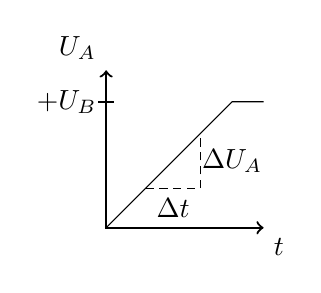
\begin{tikzpicture}
        \draw[thick,->] (-0.015,0) -- (2,0) node[anchor=north west] {$t$};
        \draw[thick,->] (0,0) -- (0,2) node[anchor=south east] {$U_{A}$};
        \draw (0,0) -- (1.6,1.6) -- (2,1.6);
        \draw[thick] (-0.1,1.6) -- (0.1,1.6);
        \draw (0,1.6) node[anchor=east] {$+U_B$};
        
        \draw[densely dashed] (0.5,0.5) -- (1.2,0.5) -- ++(0,0.7);  % Steigungsdreieck Linien
            \node at (1.6,0.85) {$\Delta U_A$};
            \node at (0.85,0.25) {$\Delta t$}; 
    \end{tikzpicture}} &
    \multicolumn{1}{c|}{
    \begin{tikzpicture}
        \draw[thick,->] (1.985,0) -- (4,0) node[anchor=north west] {$t$};
        \draw[thick,->] (2,0) -- (2,2) node[anchor=south east] {$U_{A}$};
        \draw (2,0) -- (3,0.5) -- (4,0.5);
        \draw[thick] (1.9,0.5) -- (2.1,0.5) node[anchor=east] {$1V$};
        \node at (0,1) {Slew rate: $\frac{\Delta U_A}{\Delta t}$};
    \end{tikzpicture}} &
    \multicolumn{1}{c|}{
    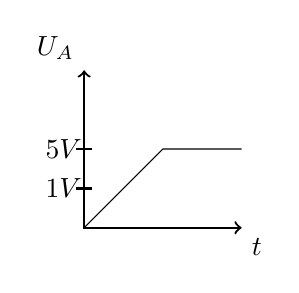
\begin{tikzpicture}
        \draw[thick,->] (-0.015,0) -- (2,0) node[anchor=north west] {$t$};
        \draw[thick,->] (0,0) -- (0,2) node[anchor=south east] {$U_{A}$};
        \draw (0,0) -- (1,1) -- (2,1);
        \draw[thick] (-0.1,1) -- (0.1,1) node[anchor=east] {$5V$};
        \draw[thick] (-0.1,0.5) -- (0.1,0.5) node[anchor=east] {$1V$};
    \end{tikzpicture}} \\
    \hline
    \end{tabular}}
        }{Verschaltung eines Verstärkers als Komperator (A), Impedanzwandler (C) und nicht-invertierender Verstärker (D)
        \label{fig: Verschaltung Verstaerker}}       
\end{frame}

%\speech {
%    Wie aus vorherigen Kapiteln bekannt ist, besitzen Operationsverstärker einen invertierenden und einen nicht-invertierenden Eingang. Existiert zwischen diesen beiden Eingängen eine Spannungsdifferenz, so verstärkt der Operationsverstärker diese Differenz um ein Vielfaches, bis die Spannung die maximale Ausgangsspannung des Operationsverstärkers erreicht (siehe A in Abbildung \ref{fig: Verschaltung Verstaerker}).
%    Die Slew-Rate (zu deutsch: Anstiegsrate) gibt an, wie schnell dieser Anstieg geschehen kann. Wird die Ausgangsspannung nicht auf den Eingang zurückgeführt, steigt die Ausgangspannung, bis das Niveau der Versorgungsspannung erreicht wird. Eine solche Beschaltung des Verstärkers wird als Komperatorschaltung bezeichet.
% Dieses Verhalten ist für die meisten Anwendungen bei denen der Eingangsspannungssignal mit geringer Amplitude verstärkt werden soll, nicht erwünscht.
% Stattdessen werden Operationsverstärker meistens in der sogenannten Gegenkopplung (B) betrieben, bei der der Ausgang auf den invertierenden Eingang zurückgeführt wird.
% Der in (B) eingezeichnete Schalter sei zunächst geöffnet und der Operationsverstärker werde nicht mit Spannung versorgt. Zum Zeitpunkt 0 s wird der Schalter geschlossen und die Versorgungsspannung des Verstärkers eingeschaltet, wodurch die Rückführung des Ausgangssignals $U_{\textnormal{A}}$ aktiv wird (C).
% Durch die Rückkopplung des Ausgangssignal wird so erreicht, dass die Spannung am invertierenden Eingang auf das Spannungsniveau der Ausgangsspannung angeglichen wird.
% Die in (C) dargestellte Verstärkerschaltung hat die Verstärkung 1 und wird als Impedanzwandler bezeichnet, da der Verstärker in dieser Schaltungsart aufgrund seiner hohen Eingangsimpedanz verwendet werden kann, um eine Schaltung mit hochohmigem Eingang zu realisieren (dies ist beispielsweise bei Messschaltungen für Spannungsmessungen notwendig).
% Für die Lösung des Anwendungsproblems ist diese Schaltung allerdings noch nicht geeignet, da eine Verstärkung von 5 gefordert ist.
% Um diese zu erreichen werden in die Verstärkerschaltung nun zusätzlich Widerstände eingebaut (wie in (D) dargestellt ist)\footnote{Es lässt sich feststellen, dass sich für $R_2 = 0$ und $R_1 = \infty$ wieder die Schaltung des Impedanzwandlers ergibt. Der Impedanzwandler ist also ein Spezialfall des nicht-invertierenden Verstärkers.}.
%}
%\speech{
%Abbildung 3.2 zeigt verschiedene Verschaltungen eines Operationsverstärkers und deren zugehörige Ausgangsverläufe.  
%Es sind vier verschiedene Konfigurationen dargestellt:  
%Ein Komparator, zwei Varianten eines Impedanzwandlers und ein nichtinvertierender Verstärker.  
%
%Im oberen Bereich der Abbildung sind die jeweiligen Schaltungen zu sehen.  
%Im unteren Bereich sind die entsprechenden Ausgangsdiagramme dargestellt, die den zeitlichen Verlauf der Ausgangsspannung U A zeigen.  
%
%Schaltung A zeigt einen Operationsverstärker als Komparator.  
%Der nichtinvertierende Eingang erhält eine konstante Spannung von 1 Volt.  
%Der invertierende Eingang ist auf 0 Volt gelegt.  
%Da die Eingangsspannung am nichtinvertierenden Eingang größer ist, springt die Ausgangsspannung auf den maximalen positiven Wert.  
%Das untere Diagramm zeigt den Ausgangsverlauf als sprunghafte Änderung.  
%
%Schaltung B und C zeigen einen Operationsverstärker als Impedanzwandler, auch Unity-Gain-Buffer genannt.  
%Hierbei wird die Eingangsspannung direkt am nichtinvertierenden Eingang angelegt.  
%Der Ausgang ist mit dem invertierenden Eingang verbunden, sodass eine Verstärkung von Eins entsteht.  
%Das untere Diagramm zeigt, dass die Ausgangsspannung genau der Eingangsspannung folgt.  
%
%Schaltung D zeigt einen nichtinvertierenden Verstärker.  
%Ein Spannungsteiler aus den Widerständen R1 und R2 bestimmt die Verstärkung.  
%Die Ausgangsspannung U A ist größer als die Eingangsspannung.  
%Das untere Diagramm zeigt eine Verstärkung des Signals, wobei die Ausgangsspannung von 1 Volt auf 5 Volt ansteigt.  
%
%Die Abbildung zeigt, wie sich unterschiedliche Verschaltungen auf die Ausgangsspannung auswirken.  
%}

\begin{frame}
    \s{
    \begin{bsp}{Teil 2: Entwicklung einer Verstärkerschaltung für Musiksignale}{Beispiel Verstaerkung 2}
        Im letzten Schritt muss ermittelt werden, wie die Widerstände in (D) gewählt werden müssen, damit sich eine Verstärkung von 5 ergibt. Dazu müssen zunächst die Maschengleichungen aufgestellt werden.
        Eine wichtige Annahme zur Aufstellung dieser Maschengleichung ist, dass davon ausgegangen wird, dass der Verstärker durch die Rückkopplung des Ausgangsignal die beiden Eingangssignale angleicht. 
        Hier darf also geschrieben werden \glqq Annahme: $U_{\textnormal{dif}}~=~0$~V\grqq{}. 
        Somit ergibt sich für den invertierenden Eingang $U_{\textnormal{E-}}~=~1$~V.
        Da weiterhin davon ausgegangen wird, dass kein Strom in die Eingänge hineinfließt gilt $I_{\textnormal{R1}}~=~I_{\textnormal{R2}}$.
        Die Maschengleichung lautet auf Grundlage dieser Annahmen
        \begin{equation}
            U_{\textnormal{A}} = U_{\textnormal{R1}} + U_{\textnormal{R2}} = U_{\textnormal{E}} + I_{\textnormal{R2}} \cdot R_{\textnormal{2}} = U_{\textnormal{E}} + \frac{U_{\textnormal{E}}}{R_{\textnormal{1}}} \cdot R_{\textnormal{2}} 
        \end{equation}

        Dadurch ergibt sich das Ein-Ausgangsverhalten im zeitbereich zu folgendem Ausdruck.
        \begin{equation}
            \frac{U_{\textnormal{A}}}{U_{\textnormal{E}}} = \underbrace{(1+\frac{R_2}{R_1})}_{V}
        \end{equation}
        

        Wird diese Gleichung nach $R_2/R_1$ gelöst, ergibt sich das Verhältnis der Widerstände für das oben beschriebene 
        Problem zu $R_2/R_1 = 9$. Die Widerstände sollten hier nicht zu groß gewählt werden, da dann der Ausgleichsstrom zwischen
        Ausgang und Eingang zu klein werden könnte. Das kann zu einem starken Rauschen am Verstärkerausgang führen. Übliche Widerstandswerte sind in der Regel den Beispielschaltungen des Datenblattes eines
        Operationsverstärkers zu entnehmen. In diesem Fall könnte z.B. $R_2=9~\textnormal{k}\Omega$ und $R_1=1~\textnormal{k}\Omega$ gewählt werden.
    \end{bsp} 

%\speech{1}{
%Beispiel 3.2: Teil 2: Entwicklung einer Verstärkerschaltung für Musiksignale.
%Im letzten Schritt muss ermittelt werden, wie die Widerstände in (D) gewählt werden müssen, damit sich eine Verstärkung von 5 ergibt. Dazu müssen zunächst die Maschengleichungen aufgestellt werden.
%Eine wichtige Annahme zur Aufstellung dieser Maschengleichung ist, dass davon ausgegangen wird, dass der Verstärker durch die Rückkopplung des Ausgangsignal die beiden Eingangssignale angleicht.
%Hier darf also geschrieben werden \glqq Annahme: $U_{\textnormal{dif}}~=~0$~V\grqq{}.
%Somit ergibt sich für den invertierenden Eingang $U_{\textnormal{E-}}~=~1$~V.
%Da weiterhin davon ausgegangen wird, dass kein Strom in die Eingänge hineinfließt gilt $I_{\textnormal{R1}}~=~I_{\textnormal{R2}}$.
%Die Maschengleichung lautet auf Grundlage dieser Annahmen
%\begin{equation}
%    U_{\textnormal{A}} = U_{\textnormal{R1}} + U_{\textnormal{R2}} = U_{\textnormal{E}} + I_{\textnormal{R2}} \cdot R_{\textnormal{2}} = U_{\textnormal{E}} + \frac{U_{\textnormal{E}}}{R_{\textnormal{1}}} \cdot R_{\textnormal{2}}
%\end{equation}
%Wird diese Gleichung nach $R_2/R_1$ gelöst, ergibt sich das Verhältnis der Widerstände für das oben beschriebene 
%Problem zu $R_2/R_1 = 9$. Die Widerstände sollten hier nicht zu groß gewählt werden, da dann der Ausgleichsstrom zwischen
%Ausgang und Eingang zu klein werden könnte. Das kann zu einem starken Rauschen am Verstärkerausgang führen. Übliche Widerstandswerte sind in der Regel den Beispielschaltungen des Datenblattes eines
%Operationsverstärkers zu entnehmen. In diesem Fall könnte z.B. $R_2=9~\textnormal{k}\Omega$ und $R_1=1~\textnormal{k}\Omega$ gewählt werden.
%}
        \par
        Ähnnlich wie für die oben dargestellte Schaltung lassen sich auch für alle weiteren Operationsverstärkerschaltungen Übertragungsfunktionen herleiten. Das soll hier allerdings nicht gezeigt werden.
        Weitere Übertragungsfuktionen für einige ausgewählte Operationsverstärkergrundschaltungen können Tabelle \ref{tab:Grundschaltungen} entnommen werden. 
        In dieser Tabelle sind die die Schaltungen, die Bodediagramme mit Phasengang (rot) und Amplitudengang (blau) und die Übertragungsfunktionen angegeben. 
        Nachdem nun die Beschaltung von Verstärkern vorgestellt wurde, soll im Folgenden Kapitel nun noch eine wichtige Eigenschaft von Verstärkerschaltungen thematisiert werden, die sich aus den genutzen Verstärkerbausteinen und der äußeren Verschaltung ergibt: Die Stabilität der Verstärkerschaltung.
        
%\speech {1}{
% Ähnlich wie für die oben dargestellte Schaltung lassen sich auch für alle weiteren Operationsverstärkerschaltungen Übertragungsfunktionen herleiten. Das soll hier allerdings nicht gezeigt werden.
%    Weitere Übertragungsfuktionen für einige ausgewählte Operationsverstärkergrundschaltungen können Tabelle \ref{tab:Grundschaltungen} entnommen werden.
%    In dieser Tabelle sind die die Schaltungen, die Bodediagramme mit Phasengang (rot) und Amplitudengang (blau) und die Übertragungsfunktionen angegeben.
%    Nachdem nun die Beschaltung von Verstärkern vorgestellt wurde, soll im Folgenden Kapitel nun noch eine wichtige Eigenschaft von Verstärkerschaltungen thematisiert werden, die sich aus den genutzen Verstärkerbausteinen und der äußeren Verschaltung ergibt: Die Stabilität der Verstärkerschaltung.   
%}
        
%\speech{
%Tabelle 3.1 zeigt verschiedene Grundschaltungen mit Operationsverstärkern.  
%Die Tabelle ist in drei Spalten unterteilt.  
%Die erste Spalte zeigt die Schaltung, die zweite Spalte enthält den Frequenzgang und die Gleichung,  
%und die dritte Spalte gibt eine Erklärung mit den wichtigsten Eigenschaften.  
%
%Erste Zeile: Nichtinvertierender Verstärker.  
%Die Ausgangsspannung ist phasengleich mit der Eingangsspannung.  
%Die Verstärkung ist eins plus das Verhältnis von R2 zu R1.  
%Der Verstärker hat einen sehr hohen Eingangswiderstand und einen niedrigen Ausgangswiderstand.  
%Anwendungsbeispiel ist ein Impedanzwandler.  
%
%Zweite Zeile: Invertierender Verstärker.  
%Die Ausgangsspannung ist um 180 Grad phasenverschoben zur Eingangsspannung.  
%Die Verstärkung ist das Verhältnis von R2 zu R1.  
%Der Widerstand R1 bestimmt den Eingangswiderstand.  
%Anwendungsbeispiel ist ein aktiver Spannungsteiler für hohe Spannungen.  
%
%Dritte Zeile: Komparator.  
%Die Ausgangsspannung ist entweder hoch oder niedrig, je nach Vergleich der Eingänge.  
%Wenn die nichtinvertierende Spannung größer ist als die invertierende Spannung,  
%geht die Ausgangsspannung auf den oberen Versorgungswert.  
%Andernfalls geht sie auf den unteren Versorgungswert.  
%Wird verwendet in Zweipunktreglern und Analog-Digital-Wandlern.  
%
%Vierte Zeile: Summierer.  
%Der Summierer basiert auf einem invertierenden Verstärker.  
%Die Ausgangsspannung ist eine gewichtete Summe mehrerer Eingangsspannungen.  
%Wird verwendet in Analogrechnern und zur Mischung von Signalen.  
%
%Fünfte Zeile: Subtrahierer.  
%Diese Schaltung bildet die Differenz zwischen zwei Eingangsspannungen.  
%Wenn alle Widerstände gleich sind, entspricht die Ausgangsspannung genau der Differenz der Eingänge.  
%Diese Schaltung wird als Differenzverstärker verwendet.  
%
%Sechste Zeile: Integrierer.  
%Der Integrierer summiert die Eingangsspannung über die Zeit.  
%Die Ausgangsspannung entspricht dem negativen Integral des Eingangssignals.  
%Wird als aktiver Tiefpassfilter verwendet.  
%
%Siebte Zeile: Differenzierer.  
%Der Differenzierer bildet die Ableitung des Eingangssignals.  
%Die Ausgangsspannung ist proportional zur zeitlichen Änderung der Eingangsspannung.  
%Wird als Hochpassfilter eingesetzt, zeigt in der Praxis aber oft ein Bandpassverhalten.  
%
%Diese Tabelle gibt einen Überblick über wichtige Operationsverstärkerschaltungen  
%und ihre typischen Anwendungen in der Signalverarbeitung.  
%}



        \begin{block}{}
            \begin{table}[ht]
    \caption{Ausgewählte Operationsverstärker-Grundschaltungen}
    \label{tab:Grundschaltungen}
    \begin{tabular}{|m{0.24\textwidth}|m{0.405\textwidth}|m{0.33\textwidth}|}
    \hline
    Schaltung & Frequenzgang und Gleichung & Erläuterung und Eigenschaften\\ % Neue Zeile mit Text
    \hline
    \vspace{0.5cm}
    \centering
    \begin{circuitikz}[scale=0.7, transform shape]
    \ctikzset{
         resistors/scale=0.8,              
         tripoles/en amp/height=1.4, % Höhe des OPV             
         tripoles/en amp/width=1.4,   % Breite des OPV
         tripoles/en amp/input height=-0.45
    }
    \vspace{1ex}
    \draw (2,-0.1) node[en amp] (opamp) {}
    (opamp.+) --++ (-0.5,0) node[ocirc, label=left:$U_E$] (eingang) {} 
    (opamp.out) --++ (0.5,0) node[ocirc, label=right:$U_A$] {}
    (opamp.-) -- ++(0, -1.5) to[R, l=$R_1$] ++(0, -1) node[ground] {}
    (opamp.out) node[circ] {} -- ++(0,-1.5) to[R, l=$R_2$] ++(-1.95,0) node[circ] (feedback) {};
\end{circuitikz}

 & \begin{tikzpicture}[scale=1, transform shape]
    \begin{axis}[
    width=4.5cm, % Breite des Graphen
    height=3.5cm, % Höhe des Graphen
    xmin=0, xmax=10,
    ymin=0, ymax=120,
    axis lines=left,
    axis on top=true,
    domain=0:10,
    xtick=\empty,
    ytick=\empty,
    ylabel style={rotate=270, anchor=east, yshift=1cm}, % Position der Beschriftung oben links, horizontal
     ylabel={\it V}, % Hier die gewünschte Beschriftung einfügen
    xlabel={f[Hz]},
    clip mode=individual % Verhindert das Abschneiden von Elementen
    ]
    \path[draw=none] (axis cs:-4, 0) rectangle (axis cs:16.6,120);
    
    
    \coordinate (xaxis) at (axis description cs:15.5,0); % Verwendet die relative Positionierung für x-Achse
    
    \addplot+[mark=none, thick, blue] coordinates {(0,80) (10,80)};
    % Adding the left-side label
    \node[anchor=east] at (axis cs:0,80) {$1 + \frac{R_2}{R_1}$};
    \end{axis}
    \begin{axis}[
    width=4.5cm, % Breite des Graphen
    height=3.5cm, % Höhe des Graphen
    xmin=0, xmax=10,
    ymin=-180, ymax=180,
    axis y line*=right,
    axis x line=none,
    ytick=\empty,
    ylabel={$\varphi$},
    ylabel style={rotate=270, anchor=west, yshift=0.8cm},
    clip mode=individual, % Verhindert das Abschneiden von Elementen
    after end axis/.code={
        \draw[->] (axis cs:10,180) -- (axis cs:10,190);
    }
    ]
    \addplot+[mark=none, thick, red] coordinates {(0,0) (10,0)};
    \node[anchor=west] at (axis cs:10,0) {$0^\circ$};
    \end{axis}
    \end{tikzpicture}
\vspace{1ex}
\[
U_{\textnormal{A}} = \left(1+\frac{R_2}{R_1}\right) U_{\textnormal{E}}
\]
    &
    \textbf{Nicht-invertierender Verstärker}
\begin{itemize}
    \item Phasengleiches Ausgangs-\linebreak signal
    \item Sehr hochohmiger Eingangswiderstand
    \item Niederohmiger Ausgangs-\linebreak widerstand
    \item Anwendungen: z.B. Impedanzwandler
\end{itemize} \\
    \hline
    \centering
    \input{Tikz/InvertierenderVerstaerker.tex}
     & 
    \begin{center}
        \input{Tikz/FrequenzgangInvertierenderVerstaerker.tex}
\end{center}
\vspace{1ex}
\[
    U_{\textnormal{A}} = \frac{R_2}{R_1} U_{\textnormal{E}}
\]
    &
    \textbf{Invertierender Verstärker}
\begin{itemize}
    \item -180$^\circ$ Phasenverschiebung zwischen Ein- zu Ausgang
    \item $R_1$ bestimmt den Eingangswiderstand
    \item Niederohmiger Ausgangs-\linebreak widerstand
    \item Anwendungen: \linebreak z.B. Aktiver Spannungsteiler zum Messen hoher Spannungen, wenn $R_1 > R_2$
\end{itemize}
\\ % Zweite Zeile
    \hline
    \centering
    \begin{circuitikz}[scale=0.7, transform shape]
    \ctikzset{
          resistors/scale=0.8,              
          tripoles/en amp/height=1.4, % Höhe des OPV             
          tripoles/en amp/width=1.4,   % Breite des OPV
         tripoles/en amp/input height=0.45
     }
     \draw
     (0,0) node[en amp] (opamp) {}
     (opamp.-)  to[short, o-] ++(0,0) node[left] {$U_{E-}$}
      (opamp.+) to[short, o-] ++(0,0) node[left] {$U_{E+}$}
     (opamp.out) to[short, -o] ++(0,0) node[right] {$U_{A}$};
 \end{circuitikz}
    & 
    \begin{center}
               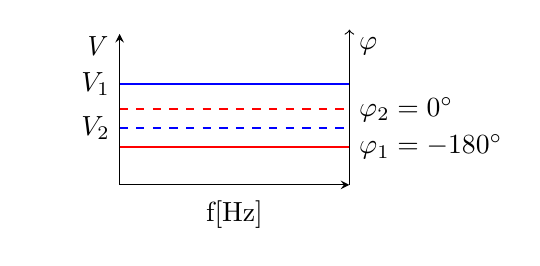
\begin{tikzpicture}[scale=1, transform shape]
    \begin{axis}[
        width=4.5cm, % Breite des Graphen
        height=3.5cm, % Höhe des Graphen
        xmin=0, xmax=10,
        ymin=0, ymax=120,
        axis lines=left,
        axis on top=true,
        domain=0:10,
        xtick=\empty,
        ytick=\empty,
        ylabel style={rotate=270, anchor=east, yshift=0.8cm},
         ylabel={\it V},
        xlabel={f[Hz]},
        clip mode=individual % Verhindert das Abschneiden von Elementen
        ]
        \path[draw=none] (axis cs:-4, 0) rectangle (axis cs:16.6,120);

        \addplot+[mark=none, thick, blue] coordinates {(0,80) (10,80)};
        \addplot+[mark=none, thick, blue, dashed] coordinates {(0,45) (10,45)};
        % Adding the left-side label
        \node[anchor=east] at (axis cs:0,80) {$V_1$};
        \node[anchor=east] at (axis cs:0,45) {$V_2$};
    \end{axis}
    \begin{axis}[
        width=4.5cm, % Breite des Graphen
        height=3.5cm, % Höhe des Graphen
        xmin=0, xmax=10,
        ymin=-180, ymax=180,
        axis y line*=right,
        axis x line=none,
        ytick=\empty,
        ylabel={$\varphi$},
        ylabel style={rotate=270, anchor=west, yshift=0.8cm},
        clip mode=individual, % Verhindert das Abschneiden von Elementen
        after end axis/.code={
            \draw[->] (axis cs:10,180) -- (axis cs:10,190);
        }
        ]
        \addplot+[mark=none, thick, red, dashed] coordinates {(0,0) (10,0)};
        \addplot+[mark=none, thick, red] coordinates {(0,-90) (10,-90)};
        \node[anchor=west] at (axis cs:10,0) {$\varphi_2 = 0^\circ$};
        \node[anchor=west] at (axis cs:10,-90) {$\varphi_1 = -180^\circ$};
    \end{axis}
    \end{tikzpicture}
\[
V_1: U_{\textnormal{E+}} > U_{\textnormal{E-}} \Rightarrow U_{\textnormal{A}} \approx +U_{\textnormal{B}}
\]
\[
V_2: U_{\textnormal{E+}} < U_{\textnormal{E-}} \Rightarrow U_{\textnormal{A}} \approx -U_{\textnormal{B}}
\]
\end{center}
    &\textbf{Komparator}\newline
    Einsatz in Zweipunktreglern und Analog-Digital-Wandlern
\\ % Dritte Zeile
    \hline

    

\centering
\begin{circuitikz}[scale=0.7, transform shape]
    \ctikzset{
        resistors/scale=0.8,              
        tripoles/en amp/height=1.4, % Höhe des OPV             
        tripoles/en amp/width=1.4,   % Breite des OPV
        tripoles/en amp/input height=0.45
    }
    \draw
    (0,0) node[en amp] (opamp) {}
    % R2 mit korrigiertem Strompfeil
    (opamp.-) -- ++(-0.4,0) node[circ] {} to[R, l_=$R_2$] ++(-1.5,0) node[ocirc] (R2left) {}
    % R1 mit korrigiertem Strompfeil
    (opamp.-) -- ++(-0.4,0) --++(0,1) to[R, l_=$R_1$] ++(-1.5,0) node[ocirc] (R1left) {}
    % Erdung
    (opamp.+) -- ++(0,0) node[ground] {}
    % Ausgang
    (opamp.out) to[short, *-o] ++(0,0) node[right] {$U_{A}$}
    % R3 mit Strompfeil
    (opamp.out) -- ++(0,1.5) to[R, l_=$R_3$] ++(-2,0) -- ++(0,-1.05) node[circ] {}
    % Spannungen U_E1 und U_E2 an den Knoten links von R1 und R2
    (R1left) node[left] {$U_{E1}$}
    (R2left) node[left] {$U_{E2}$};
\end{circuitikz}

    &
    \begin{center}
    \input{Tikz/FrequenzgangSummierer.tex}
\end{center}
\vspace{1ex}
\[
\begin{aligned}
    U_{\textnormal{A}} = \underbrace{\frac{R_3} {R_1}}_{V_1} \cdot U_{\textnormal{E1}} + \underbrace{\frac{R_3} {R_2}}_{V_2} \cdot U_{\textnormal{E2}}
\end{aligned}
\]
    & 
    \textbf{Summierer}\newline
    Der Summierer basiert auf dem invertierenden Verstärker und findet Verwendung in Analogrechnern und beim Mischen von Spannungssignalen
    \\ % Vierte Zeile
    \hline
    
    \end{tabular}
\end{table}


\newpage












\begin{table}[ht]
    \begin{tabular}{|m{0.23\textwidth}|m{0.44\textwidth}|m{0.33\textwidth}|}
     \hline 
    Schaltung & Frequenzgang und Gleichung & Erläuterung und Eigenschaften \\ % Neue Zeile mit Text
    \hline
    \begin{circuitikz}[scale=0.7, transform shape]
    \ctikzset{
          resistors/scale=0.8,              
          tripoles/en amp/height=1.4, % Höhe des OPV             
          tripoles/en amp/width=1.4,   % Breite des OPV
         tripoles/en amp/input height=0.45
     }
     \draw
     (0,0) node[en amp] (opamp) {}
     (opamp.-) to[R, l_=$R_1$, o-] ++(-1.2,0) to[short, o-] ++(0,0) node[left] {$U_{E1}$}
     (opamp.+) node[circ] {} to[R,  l_=$R_4$] ++(0,-1.5) node[ground] {}
     (opamp.-) node[circ] {} -- ++(0,1) to[R, l=$R_2$] ++(1.9,0) -| (opamp.out)
     (opamp.out) to[short, *-o] ++(0.2,0) node[right] {$U_{A}$}
     (opamp.+) to[R, l_=$R_3$, *-] ++(-1.2,0) to[short, o-] ++(0,0) node[left] {$U_{E2}$};
 \end{circuitikz}
      &
      \begin{center}
      \input{Tikz/FrequenzgangSubtrahierer.tex}
 \end{center}
 \vspace{1ex}
 \[
 \begin{aligned}
    {U_A} = {U_{{\textnormal{E2}}}} \cdot \underbrace{ \frac{R_1 + R_2}{R_1} \cdot \frac{R_4}{R_3 + R_4}}_{V_2} - U_{\textnormal{E1}} \cdot \underbrace{\frac{R_2}{R_1}}_{V_1}
\end{aligned}
 \]
     &
     \textbf{Subtrahierer}\newline
     Wenn alle Widerstände gleich groß sind, wird die Differenz der Signale $U_{E1}$ und $U_{E2}$ gebildet, weswegen diese Schaltung als Differenzverstärker bezeichnet wird
 \\ % Fünfte Zeile
     \hline

    \begin{circuitikz}[scale=0.7, transform shape]
    \ctikzset{
          resistors/scale=0.8,              
          tripoles/en amp/height=1.4, % Höhe des OPV             
          tripoles/en amp/width=1.4,   % Breite des OPV
         capacitors/scale=0.5,
         tripoles/en amp/input height=0.45
     }
     \vspace{1ex}
     \draw (2,0) node[en amp] (opamp) {}
     (opamp.+) --++ (-0.5,0) node[ground] {} 
     (opamp.out) --++ (0.2,0) node[ocirc, label=right:$U_A$] {}
     (opamp.-) -- ++(0, 0) to[R, l_=$R_1$] ++(-1.2, 0) node[ocirc, label=left:$U_E$] {}
     
     (opamp.out) node[circ] {} -- ++(0,1.5) to[C, l_=$C_1$, *-] ++(-1.9,0) node[circ]{}
     (opamp.out) node[circ] {} -- ++(0,2.8) to[R, l_=$R_2$] ++(-1.9,0) -- ++(0, -2.35) node[circ] {};
     \end{circuitikz}
     & 
     \begin{center}
    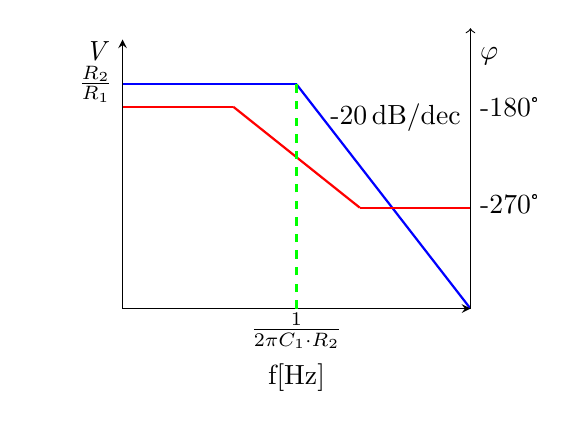
\begin{tikzpicture}[scale=1, transform shape]
    \begin{axis}[
       width=6cm, % Breite des Graphen
       height=5cm, % Höhe des Graphen
        xmin=0, xmax=11,
        ymin=0, ymax=1.2,
        axis lines=center,
        axis on top=true,
        domain=0:10,
        xtick=\empty,
        ytick=\empty,
        ylabel style={xshift=-0.6cm, yshift=0.1cm },
       ylabel={\it V},
       xlabel style={yshift=-0.4cm },
        xlabel={f[Hz]},
        clip mode=individual, % Verhindert das Abschneiden von Elementen
        xlabel style={at={(axis description cs:0.5,-0.05)},anchor=north}
        ]

        \path[draw=none] (axis cs:-3, 0) rectangle (axis cs:13,1);



        \addplot+[mark=none, thick, blue] coordinates {(0,1) (5.5,1)};
        \addplot+[mark=none, thick, blue] coordinates {(5.5,1) (11,0)};
        \node[anchor=east] at (axis cs:0,1) {$\frac{R_2}{R_1}$};
       \node[anchor=east] at (axis cs:11,0.85) {-20\,\text{dB/dec}};
    \end{axis}
    
    \begin{axis}[
       width=6cm, % Breite des Graphen
       height=5cm, % Höhe des Graphen
       xmin=0, xmax=11,
       ymin=0, ymax=240, 
       axis y line*=right,
       axis x line=none,
       ylabel={$\varphi$},
       ylabel style={rotate=270, anchor=west, yshift=1.5cm},
       xtick=\empty,
       ytick=\empty,
       clip mode=individual, % Verhindert das Abschneiden von Elementen
       after end axis/.code={
           \draw[->] (axis cs:11,240) -- (axis cs:11,250);
       }
        ]
        \addplot+[mark=none, thick, red] coordinates {(0,180) (3.5,180)};
        \addplot+[mark=none, thick, red] coordinates {(3.5,180) (7.5,90)};
        \addplot+[mark=none, thick, red] coordinates {(7.5,90) (11,90)};
        \addplot+[mark=none,dashed, thick, green] coordinates {(5.5,0) (5.5,200)};
        \node[] at (axis cs:5.5,-20) {$\frac{1}{2 \pi C_1 \cdot R_2}$};
        \node[anchor=west] at (axis cs:11,180) {-180°};
        \node[anchor=west] at (axis cs:11,93) {-270°};
    \end{axis}
    \end{tikzpicture}
     \[
     U_A(t) = - \frac{R_2}{R_1} U_{\textnormal{E}}(t) - \int_0^t \frac{U_{\textnormal{E}}(t)}{R_1 C_1} \, dt
     \]
     \end{center} 
     &
    \textbf{Integrierer/Integrator}\newline
    \begin{itemize}
        \item Nimmt eine Integration des Eingangssignals vor
        \item Wird als aktives Tiefpassfilter verwendet
    \end{itemize}
      \\ 
      \hline
    \input{Tikz/Differenzierer.tex}
    &
    \begin{center}
    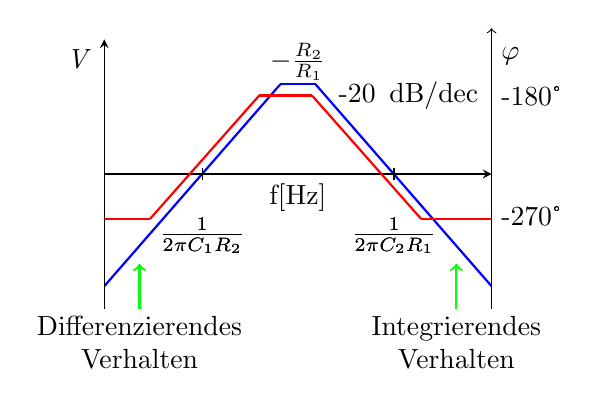
\begin{tikzpicture}[scale=1, transform shape]
    \begin{axis}[
        width=6.5cm, % Breite des Graphen
        height=5cm, % Höhe des Graphen
        xmin=0, xmax=11,
        ymin=-1.2, ymax=1.2,
        axis lines=center,
        axis on top=true,
        domain=0:10,
        clip mode=individual, % Verhindert das Abschneiden von Elementen
        xtick=\empty,
        ytick=\empty,
        ylabel style={xshift=-0.6cm},
        ylabel={\it V},
        xlabel={f[Hz]},
        xlabel style={at={(axis description cs:0.5,0.5)},anchor=north}
        ]
        \path[draw=none] (axis cs:-2, 0) rectangle (axis cs:13,1); \path[draw=none] (axis cs:-2, 0) rectangle (axis cs:13,1);


        \addplot+[mark=none, thick, blue] coordinates {(0,-1) (5,0.8)};
        \addplot+[mark=none, thick, blue] coordinates {(5,0.8) (6,0.8)};
        \addplot+[mark=none, thick, blue] coordinates {(6,0.8) (11,-1)};
        \node[anchor=north] at (axis cs:5.5,1.25) {$-\frac{R_2}{R_1}$};
        \addplot+[only marks, mark=|, black] coordinates {(2.78,0)} node[anchor=south] at (axis cs:2.78,-0.8) {$\frac{1}{2 \pi C_1 R_2}$};
        \addplot+[only marks, mark=|, black] coordinates {(8.23,0)} node[anchor=south] at (axis cs:8.23,-0.8) {$\frac{1}{2\pi C_2 R_1}$};
        \node[anchor=east] at (axis cs:10.9,0.7) {-20\, \text{dB/dec}};
        \addplot+[only marks, mark=|, black] coordinates {(2.78,0)} node[anchor=south] at (axis cs:2.78,-0.8) {$\frac{1}{2 \pi C_1 R_2}$};
        \addplot+[only marks, mark=|, black] coordinates {(8.23,0)} node[anchor=south] at (axis cs:8.23,-0.8) {$\frac{1}{2\pi C_2 R_1}$};
        \draw[->, thick, green] (axis cs:1,-1.2) -- (axis cs:1,-0.8);
        \node[align=center, black] at (axis cs:1,-1.5) {Differenzierendes\\ Verhalten};
        
        \draw[->, thick, green] (axis cs:10,-1.2) -- (axis cs:10,-0.8);
        \node[align=center, black] at (axis cs:10,-1.5) {Integrierendes\\ Verhalten};
        
    \end{axis}
    
    \begin{axis}[
        width=6.5cm, % Breite des Graphen
        height=5cm, % Höhe des Graphen
        xmin=0, xmax=11,
        ymin=0, ymax=240, 
        axis y line*=right,
        axis x line=none,
        ylabel={$\varphi$},
        ylabel style={rotate=270, anchor=west, yshift=1.5cm},
        xtick=\empty,
        ytick=\empty,
        clip mode=individual, % Verhindert das Abschneiden von Elementen
        after end axis/.code={
            \draw[->] (axis cs:11,240) -- (axis cs:11,250);
        }
        ]
        \addplot+[mark=none, thick, red] coordinates {(0,80) (1.3,80)};
        \addplot+[mark=none, thick, red] coordinates {(1.3,80) (4.4,190)};
        \addplot+[mark=none, thick, red] coordinates {(4.4,190) (5.9,190)};
        \addplot+[mark=none, thick, red] coordinates {(5.9,190) (9,80)};
        \addplot+[mark=none, thick, red] coordinates {(9,80) (11,80)};
        \node[anchor=west] at (axis cs:11,82.5) {-270°};
        \node[anchor=west] at (axis cs:11,190) {-180°};
       
    \end{axis}

    
    \end{tikzpicture}
    \begin{multline*}
        U_A = - \frac{R_2}{R_1} U_{\textnormal{E}}(t) \\
        - \int_0^t \frac{1}{R_1 C_1} U_{\textnormal{E}}(t) \, dt 
        - R_2 C_2\frac{dU_{\textnormal{E}}(t)}{dt}
    \end{multline*}
    \end{center} 
    & 
    \textbf{Differenzierer}\newline
    \begin{itemize}
        \item Nimmt eine Integration des Eingangssignals vor
        \item Wird als aktives Hochpassfilter verwendet (zeigt in der Realität meist Bandpassverhalten, wie hier dargestellt)
    \end{itemize}
    \\
    \hline
\end{tabular}
\end{table}






\newpage
    \begin{table}[ht]
        \begin{tabular}{|m{0.285\textwidth}|m{0.395\textwidth}|m{0.33\textwidth}|}
            \hline 
    Schaltung & Frequenzgang und Gleichung & Erläuterung und Eigenschaften \\ % Neue Zeile mit Text
    \hline
    \begin{circuitikz}[scale=0.7, transform shape]
    \ctikzset{
          resistors/scale=0.8,              
          tripoles/en amp/height=1.4, % Höhe des OPV             
          tripoles/en amp/width=1.4,   % Breite des OPV
         diodes/scale=0.8,
         tripoles/en amp/input height=0.45
     }
     \draw
     (0,0) node[en amp] (opamp) {}
     (opamp.-) to[R, l_=$R_1$, *-] ++(-1.2,0) to[short, o-] ++(0,0) node[left] {$U_E$}
     (opamp.+) -- ++(0,0) node[ground] {}
     (opamp.-) |- ++(0,1.5) to[D, l^=$D_1$] ++(2,0) -| (opamp.out)
     (opamp.out) to[short, *-o] ++(0.2,0) node[right] {$U_{A}$};
 \end{circuitikz}
    &
    \begin{center}
    \[
    U_{\textnormal{A}} =-U_{\textnormal{T}}\cdot \ln{\left(\frac{U_{\textnormal{E}}}{R_1\cdot I_S}\right)}
    \]
        \[
            U_{\textnormal{T}} = \frac{k_{\textnormal{B}} \cdot T}{e}
            \]
            
            \(e = \text{Elementarladung}\)
            
            \(k_{\textnormal{B}} = \text{Boltzmannkonstante}\)
            
            \(I_{\textnormal{s}} = \text{Sperrstrom der Diode}\)
    \end{center} 
    & 
    \textbf{Logarithmierer}\newline
    Bildet den natürlichen Logarithmus des Eingangssignals
    \\
    \hline
    \input{Tikz/Potenzierer.tex}
    &
    \begin{center}
    \[
    U_{\textnormal{A}} =-R_1\cdot I_{\textnormal{S}} \cdot e^{\frac{U_{\textnormal{E}}}{U_{\textnormal{T}}}}
    \]
    \end{center} 
    & 
    \textbf{Potenzierer}\newline
    Besitzt einen e-funktionalen Zusammenhang zwischen Ein- und Ausgangsspannung
    \\
    \hline
    \begin{circuitikz}[scale=0.6, transform shape]
    \ctikzset{
         resistors/scale=0.8,              
         tripoles/en amp/height=1.4, % Höhe des OPV             
         tripoles/en amp/width=1.4   % Breite des OPV
    }
    \draw 
    % Erster OPV mit input height=-0.45
    (2,-4.5) node[en amp, noinv input down] (opamp1) {}
    (opamp1.+) --++ (-0.5,0) node[ocirc, label=left:$U_{E2}$] (eingang1) {};
    
   \draw (2,0) node[en amp, noinv input up] (opamp2) {}
    (opamp2.+) --++ (-0.5,0) node[ocirc, label=left:$U_{E1}$] (eingang2) {}
    (opamp1.-)  to[R=$R_g$] (opamp2.-);

   % Dritter OPV mit angepasstem Eingangsabstand
    \ctikzset{tripoles/en amp/input height=0.55} % Anpassung nur für diesen OPV
    \draw (6,-2.25) node[en amp] (opamp3) {}
    (opamp3.-) -- ++(-0.5,0) to[R=$R_1$] ++(-1.5,0) to[R=$R_2$] ++(-2,0) node[circ]{}
    (opamp3.+) -- ++(-0.5,0) to[R=$R_3$] ++(-1.5,0) to[R=$R_4$] ++(-2,0) node[circ]{}
    (opamp2.out) -- ++(0,-1.72) node[circ]{}
    (opamp1.out) -- ++(0,1.72) node[circ]{}
    (opamp3.out) node[circ, label=below:{$U_A$}]{} -- ++(0, 2) to[R=$R_5$] ++(-2,0) -- ++(0, -1.45)node[circ]{};

\end{circuitikz}
     &
         \begin{center}
   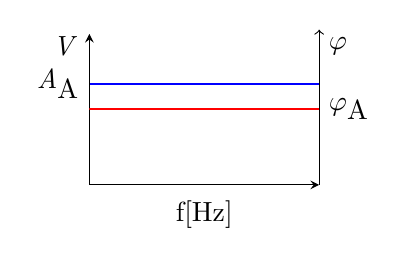
\begin{tikzpicture}[scale=1, transform shape]
    \begin{axis}[
        width=4.5cm, % Breite des Graphen
        height=3.5cm, % Höhe des Graphen
        xmin=0, xmax=10,
        ymin=0, ymax=120,
        axis lines=left,
        axis on top=true,
        domain=0:10,
        xtick=\empty,
        ytick=\empty,
        ylabel style={rotate=270, anchor=east, yshift=0.8cm}, % Position der Beschriftung oben links, horizontal
         ylabel={\it V}, % Hier die gewünschte Beschriftung einfügen
        xlabel={f[Hz]},
        clip mode=individual % Verhindert das Abschneiden von Elementen
        ]
        \addplot+[mark=none, thick, blue] coordinates {(0,80) (10,80)};
        % Adding the left-side label
        \node[anchor=east] at (axis cs:0,80) {$\mathit{A}_{\textnormal{A}}$};
    \end{axis}
    \begin{axis}[
        width=4.5cm, % Breite des Graphen
        height=3.5cm, % Höhe des Graphen
        xmin=0, xmax=10,
        ymin=-180, ymax=180,
        axis y line*=right,
        axis x line=none,
        ytick=\empty,
        ylabel={$\varphi$},
        ylabel style={rotate=270, anchor=west, yshift=0.8cm},
        clip mode=individual, % Verhindert das Abschneiden von Elementen
        after end axis/.code={
            \draw[->] (axis cs:10,180) -- (axis cs:10,190);
        }
        ]
        \addplot+[mark=none, thick, red] coordinates {(0,0) (10,0)};
        \node[anchor=west] at (axis cs:10,0) {$\varphi_{\textnormal{A}}$};
    \end{axis}
    \end{tikzpicture}
\end{center}

\vspace{1ex}
\[
\mathit{a_i} : \text{Amplitude Eingangsspannung i}
\]
\[
\mathit{\varphi_i} : \text{Phase Eingangsspannung i}
\]
\[
\mathit{A}_{A} = \sqrt{a_1^2 + a_2^2 + 2a_1a_2 \cos(\varphi_1 - \varphi_2)}
\]
\[
\mathit{\tan}(\varphi_A) = \frac{a_1 \mathit{\sin}(\varphi_1) + a_2 \mathit{\sin}(\varphi_2)}{a_1 \mathit{\cos}(\varphi_1) + a_2 \mathit{\cos}(\varphi_2)}
\]
\[
    \text{Wenn} : R_2 = R_4 = R
\]
\[
    U_{\textnormal{A}} = (1+ \frac{2R} {R_{\textnormal{g}}}) \cdot \frac{R_3} {R_2} (U_{\textnormal{E2}}-U_{\textnormal{E1}})
\]
     & 
     \textbf{Instrumentenverstärker}\newline
    Differenzverstärker mit hoher Eingangsimpedanz und hoher Gleichtaktunterdrückung  

    \\
    \hline
    \end{tabular}
\end{table}


            %\label{OPV Schaltungen Tabelle}
            %\caption{Tabelle mit ausgewählten Operationsverstärkerschaltungen}
        \end{block}
        %\label{fig:Frequenzgang OPVs}
    }	
   \b{\frametitle{Prinzip der Gegenkopplung - Lösung des Beispielproblems (3)}
    \begin{columns}
        \column[c]{0.3\textwidth}
            \begin{center}
                    \begin{circuitikz}[scale=0.8, transform shape]
        \ctikzset{tripoles/en amp/input height=-0.45,
        }
        \draw (0,0) node[en amp](E){};
        \node at ($(E) + (-1.2, 1.5)$) {\textbf{\LARGE D}}; % Label für den OPV im dritten Bild
        \draw (E.out) node[circ]{} -- ++(0.2,0) node[ocirc, right]{};
        \draw (E.-) -- ++(0, -1.3) node[circ] {} to[R, l=$R_2$] ++(2.38,0) -- ++(0,1.8);
        \draw (E.-) -- ++(0, -1.6) to[R, l_=$R_1$] ++(0, -1.2) -- ++(0,-0.2) -- ++(-0.2, 0) -- ++(0.4,0);
        \draw (E.+) node[circ]{} node[left]{};     
       
        % Spannungspfeil
        \draw[-{Triangle[width=3pt,length=4pt]}, color=spannung] ($(E.+) + (0, -0.1)$) -- ($(E.-) + (0, 0.1)$) node[midway, xshift=-32] {$U_{Diff}=0\,\text{V}$};
        \draw[-{Triangle[width=3pt,length=4pt]}, color=spannung] ($(E.out) + (0.26, -0.1)$) -- ($(E.out) + (0.26, -3.45)$) node[midway, xshift=10] {$U_A$};
        \draw[black] ($(E.out) + (0.26, -3.5)$) -- ++(-0.2, 0) -- ++(0.4,0);
        \draw[-{Triangle[width=3pt,length=4pt]}, color=spannung] (0.7,-2.1)-- ++(-1.5,0) node[midway, yshift=-8] {$U_{R2}$};
        \draw[-{Triangle[width=3pt,length=4pt]}, color=spannung] (-0.9,-2)-- ++(0,-1.5) node[midway, xshift=10] {$U_{R1}$};


        
        \node[red] at (0.9,-1.8) {\tikz \draw[red, -{Triangle[width=3pt,length=4pt]}] (0,0) -- (-0.01,0);};
        \node[above, color=red] at (0.9,-1.8)  {$I_{R2}$};

        \node[red] at ($(E.-)+(0,-1.5)$) {\tikz \draw[red, -{Triangle[width=3pt,length=4pt]}] (0,0) -- (0,-0.01);};
        \node[left, color=red] at ($(E.-)+(0,-1.4)$)  {$I_{R1}$};
      
        % Strompfeil oberhalb von R1
        %\draw[->, thick, red] (-1.19,-1) -- ++(0, -0.01);
        %\node[red] at (-1.5, -1) {$I_{R_1}$};
    \end{circuitikz}
                Finale Verstärkerschaltung mit Rückführung
                \label{fig:Verschaltung des Verstärkers2}             
            \end{center}        
        \column[c]{0.6\textwidth}
        Annahme: $U_{\textnormal{Diff}}$~=~0
        \onslide<1->{
            \begin{equation}
                U_{A} = U_{R1} + U_{R2} = U_{E} + I_{R2} \cdot R_2 
            \end{equation}}
        \onslide<2->{
            \begin{equation}
                U_{A} = U_{E} + \frac{U_{E}}{R_1} \cdot R_2 
            \end{equation}}
        \onslide<3->{
            \begin{equation}
                \frac{U_{A}}{U_{E}} = \underbrace{(1+\frac{R_2}{R_1})}_{V_{Gain}}
            \end{equation}}
        \onslide<3->{
        
        Weitere OPV-Grundschaltungen sind Skript zu finden.}
        \end{columns} 
    }
 \end{frame}

%Folie Nichtinvertierender Verstärker
\begin{frame}
    \b{
    \frametitle{Nichtinvertierender Verstärker neu}
    \begin{columns}
        \column{0.48\textwidth}
        \centering
        \begin{figure}
    \centering

    \begin{subfigure}{\linewidth}
        \centering
        \resizebox{0.6\linewidth}{!}{\begin{circuitikz}[scale=0.7, transform shape]
    \ctikzset{
         resistors/scale=0.8,              
         tripoles/en amp/height=1.4, % Höhe des OPV             
         tripoles/en amp/width=1.4,   % Breite des OPV
         tripoles/en amp/input height=-0.45
    }
    \vspace{1ex}
    \draw (2,-0.1) node[en amp] (opamp) {}
    (opamp.+) --++ (-0.5,0) node[ocirc, label=left:$U_E$] (eingang) {} 
    (opamp.out) --++ (0.5,0) node[ocirc, label=right:$U_A$] {}
    (opamp.-) -- ++(0, -1.5) to[R, l=$R_1$] ++(0, -1) node[ground] {}
    (opamp.out) node[circ] {} -- ++(0,-1.5) to[R, l=$R_2$] ++(-1.95,0) node[circ] (feedback) {};
\end{circuitikz}

}
        \caption{Schaltung eines nichtinvertierenden Verstärkers}
    \end{subfigure}

    \vspace{0.5cm} 

    \begin{subfigure}{\linewidth}
        \centering
        \resizebox{0.6\linewidth}{!}{\begin{tikzpicture}[scale=1, transform shape]
    \begin{axis}[
    width=4.5cm, % Breite des Graphen
    height=3.5cm, % Höhe des Graphen
    xmin=0, xmax=10,
    ymin=0, ymax=120,
    axis lines=left,
    axis on top=true,
    domain=0:10,
    xtick=\empty,
    ytick=\empty,
    ylabel style={rotate=270, anchor=east, yshift=1cm}, % Position der Beschriftung oben links, horizontal
     ylabel={\it V}, % Hier die gewünschte Beschriftung einfügen
    xlabel={f[Hz]},
    clip mode=individual % Verhindert das Abschneiden von Elementen
    ]
    \path[draw=none] (axis cs:-4, 0) rectangle (axis cs:16.6,120);
    
    
    \coordinate (xaxis) at (axis description cs:15.5,0); % Verwendet die relative Positionierung für x-Achse
    
    \addplot+[mark=none, thick, blue] coordinates {(0,80) (10,80)};
    % Adding the left-side label
    \node[anchor=east] at (axis cs:0,80) {$1 + \frac{R_2}{R_1}$};
    \end{axis}
    \begin{axis}[
    width=4.5cm, % Breite des Graphen
    height=3.5cm, % Höhe des Graphen
    xmin=0, xmax=10,
    ymin=-180, ymax=180,
    axis y line*=right,
    axis x line=none,
    ytick=\empty,
    ylabel={$\varphi$},
    ylabel style={rotate=270, anchor=west, yshift=0.8cm},
    clip mode=individual, % Verhindert das Abschneiden von Elementen
    after end axis/.code={
        \draw[->] (axis cs:10,180) -- (axis cs:10,190);
    }
    ]
    \addplot+[mark=none, thick, red] coordinates {(0,0) (10,0)};
    \node[anchor=west] at (axis cs:10,0) {$0^\circ$};
    \end{axis}
    \end{tikzpicture}}
        \caption{Frequenzgang eines nichtinvertierenden Verstärkers}
    \end{subfigure}

\end{figure}

        \column{0.48\textwidth}
        \begin{itemize}
            \item Gleichung:
            \[
            U_{\textnormal{A}} = \left(1+\frac{R_2}{R_1}\right) U_{\textnormal{E}}
            \]
            \item Phasengleiches Ausgangssignal
            \item Sehr hochohmiger Eingangswiderstand
            \item Niederohmiger Ausgangswiderstand
            \item Anwendungen: z.B. Impedanzwandler
        \end{itemize}
    \end{columns}
    }
\end{frame}


\begin{frame}
    \b{
    \frametitle{Nichtinvertierender Verstärker}
    \centering
    \begin{table}[ht]
    \label{tab:NichtinvertierenderVerstaerker}
    \begin{tabular}{|m{0.24\textwidth}|m{0.405\textwidth}|m{0.25\textwidth}|}
    \hline
    Schaltung & Frequenzgang und Gleichung & Erläuterung und Eigenschaften\\ % Neue Zeile mit Text
    \hline
    \vspace{0.5cm}
    \centering
    \begin{circuitikz}[scale=0.7, transform shape]
    \ctikzset{
         resistors/scale=0.8,              
         tripoles/en amp/height=1.4, % Höhe des OPV             
         tripoles/en amp/width=1.4,   % Breite des OPV
         tripoles/en amp/input height=-0.45
    }
    \vspace{1ex}
    \draw (2,-0.1) node[en amp] (opamp) {}
    (opamp.+) --++ (-0.5,0) node[ocirc, label=left:$U_E$] (eingang) {} 
    (opamp.out) --++ (0.5,0) node[ocirc, label=right:$U_A$] {}
    (opamp.-) -- ++(0, -1.5) to[R, l=$R_1$] ++(0, -1) node[ground] {}
    (opamp.out) node[circ] {} -- ++(0,-1.5) to[R, l=$R_2$] ++(-1.95,0) node[circ] (feedback) {};
\end{circuitikz}

 & \begin{tikzpicture}[scale=1, transform shape]
    \begin{axis}[
    width=4.5cm, % Breite des Graphen
    height=3.5cm, % Höhe des Graphen
    xmin=0, xmax=10,
    ymin=0, ymax=120,
    axis lines=left,
    axis on top=true,
    domain=0:10,
    xtick=\empty,
    ytick=\empty,
    ylabel style={rotate=270, anchor=east, yshift=1cm}, % Position der Beschriftung oben links, horizontal
     ylabel={\it V}, % Hier die gewünschte Beschriftung einfügen
    xlabel={f[Hz]},
    clip mode=individual % Verhindert das Abschneiden von Elementen
    ]
    \path[draw=none] (axis cs:-4, 0) rectangle (axis cs:16.6,120);
    
    
    \coordinate (xaxis) at (axis description cs:15.5,0); % Verwendet die relative Positionierung für x-Achse
    
    \addplot+[mark=none, thick, blue] coordinates {(0,80) (10,80)};
    % Adding the left-side label
    \node[anchor=east] at (axis cs:0,80) {$1 + \frac{R_2}{R_1}$};
    \end{axis}
    \begin{axis}[
    width=4.5cm, % Breite des Graphen
    height=3.5cm, % Höhe des Graphen
    xmin=0, xmax=10,
    ymin=-180, ymax=180,
    axis y line*=right,
    axis x line=none,
    ytick=\empty,
    ylabel={$\varphi$},
    ylabel style={rotate=270, anchor=west, yshift=0.8cm},
    clip mode=individual, % Verhindert das Abschneiden von Elementen
    after end axis/.code={
        \draw[->] (axis cs:10,180) -- (axis cs:10,190);
    }
    ]
    \addplot+[mark=none, thick, red] coordinates {(0,0) (10,0)};
    \node[anchor=west] at (axis cs:10,0) {$0^\circ$};
    \end{axis}
    \end{tikzpicture}
\vspace{1ex}
\[
U_{\textnormal{A}} = \left(1+\frac{R_2}{R_1}\right) U_{\textnormal{E}}
\]
    &
\begin{itemize}
    \item Phasengleiches Ausgangs-\linebreak signal
    \item Sehr hochohmiger Eingangswiderstand
    \item Niederohmiger Ausgangs-\linebreak widerstand
    \item Anwendungen: z.B. Impedanzwandler
\end{itemize} \\
    \hline
    \end{tabular}
    \end{table}
    }
\end{frame}


%Folie Invertierender Verstärker
\begin{frame}
    \b{
    \frametitle{Invertierender Verstärker}
    \centering
    \begin{table}[ht]
    \label{tab:InvertierenderVerstaerker}
    \begin{tabular}{|m{0.24\textwidth}|m{0.405\textwidth}|m{0.25\textwidth}|}
    \hline
    Schaltung & Frequenzgang und Gleichung & Erläuterung und Eigenschaften\\ % Neue Zeile mit Text
    \hline
    \vspace{0.5cm}
    \centering
    \input{Tikz/src/InvertierenderVerstaerker.tex}
     & 
    \begin{center}
        \input{Tikz/src/FrequenzgangInvertierenderVerstaerker.tex}
\end{center}
\vspace{1ex}
\[
    U_{\textnormal{A}} = \frac{R_2}{R_1} U_{\textnormal{E}}
\]
    &
\begin{itemize}
    \item -180$^\circ$ Phasenverschiebung zwischen Ein- zu Ausgang
    \item $R_1$ bestimmt den Eingangswiderstand
    \item Niederohmiger Ausgangs-\linebreak widerstand
    \item Anwendungen: \linebreak z.B. Aktiver Spannungsteiler zum Messen hoher Spannungen, wenn $R_1 > R_2$
\end{itemize} \\
    \hline
    \end{tabular}
    \end{table}
    }
\end{frame}

\begin{frame}
    \b{
    \frametitle{Invertierender Verstärker neu}
    \begin{columns}
        \column{0.48\textwidth}
        \centering
        \begin{figure}
    \centering

    \begin{subfigure}{\linewidth}
        \centering
        \resizebox{0.6\linewidth}{!}{\input{Tikz/src/InvertierenderVerstaerker.tex}}
        \caption{Schaltung eines invertierenden Verstärkers}
    \end{subfigure}

    \vspace{0.5cm} 

    \begin{subfigure}{\linewidth}
        \centering
        \resizebox{0.6\linewidth}{!}{\input{Tikz/src/FrequenzgangInvertierenderVerstaerker.tex}}
        \caption{Frequenzgang eines invertierenden Verstärkers}
    \end{subfigure}

\end{figure}

        \column{0.48\textwidth}
        \begin{itemize}
            \item Gleichung:
           \[
    U_{\textnormal{A}} = \frac{R_2}{R_1} U_{\textnormal{E}}
            \]
    \item -180$^\circ$ Phasenverschiebung zwischen Ein- zu Ausgang
    \item $R_1$ bestimmt den Eingangswiderstand
    \item Niederohmiger Ausgangswiderstand
    \item Anwendungen: z.B. Aktiver Spannungsteiler zum Messen hoher Spannungen, wenn $R_1 > R_2$
        \end{itemize}
    \end{columns}
    }
\end{frame}

%Folie Komparator
\begin{frame}
    \b{
    \frametitle{Komparator}
    \centering
    \begin{table}[ht]
    \label{tab:Komparator}
    \begin{tabular}{|m{0.24\textwidth}|m{0.405\textwidth}|m{0.25\textwidth}|}
    \hline
    Schaltung & Frequenzgang und Gleichung & Erläuterung und Eigenschaften\\ % Neue Zeile mit Text
    \hline
    \vspace{0.5cm}
    \centering
    \begin{circuitikz}[scale=0.7, transform shape]
    \ctikzset{
          resistors/scale=0.8,              
          tripoles/en amp/height=1.4, % Höhe des OPV             
          tripoles/en amp/width=1.4,   % Breite des OPV
         tripoles/en amp/input height=0.45
     }
     \draw
     (0,0) node[en amp] (opamp) {}
     (opamp.-)  to[short, o-] ++(0,0) node[left] {$U_{E-}$}
      (opamp.+) to[short, o-] ++(0,0) node[left] {$U_{E+}$}
     (opamp.out) to[short, -o] ++(0,0) node[right] {$U_{A}$};
 \end{circuitikz}
    & 
    \begin{center}
               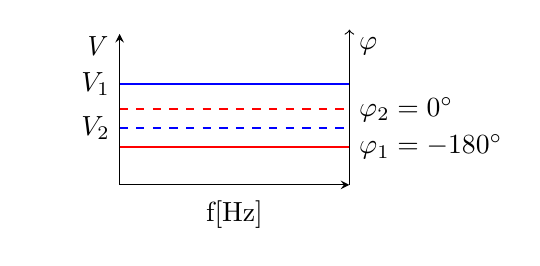
\begin{tikzpicture}[scale=1, transform shape]
    \begin{axis}[
        width=4.5cm, % Breite des Graphen
        height=3.5cm, % Höhe des Graphen
        xmin=0, xmax=10,
        ymin=0, ymax=120,
        axis lines=left,
        axis on top=true,
        domain=0:10,
        xtick=\empty,
        ytick=\empty,
        ylabel style={rotate=270, anchor=east, yshift=0.8cm},
         ylabel={\it V},
        xlabel={f[Hz]},
        clip mode=individual % Verhindert das Abschneiden von Elementen
        ]
        \path[draw=none] (axis cs:-4, 0) rectangle (axis cs:16.6,120);

        \addplot+[mark=none, thick, blue] coordinates {(0,80) (10,80)};
        \addplot+[mark=none, thick, blue, dashed] coordinates {(0,45) (10,45)};
        % Adding the left-side label
        \node[anchor=east] at (axis cs:0,80) {$V_1$};
        \node[anchor=east] at (axis cs:0,45) {$V_2$};
    \end{axis}
    \begin{axis}[
        width=4.5cm, % Breite des Graphen
        height=3.5cm, % Höhe des Graphen
        xmin=0, xmax=10,
        ymin=-180, ymax=180,
        axis y line*=right,
        axis x line=none,
        ytick=\empty,
        ylabel={$\varphi$},
        ylabel style={rotate=270, anchor=west, yshift=0.8cm},
        clip mode=individual, % Verhindert das Abschneiden von Elementen
        after end axis/.code={
            \draw[->] (axis cs:10,180) -- (axis cs:10,190);
        }
        ]
        \addplot+[mark=none, thick, red, dashed] coordinates {(0,0) (10,0)};
        \addplot+[mark=none, thick, red] coordinates {(0,-90) (10,-90)};
        \node[anchor=west] at (axis cs:10,0) {$\varphi_2 = 0^\circ$};
        \node[anchor=west] at (axis cs:10,-90) {$\varphi_1 = -180^\circ$};
    \end{axis}
    \end{tikzpicture}
\[
V_1: U_{\textnormal{E+}} > U_{\textnormal{E-}} \Rightarrow U_{\textnormal{A}} \approx +U_{\textnormal{B}}
\]
\[
V_2: U_{\textnormal{E+}} < U_{\textnormal{E-}} \Rightarrow U_{\textnormal{A}} \approx -U_{\textnormal{B}}
\]
\end{center}
    &\textbf{Komparator}\newline
    Einsatz in Zweipunktreglern und Analog-Digital-Wandlern \\
    \hline
    \end{tabular}
    \end{table}
    }
\end{frame}

\begin{frame}
    \b{
    \frametitle{Komparator neu}
    \begin{columns}
        \column{0.48\textwidth}
        \centering
        \begin{figure}
    \centering

    \begin{subfigure}{\linewidth}
        \centering
        \resizebox{0.6\linewidth}{!}{\begin{circuitikz}[scale=0.7, transform shape]
    \ctikzset{
          resistors/scale=0.8,              
          tripoles/en amp/height=1.4, % Höhe des OPV             
          tripoles/en amp/width=1.4,   % Breite des OPV
         tripoles/en amp/input height=0.45
     }
     \draw
     (0,0) node[en amp] (opamp) {}
     (opamp.-)  to[short, o-] ++(0,0) node[left] {$U_{E-}$}
      (opamp.+) to[short, o-] ++(0,0) node[left] {$U_{E+}$}
     (opamp.out) to[short, -o] ++(0,0) node[right] {$U_{A}$};
 \end{circuitikz}}
        \caption{Schaltung eines Komparators}
    \end{subfigure}

    \vspace{0.5cm} 

    \begin{subfigure}{\linewidth}
        \centering
        \resizebox{0.6\linewidth}{!}{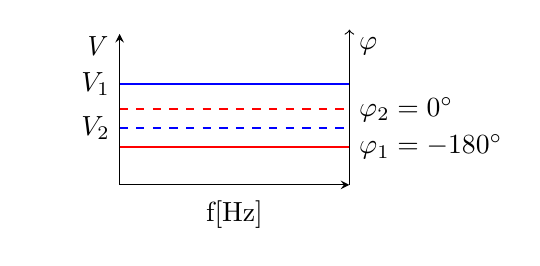
\begin{tikzpicture}[scale=1, transform shape]
    \begin{axis}[
        width=4.5cm, % Breite des Graphen
        height=3.5cm, % Höhe des Graphen
        xmin=0, xmax=10,
        ymin=0, ymax=120,
        axis lines=left,
        axis on top=true,
        domain=0:10,
        xtick=\empty,
        ytick=\empty,
        ylabel style={rotate=270, anchor=east, yshift=0.8cm},
         ylabel={\it V},
        xlabel={f[Hz]},
        clip mode=individual % Verhindert das Abschneiden von Elementen
        ]
        \path[draw=none] (axis cs:-4, 0) rectangle (axis cs:16.6,120);

        \addplot+[mark=none, thick, blue] coordinates {(0,80) (10,80)};
        \addplot+[mark=none, thick, blue, dashed] coordinates {(0,45) (10,45)};
        % Adding the left-side label
        \node[anchor=east] at (axis cs:0,80) {$V_1$};
        \node[anchor=east] at (axis cs:0,45) {$V_2$};
    \end{axis}
    \begin{axis}[
        width=4.5cm, % Breite des Graphen
        height=3.5cm, % Höhe des Graphen
        xmin=0, xmax=10,
        ymin=-180, ymax=180,
        axis y line*=right,
        axis x line=none,
        ytick=\empty,
        ylabel={$\varphi$},
        ylabel style={rotate=270, anchor=west, yshift=0.8cm},
        clip mode=individual, % Verhindert das Abschneiden von Elementen
        after end axis/.code={
            \draw[->] (axis cs:10,180) -- (axis cs:10,190);
        }
        ]
        \addplot+[mark=none, thick, red, dashed] coordinates {(0,0) (10,0)};
        \addplot+[mark=none, thick, red] coordinates {(0,-90) (10,-90)};
        \node[anchor=west] at (axis cs:10,0) {$\varphi_2 = 0^\circ$};
        \node[anchor=west] at (axis cs:10,-90) {$\varphi_1 = -180^\circ$};
    \end{axis}
    \end{tikzpicture}}
        \caption{Frequenzgang eines Komparators}
    \end{subfigure}

\end{figure}

        \column{0.48\textwidth}
        \begin{itemize}
            \item Gleichung:
          \[
V_1: U_{\textnormal{E+}} > U_{\textnormal{E-}} \Rightarrow U_{\textnormal{A}} \approx +U_{\textnormal{B}}
\]
\[
V_2: U_{\textnormal{E+}} < U_{\textnormal{E-}} \Rightarrow U_{\textnormal{A}} \approx -U_{\textnormal{B}}
\]
    \item Einsatz in Zweipunktreglern und Analog-Digital-Wandlern
        \end{itemize}
    \end{columns}
    }
\end{frame}

%Folie Summierer

\begin{frame}
    \b{
    \frametitle{Summierer}
    \centering
    \begin{table}[ht]
    \label{tab:Summierer}
    \begin{tabular}{|m{0.24\textwidth}|m{0.405\textwidth}|m{0.25\textwidth}|}
    \hline
    Schaltung & Frequenzgang und Gleichung & Erläuterung und Eigenschaften\\ % Neue Zeile mit Text
    \hline
    \vspace{0.5cm}
    \centering
    \begin{circuitikz}[scale=0.7, transform shape]
    \ctikzset{
        resistors/scale=0.8,              
        tripoles/en amp/height=1.4, % Höhe des OPV             
        tripoles/en amp/width=1.4,   % Breite des OPV
        tripoles/en amp/input height=0.45
    }
    \draw
    (0,0) node[en amp] (opamp) {}
    % R2 mit korrigiertem Strompfeil
    (opamp.-) -- ++(-0.4,0) node[circ] {} to[R, l_=$R_2$] ++(-1.5,0) node[ocirc] (R2left) {}
    % R1 mit korrigiertem Strompfeil
    (opamp.-) -- ++(-0.4,0) --++(0,1) to[R, l_=$R_1$] ++(-1.5,0) node[ocirc] (R1left) {}
    % Erdung
    (opamp.+) -- ++(0,0) node[ground] {}
    % Ausgang
    (opamp.out) to[short, *-o] ++(0,0) node[right] {$U_{A}$}
    % R3 mit Strompfeil
    (opamp.out) -- ++(0,1.5) to[R, l_=$R_3$] ++(-2,0) -- ++(0,-1.05) node[circ] {}
    % Spannungen U_E1 und U_E2 an den Knoten links von R1 und R2
    (R1left) node[left] {$U_{E1}$}
    (R2left) node[left] {$U_{E2}$};
\end{circuitikz}

    &
    \begin{center}
    \input{Tikz/src/FrequenzgangSummierer.tex}
\end{center}
\vspace{1ex}
\[
\begin{aligned}
    U_{\textnormal{A}} = \underbrace{\frac{R_3} {R_1}}_{V_1} \cdot U_{\textnormal{E1}} + \underbrace{\frac{R_3} {R_2}}_{V_2} \cdot U_{\textnormal{E2}}
\end{aligned}
\]
    & 
    Der Summierer basiert auf dem invertierenden Verstärker und findet Verwendung in Analogrechnern und beim Mischen von Spannungssignalen \\
    \hline
    \end{tabular}
    \end{table}
    }
\end{frame}

\begin{frame}
    \b{
    \frametitle{Summierer neu}
    \begin{columns}
        \column{0.48\textwidth}
        \centering
        \begin{figure}
    \centering

    \begin{subfigure}{\linewidth}
        \centering
        \resizebox{0.6\linewidth}{!}{\begin{circuitikz}[scale=0.7, transform shape]
    \ctikzset{
        resistors/scale=0.8,              
        tripoles/en amp/height=1.4, % Höhe des OPV             
        tripoles/en amp/width=1.4,   % Breite des OPV
        tripoles/en amp/input height=0.45
    }
    \draw
    (0,0) node[en amp] (opamp) {}
    % R2 mit korrigiertem Strompfeil
    (opamp.-) -- ++(-0.4,0) node[circ] {} to[R, l_=$R_2$] ++(-1.5,0) node[ocirc] (R2left) {}
    % R1 mit korrigiertem Strompfeil
    (opamp.-) -- ++(-0.4,0) --++(0,1) to[R, l_=$R_1$] ++(-1.5,0) node[ocirc] (R1left) {}
    % Erdung
    (opamp.+) -- ++(0,0) node[ground] {}
    % Ausgang
    (opamp.out) to[short, *-o] ++(0,0) node[right] {$U_{A}$}
    % R3 mit Strompfeil
    (opamp.out) -- ++(0,1.5) to[R, l_=$R_3$] ++(-2,0) -- ++(0,-1.05) node[circ] {}
    % Spannungen U_E1 und U_E2 an den Knoten links von R1 und R2
    (R1left) node[left] {$U_{E1}$}
    (R2left) node[left] {$U_{E2}$};
\end{circuitikz}}
        \caption{Schaltung eines Summierers}
    \end{subfigure}

    \vspace{0.5cm} 

    \begin{subfigure}{\linewidth}
        \centering
        \resizebox{0.6\linewidth}{!}{\input{Tikz/src/FrequenzgangSummierer.tex}}
        \caption{Frequenzgang eines Summierers}
    \end{subfigure}

\end{figure}

        \column{0.48\textwidth}
        \begin{itemize}
            \item Gleichung:
          \[
U_{\textnormal{A}} = \underbrace{\frac{R_3} {R_1}}_{V_1} \cdot U_{\textnormal{E1}} + \underbrace{\frac{R_3} {R_2}}_{V_2} \cdot U_{\textnormal{E2}}
\]
    \item Der Summierer basiert auf dem invertierenden Verstärker und findet Verwendung in Analogrechnern und beim Mischen von Spannungssignalen
        \end{itemize}
    \end{columns}
    }
\end{frame}

%Folie Subtrahierer

\begin{frame}
    \b{
    \frametitle{Subtrahierer}
    \centering
    \begin{table}[ht]
    \label{tab:Subtrahierer}
    \begin{tabular}{|m{0.24\textwidth}|m{0.405\textwidth}|m{0.25\textwidth}|}
    \hline
    Schaltung & Frequenzgang und Gleichung & Erläuterung und Eigenschaften\\ % Neue Zeile mit Text
    \hline
    \vspace{0.5cm}
    \centering
    \begin{circuitikz}[scale=0.7, transform shape]
    \ctikzset{
          resistors/scale=0.8,              
          tripoles/en amp/height=1.4, % Höhe des OPV             
          tripoles/en amp/width=1.4,   % Breite des OPV
         tripoles/en amp/input height=0.45
     }
     \draw
     (0,0) node[en amp] (opamp) {}
     (opamp.-) to[R, l_=$R_1$, o-] ++(-1.2,0) to[short, o-] ++(0,0) node[left] {$U_{E1}$}
     (opamp.+) node[circ] {} to[R,  l_=$R_4$] ++(0,-1.5) node[ground] {}
     (opamp.-) node[circ] {} -- ++(0,1) to[R, l=$R_2$] ++(1.9,0) -| (opamp.out)
     (opamp.out) to[short, *-o] ++(0.2,0) node[right] {$U_{A}$}
     (opamp.+) to[R, l_=$R_3$, *-] ++(-1.2,0) to[short, o-] ++(0,0) node[left] {$U_{E2}$};
 \end{circuitikz}
      &
      \begin{center}
      \input{Tikz/src/FrequenzgangSubtrahierer.tex}
 \end{center}
 \vspace{1ex}
 \[
 \begin{aligned}
    {U_A} = {U_{{\textnormal{E2}}}} \cdot \underbrace{ \frac{R_1 + R_2}{R_1} \cdot \frac{R_4}{R_3 + R_4}}_{V_2} - U_{\textnormal{E1}} \cdot \underbrace{\frac{R_2}{R_1}}_{V_1}
\end{aligned}
 \]
     &
     Wenn alle Widerstände gleich groß sind, wird die Differenz der Signale $U_{E1}$ und $U_{E2}$ gebildet, weswegen diese Schaltung als Differenzverstärker bezeichnet wird \\
    \hline
    \end{tabular}
    \end{table}
    }
\end{frame}

\begin{frame}
    \b{
    \frametitle{Subtrahierer neu}
    \begin{columns}
        \column{0.48\textwidth}
        \centering
        \begin{figure}
    \centering

    \begin{subfigure}{\linewidth}
        \centering
        \resizebox{0.6\linewidth}{!}{\begin{circuitikz}[scale=0.7, transform shape]
    \ctikzset{
          resistors/scale=0.8,              
          tripoles/en amp/height=1.4, % Höhe des OPV             
          tripoles/en amp/width=1.4,   % Breite des OPV
         tripoles/en amp/input height=0.45
     }
     \draw
     (0,0) node[en amp] (opamp) {}
     (opamp.-) to[R, l_=$R_1$, o-] ++(-1.2,0) to[short, o-] ++(0,0) node[left] {$U_{E1}$}
     (opamp.+) node[circ] {} to[R,  l_=$R_4$] ++(0,-1.5) node[ground] {}
     (opamp.-) node[circ] {} -- ++(0,1) to[R, l=$R_2$] ++(1.9,0) -| (opamp.out)
     (opamp.out) to[short, *-o] ++(0.2,0) node[right] {$U_{A}$}
     (opamp.+) to[R, l_=$R_3$, *-] ++(-1.2,0) to[short, o-] ++(0,0) node[left] {$U_{E2}$};
 \end{circuitikz}}
        \caption{Schaltung eines Subtrahierers}
    \end{subfigure}

    \vspace{0.5cm} 

    \begin{subfigure}{\linewidth}
        \centering
        \resizebox{0.6\linewidth}{!}{\input{Tikz/src/FrequenzgangSubtrahierer.tex}}
        \caption{Frequenzgang eines Subtrahierers}
    \end{subfigure}

\end{figure}

        \column{0.48\textwidth}
        \raggedleft
        \begin{itemize}
            \item Gleichung:
          \[
 {U_A} = {U_{{\textnormal{E2}}}} \cdot \underbrace{ \frac{R_1 + R_2}{R_1} \cdot \frac{R_4}{R_3 + R_4}}_{V_2} - U_{\textnormal{E1}} \cdot \underbrace{\frac{R_2}{R_1}}_{V_1}
          \]
    \item Wenn alle Widerstände gleich groß sind, wird die Differenz der Signale $U_{E1}$ und $U_{E2}$ gebildet, weswegen diese Schaltung als Differenzverstärker bezeichnet wird
        \end{itemize}
    \end{columns}
    }
\end{frame}


%Folie Integrierer

\begin{frame}
    \b{
    \frametitle{Integrierer}
    \centering
    \begin{table}[ht]
    \label{tab:Integrierer}
    \begin{tabular}{|m{0.24\textwidth}|m{0.405\textwidth}|m{0.25\textwidth}|}
    \hline
    Schaltung & Frequenzgang und Gleichung & Erläuterung und Eigenschaften\\ % Neue Zeile mit Text
    \hline
    \vspace{0.5cm}
    \centering
    \begin{circuitikz}[scale=0.7, transform shape]
    \ctikzset{
          resistors/scale=0.8,              
          tripoles/en amp/height=1.4, % Höhe des OPV             
          tripoles/en amp/width=1.4,   % Breite des OPV
         capacitors/scale=0.5,
         tripoles/en amp/input height=0.45
     }
     \vspace{1ex}
     \draw (2,0) node[en amp] (opamp) {}
     (opamp.+) --++ (-0.5,0) node[ground] {} 
     (opamp.out) --++ (0.2,0) node[ocirc, label=right:$U_A$] {}
     (opamp.-) -- ++(0, 0) to[R, l_=$R_1$] ++(-1.2, 0) node[ocirc, label=left:$U_E$] {}
     
     (opamp.out) node[circ] {} -- ++(0,1.5) to[C, l_=$C_1$, *-] ++(-1.9,0) node[circ]{}
     (opamp.out) node[circ] {} -- ++(0,2.8) to[R, l_=$R_2$] ++(-1.9,0) -- ++(0, -2.35) node[circ] {};
     \end{circuitikz}
     & 
     \begin{center}
    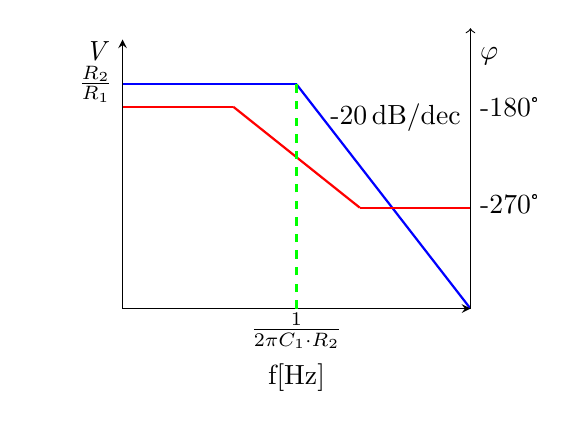
\begin{tikzpicture}[scale=1, transform shape]
    \begin{axis}[
       width=6cm, % Breite des Graphen
       height=5cm, % Höhe des Graphen
        xmin=0, xmax=11,
        ymin=0, ymax=1.2,
        axis lines=center,
        axis on top=true,
        domain=0:10,
        xtick=\empty,
        ytick=\empty,
        ylabel style={xshift=-0.6cm, yshift=0.1cm },
       ylabel={\it V},
       xlabel style={yshift=-0.4cm },
        xlabel={f[Hz]},
        clip mode=individual, % Verhindert das Abschneiden von Elementen
        xlabel style={at={(axis description cs:0.5,-0.05)},anchor=north}
        ]

        \path[draw=none] (axis cs:-3, 0) rectangle (axis cs:13,1);



        \addplot+[mark=none, thick, blue] coordinates {(0,1) (5.5,1)};
        \addplot+[mark=none, thick, blue] coordinates {(5.5,1) (11,0)};
        \node[anchor=east] at (axis cs:0,1) {$\frac{R_2}{R_1}$};
       \node[anchor=east] at (axis cs:11,0.85) {-20\,\text{dB/dec}};
    \end{axis}
    
    \begin{axis}[
       width=6cm, % Breite des Graphen
       height=5cm, % Höhe des Graphen
       xmin=0, xmax=11,
       ymin=0, ymax=240, 
       axis y line*=right,
       axis x line=none,
       ylabel={$\varphi$},
       ylabel style={rotate=270, anchor=west, yshift=1.5cm},
       xtick=\empty,
       ytick=\empty,
       clip mode=individual, % Verhindert das Abschneiden von Elementen
       after end axis/.code={
           \draw[->] (axis cs:11,240) -- (axis cs:11,250);
       }
        ]
        \addplot+[mark=none, thick, red] coordinates {(0,180) (3.5,180)};
        \addplot+[mark=none, thick, red] coordinates {(3.5,180) (7.5,90)};
        \addplot+[mark=none, thick, red] coordinates {(7.5,90) (11,90)};
        \addplot+[mark=none,dashed, thick, green] coordinates {(5.5,0) (5.5,200)};
        \node[] at (axis cs:5.5,-20) {$\frac{1}{2 \pi C_1 \cdot R_2}$};
        \node[anchor=west] at (axis cs:11,180) {-180°};
        \node[anchor=west] at (axis cs:11,93) {-270°};
    \end{axis}
    \end{tikzpicture}
     \[
     U_A(t) = - \frac{R_2}{R_1} U_{\textnormal{E}}(t) - \int_0^t \frac{U_{\textnormal{E}}(t)}{R_1 C_1} \, dt
     \]
     \end{center} 
     &
    \begin{itemize}
        \item Nimmt eine Integration des Eingangssignals vor
        \item Wird als aktives Tiefpassfilter verwendet
    \end{itemize} \\
    \hline
    \end{tabular}
    \end{table}
    }
\end{frame}

\begin{frame}
    \b{
    \frametitle{Integrierer neu}
    \begin{columns}
        \column{0.48\textwidth}
        \centering
        \begin{figure}
    \centering

    \begin{subfigure}{\linewidth}
        \centering
        \resizebox{0.6\linewidth}{!}{\begin{circuitikz}[scale=0.7, transform shape]
    \ctikzset{
          resistors/scale=0.8,              
          tripoles/en amp/height=1.4, % Höhe des OPV             
          tripoles/en amp/width=1.4,   % Breite des OPV
         capacitors/scale=0.5,
         tripoles/en amp/input height=0.45
     }
     \vspace{1ex}
     \draw (2,0) node[en amp] (opamp) {}
     (opamp.+) --++ (-0.5,0) node[ground] {} 
     (opamp.out) --++ (0.2,0) node[ocirc, label=right:$U_A$] {}
     (opamp.-) -- ++(0, 0) to[R, l_=$R_1$] ++(-1.2, 0) node[ocirc, label=left:$U_E$] {}
     
     (opamp.out) node[circ] {} -- ++(0,1.5) to[C, l_=$C_1$, *-] ++(-1.9,0) node[circ]{}
     (opamp.out) node[circ] {} -- ++(0,2.8) to[R, l_=$R_2$] ++(-1.9,0) -- ++(0, -2.35) node[circ] {};
     \end{circuitikz}}
        \caption{Schaltung eines Integrierers}
    \end{subfigure}

    \vspace{0.5cm} 

    \begin{subfigure}{\linewidth}
        \centering
        \resizebox{0.6\linewidth}{!}{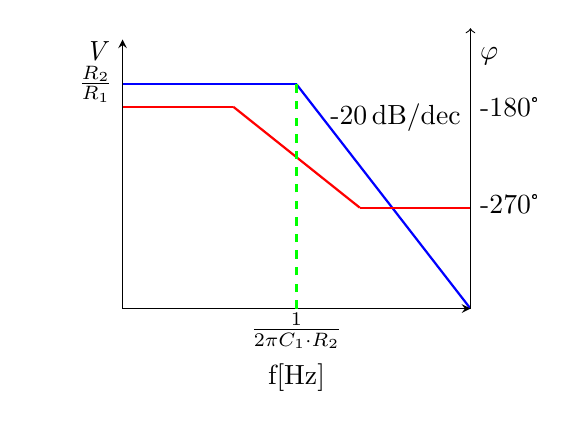
\begin{tikzpicture}[scale=1, transform shape]
    \begin{axis}[
       width=6cm, % Breite des Graphen
       height=5cm, % Höhe des Graphen
        xmin=0, xmax=11,
        ymin=0, ymax=1.2,
        axis lines=center,
        axis on top=true,
        domain=0:10,
        xtick=\empty,
        ytick=\empty,
        ylabel style={xshift=-0.6cm, yshift=0.1cm },
       ylabel={\it V},
       xlabel style={yshift=-0.4cm },
        xlabel={f[Hz]},
        clip mode=individual, % Verhindert das Abschneiden von Elementen
        xlabel style={at={(axis description cs:0.5,-0.05)},anchor=north}
        ]

        \path[draw=none] (axis cs:-3, 0) rectangle (axis cs:13,1);



        \addplot+[mark=none, thick, blue] coordinates {(0,1) (5.5,1)};
        \addplot+[mark=none, thick, blue] coordinates {(5.5,1) (11,0)};
        \node[anchor=east] at (axis cs:0,1) {$\frac{R_2}{R_1}$};
       \node[anchor=east] at (axis cs:11,0.85) {-20\,\text{dB/dec}};
    \end{axis}
    
    \begin{axis}[
       width=6cm, % Breite des Graphen
       height=5cm, % Höhe des Graphen
       xmin=0, xmax=11,
       ymin=0, ymax=240, 
       axis y line*=right,
       axis x line=none,
       ylabel={$\varphi$},
       ylabel style={rotate=270, anchor=west, yshift=1.5cm},
       xtick=\empty,
       ytick=\empty,
       clip mode=individual, % Verhindert das Abschneiden von Elementen
       after end axis/.code={
           \draw[->] (axis cs:11,240) -- (axis cs:11,250);
       }
        ]
        \addplot+[mark=none, thick, red] coordinates {(0,180) (3.5,180)};
        \addplot+[mark=none, thick, red] coordinates {(3.5,180) (7.5,90)};
        \addplot+[mark=none, thick, red] coordinates {(7.5,90) (11,90)};
        \addplot+[mark=none,dashed, thick, green] coordinates {(5.5,0) (5.5,200)};
        \node[] at (axis cs:5.5,-20) {$\frac{1}{2 \pi C_1 \cdot R_2}$};
        \node[anchor=west] at (axis cs:11,180) {-180°};
        \node[anchor=west] at (axis cs:11,93) {-270°};
    \end{axis}
    \end{tikzpicture}}
        \caption{Frequenzgang eines Integrierers}
    \end{subfigure}

\end{figure}

        \column{0.48\textwidth}
        \raggedleft
        \begin{itemize}
            \item Gleichung:
           \[
     U_A(t) = - \frac{R_2}{R_1} U_{\textnormal{E}}(t) - \int_0^t \frac{U_{\textnormal{E}}(t)}{R_1 C_1} \, dt
     \]
        \item Nimmt eine Integration des Eingangssignals vor
        \item Wird als aktives Tiefpassfilter verwendet     
    \end{itemize}
    \end{columns}
    }
\end{frame}

%Folie Differenzierer

\begin{frame}
    \b{
    \frametitle{Differenzierer}
    \centering
    \begin{table}[ht]
    \label{tab:Differenzierer}
    \begin{tabular}{|m{0.24\textwidth}|m{0.405\textwidth}|m{0.25\textwidth}|}
    \hline
    Schaltung & Frequenzgang und Gleichung & Erläuterung und Eigenschaften\\ % Neue Zeile mit Text
    \hline
    \vspace{0.5cm}
    \centering
    \input{Tikz/src/Differenzierer.tex}
    &
    \begin{center}
    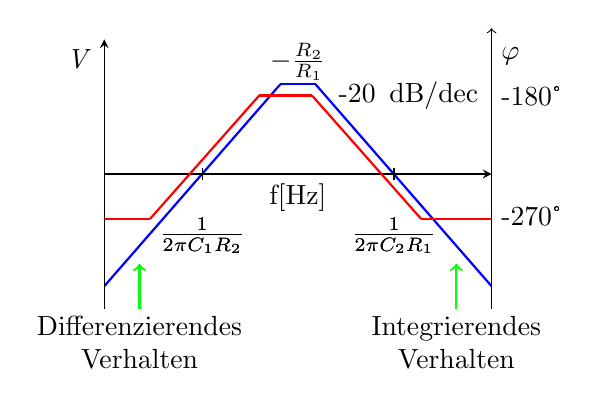
\begin{tikzpicture}[scale=1, transform shape]
    \begin{axis}[
        width=6.5cm, % Breite des Graphen
        height=5cm, % Höhe des Graphen
        xmin=0, xmax=11,
        ymin=-1.2, ymax=1.2,
        axis lines=center,
        axis on top=true,
        domain=0:10,
        clip mode=individual, % Verhindert das Abschneiden von Elementen
        xtick=\empty,
        ytick=\empty,
        ylabel style={xshift=-0.6cm},
        ylabel={\it V},
        xlabel={f[Hz]},
        xlabel style={at={(axis description cs:0.5,0.5)},anchor=north}
        ]
        \path[draw=none] (axis cs:-2, 0) rectangle (axis cs:13,1); \path[draw=none] (axis cs:-2, 0) rectangle (axis cs:13,1);


        \addplot+[mark=none, thick, blue] coordinates {(0,-1) (5,0.8)};
        \addplot+[mark=none, thick, blue] coordinates {(5,0.8) (6,0.8)};
        \addplot+[mark=none, thick, blue] coordinates {(6,0.8) (11,-1)};
        \node[anchor=north] at (axis cs:5.5,1.25) {$-\frac{R_2}{R_1}$};
        \addplot+[only marks, mark=|, black] coordinates {(2.78,0)} node[anchor=south] at (axis cs:2.78,-0.8) {$\frac{1}{2 \pi C_1 R_2}$};
        \addplot+[only marks, mark=|, black] coordinates {(8.23,0)} node[anchor=south] at (axis cs:8.23,-0.8) {$\frac{1}{2\pi C_2 R_1}$};
        \node[anchor=east] at (axis cs:10.9,0.7) {-20\, \text{dB/dec}};
        \addplot+[only marks, mark=|, black] coordinates {(2.78,0)} node[anchor=south] at (axis cs:2.78,-0.8) {$\frac{1}{2 \pi C_1 R_2}$};
        \addplot+[only marks, mark=|, black] coordinates {(8.23,0)} node[anchor=south] at (axis cs:8.23,-0.8) {$\frac{1}{2\pi C_2 R_1}$};
        \draw[->, thick, green] (axis cs:1,-1.2) -- (axis cs:1,-0.8);
        \node[align=center, black] at (axis cs:1,-1.5) {Differenzierendes\\ Verhalten};
        
        \draw[->, thick, green] (axis cs:10,-1.2) -- (axis cs:10,-0.8);
        \node[align=center, black] at (axis cs:10,-1.5) {Integrierendes\\ Verhalten};
        
    \end{axis}
    
    \begin{axis}[
        width=6.5cm, % Breite des Graphen
        height=5cm, % Höhe des Graphen
        xmin=0, xmax=11,
        ymin=0, ymax=240, 
        axis y line*=right,
        axis x line=none,
        ylabel={$\varphi$},
        ylabel style={rotate=270, anchor=west, yshift=1.5cm},
        xtick=\empty,
        ytick=\empty,
        clip mode=individual, % Verhindert das Abschneiden von Elementen
        after end axis/.code={
            \draw[->] (axis cs:11,240) -- (axis cs:11,250);
        }
        ]
        \addplot+[mark=none, thick, red] coordinates {(0,80) (1.3,80)};
        \addplot+[mark=none, thick, red] coordinates {(1.3,80) (4.4,190)};
        \addplot+[mark=none, thick, red] coordinates {(4.4,190) (5.9,190)};
        \addplot+[mark=none, thick, red] coordinates {(5.9,190) (9,80)};
        \addplot+[mark=none, thick, red] coordinates {(9,80) (11,80)};
        \node[anchor=west] at (axis cs:11,82.5) {-270°};
        \node[anchor=west] at (axis cs:11,190) {-180°};
       
    \end{axis}

    
    \end{tikzpicture}
    \begin{multline*}
        U_A = - \frac{R_2}{R_1} U_{\textnormal{E}}(t) \\
        - \int_0^t \frac{1}{R_1 C_1} U_{\textnormal{E}}(t) \, dt 
        - R_2 C_2\frac{dU_{\textnormal{E}}(t)}{dt}
    \end{multline*}
    \end{center} 
    & 
    \textbf{Differenzierer}\newline
    \begin{itemize}
        \item Nimmt eine Integration des Eingangssignals vor
        \item Wird als aktives Hochpassfilter verwendet (zeigt in der Realität meist Bandpassverhalten, wie hier dargestellt)
    \end{itemize} \\
    \hline
    \end{tabular}
    \end{table}
    }
\end{frame}

\begin{frame}
    \b{
    \frametitle{Differenzierer neu}
    \begin{columns}
        \column{0.48\textwidth}
        \centering
        \begin{figure}
    \centering

    \begin{subfigure}{\linewidth}
        \centering
        \resizebox{0.6\linewidth}{!}{\input{Tikz/src/Differenzierer.tex}}
        \caption{Schaltung eines Differenzierers}
    \end{subfigure}

    \vspace{0.5cm} 

    \begin{subfigure}{\linewidth}
        \centering
        \resizebox{0.6\linewidth}{!}{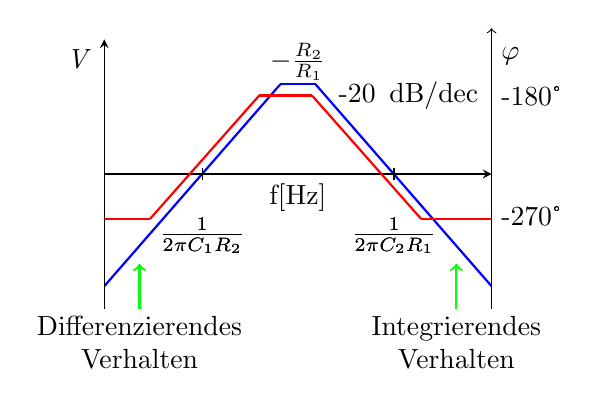
\begin{tikzpicture}[scale=1, transform shape]
    \begin{axis}[
        width=6.5cm, % Breite des Graphen
        height=5cm, % Höhe des Graphen
        xmin=0, xmax=11,
        ymin=-1.2, ymax=1.2,
        axis lines=center,
        axis on top=true,
        domain=0:10,
        clip mode=individual, % Verhindert das Abschneiden von Elementen
        xtick=\empty,
        ytick=\empty,
        ylabel style={xshift=-0.6cm},
        ylabel={\it V},
        xlabel={f[Hz]},
        xlabel style={at={(axis description cs:0.5,0.5)},anchor=north}
        ]
        \path[draw=none] (axis cs:-2, 0) rectangle (axis cs:13,1); \path[draw=none] (axis cs:-2, 0) rectangle (axis cs:13,1);


        \addplot+[mark=none, thick, blue] coordinates {(0,-1) (5,0.8)};
        \addplot+[mark=none, thick, blue] coordinates {(5,0.8) (6,0.8)};
        \addplot+[mark=none, thick, blue] coordinates {(6,0.8) (11,-1)};
        \node[anchor=north] at (axis cs:5.5,1.25) {$-\frac{R_2}{R_1}$};
        \addplot+[only marks, mark=|, black] coordinates {(2.78,0)} node[anchor=south] at (axis cs:2.78,-0.8) {$\frac{1}{2 \pi C_1 R_2}$};
        \addplot+[only marks, mark=|, black] coordinates {(8.23,0)} node[anchor=south] at (axis cs:8.23,-0.8) {$\frac{1}{2\pi C_2 R_1}$};
        \node[anchor=east] at (axis cs:10.9,0.7) {-20\, \text{dB/dec}};
        \addplot+[only marks, mark=|, black] coordinates {(2.78,0)} node[anchor=south] at (axis cs:2.78,-0.8) {$\frac{1}{2 \pi C_1 R_2}$};
        \addplot+[only marks, mark=|, black] coordinates {(8.23,0)} node[anchor=south] at (axis cs:8.23,-0.8) {$\frac{1}{2\pi C_2 R_1}$};
        \draw[->, thick, green] (axis cs:1,-1.2) -- (axis cs:1,-0.8);
        \node[align=center, black] at (axis cs:1,-1.5) {Differenzierendes\\ Verhalten};
        
        \draw[->, thick, green] (axis cs:10,-1.2) -- (axis cs:10,-0.8);
        \node[align=center, black] at (axis cs:10,-1.5) {Integrierendes\\ Verhalten};
        
    \end{axis}
    
    \begin{axis}[
        width=6.5cm, % Breite des Graphen
        height=5cm, % Höhe des Graphen
        xmin=0, xmax=11,
        ymin=0, ymax=240, 
        axis y line*=right,
        axis x line=none,
        ylabel={$\varphi$},
        ylabel style={rotate=270, anchor=west, yshift=1.5cm},
        xtick=\empty,
        ytick=\empty,
        clip mode=individual, % Verhindert das Abschneiden von Elementen
        after end axis/.code={
            \draw[->] (axis cs:11,240) -- (axis cs:11,250);
        }
        ]
        \addplot+[mark=none, thick, red] coordinates {(0,80) (1.3,80)};
        \addplot+[mark=none, thick, red] coordinates {(1.3,80) (4.4,190)};
        \addplot+[mark=none, thick, red] coordinates {(4.4,190) (5.9,190)};
        \addplot+[mark=none, thick, red] coordinates {(5.9,190) (9,80)};
        \addplot+[mark=none, thick, red] coordinates {(9,80) (11,80)};
        \node[anchor=west] at (axis cs:11,82.5) {-270°};
        \node[anchor=west] at (axis cs:11,190) {-180°};
       
    \end{axis}

    
    \end{tikzpicture}}
        \caption{Frequenzgang eines Differenzierers}
    \end{subfigure}

\end{figure}

        \column{0.48\textwidth}
        \raggedleft
        \begin{itemize}
            \item Gleichung:
          \[
U_{\textnormal{A}}(t) = 
- \frac{R_2}{R_1} \, U_{\textnormal{E}}(t)
- \int_0^t \frac{1}{R_1 C_1} \, U_{\textnormal{E}}(\tau) \, d\tau
- R_2 C_2 \, \frac{dU_{\textnormal{E}}}{dt}(t)
\]

        \item Nimmt eine Integration des Eingangssignals vor
        \item Wird als aktives Hochpassfilter verwendet (zeigt in der Realität meist Bandpassverhalten, wie hier dargestellt)  
    \end{itemize}
    \end{columns}
    }
\end{frame}

%Folie Logarithmierer

\begin{frame}
    \b{
    \frametitle{Logarithmierer}
    \centering
    \begin{table}[ht]
    \label{tab:Logarithmierer}
    \begin{tabular}{|m{0.24\textwidth}|m{0.405\textwidth}|m{0.25\textwidth}|}
    \hline
    Schaltung & Frequenzgang und Gleichung & Erläuterung und Eigenschaften\\ % Neue Zeile mit Text
    \hline
    \vspace{0.5cm}
    \centering
    \begin{circuitikz}[scale=0.7, transform shape]
    \ctikzset{
          resistors/scale=0.8,              
          tripoles/en amp/height=1.4, % Höhe des OPV             
          tripoles/en amp/width=1.4,   % Breite des OPV
         diodes/scale=0.8,
         tripoles/en amp/input height=0.45
     }
     \draw
     (0,0) node[en amp] (opamp) {}
     (opamp.-) to[R, l_=$R_1$, *-] ++(-1.2,0) to[short, o-] ++(0,0) node[left] {$U_E$}
     (opamp.+) -- ++(0,0) node[ground] {}
     (opamp.-) |- ++(0,1.5) to[D, l^=$D_1$] ++(2,0) -| (opamp.out)
     (opamp.out) to[short, *-o] ++(0.2,0) node[right] {$U_{A}$};
 \end{circuitikz}
    &
    \begin{center}
    \[
    U_{\textnormal{A}} =-U_{\textnormal{T}}\cdot \ln{\left(\frac{U_{\textnormal{E}}}{R_1\cdot I_S}\right)}
    \]
        \[
            U_{\textnormal{T}} = \frac{k_{\textnormal{B}} \cdot T}{e}
            \]
            
            \(e = \text{Elementarladung}\)
            
            \(k_{\textnormal{B}} = \text{Boltzmannkonstante}\)
            
            \(I_{\textnormal{s}} = \text{Sperrstrom der Diode}\)
    \end{center} 
    & 
    Bildet den natürlichen Logarithmus des Eingangssignals \\
    \hline
    \end{tabular}
    \end{table}
    }
\end{frame}

\begin{frame}
    \b{
    \frametitle{Logarithmierer neu}
    \begin{columns}
        \column{0.48\textwidth}
        \centering
        \begin{figure}
    \centering
        \begin{circuitikz}[scale=0.7, transform shape]
    \ctikzset{
          resistors/scale=0.8,              
          tripoles/en amp/height=1.4, % Höhe des OPV             
          tripoles/en amp/width=1.4,   % Breite des OPV
         diodes/scale=0.8,
         tripoles/en amp/input height=0.45
     }
     \draw
     (0,0) node[en amp] (opamp) {}
     (opamp.-) to[R, l_=$R_1$, *-] ++(-1.2,0) to[short, o-] ++(0,0) node[left] {$U_E$}
     (opamp.+) -- ++(0,0) node[ground] {}
     (opamp.-) |- ++(0,1.5) to[D, l^=$D_1$] ++(2,0) -| (opamp.out)
     (opamp.out) to[short, *-o] ++(0.2,0) node[right] {$U_{A}$};
 \end{circuitikz}
        \caption{Schaltung eines Logarithmierers}

\end{figure}

        \column{0.48\textwidth}
        \raggedleft
        \begin{itemize}
            \item Gleichung:
           \[
    U_{\textnormal{A}} =-U_{\textnormal{T}}\cdot \ln{\left(\frac{U_{\textnormal{E}}}{R_1\cdot I_S}\right)}
    \]
        \[
            U_{\textnormal{T}} = \frac{k_{\textnormal{B}} \cdot T}{e}
            \]
            
            \(e = \text{Elementarladung}\)
            
            \(k_{\textnormal{B}} = \text{Boltzmannkonstante}\)
            
            \(I_{\textnormal{s}} = \text{Sperrstrom der Diode}\)
        \item Bildet den natürlichen Logarithmus des Eingangssignals
    \end{itemize}
    \end{columns}
    }
\end{frame}

%Folie Potenzierer

\begin{frame}
    \b{
        \frametitle{Potenzierer}
    \centering
    \begin{table}[ht]
    \label{tab:Potenzierer}
    \begin{tabular}{|m{0.24\textwidth}|m{0.405\textwidth}|m{0.25\textwidth}|}
    \hline
    Schaltung & Frequenzgang und Gleichung & Erläuterung und Eigenschaften\\ % Neue Zeile mit Text
    \hline
    \vspace{0.5cm}
    \centering
    \input{Tikz/src/Potenzierer.tex}
    &
    \begin{center}
    \[
    U_{\textnormal{A}} =-R_1\cdot I_{\textnormal{S}} \cdot e^{\frac{U_{\textnormal{E}}}{U_{\textnormal{T}}}}
    \]
    \end{center} 
    & 
    Besitzt einen e-funktionalen Zusammenhang zwischen Ein- und Ausgangsspannung \\
    \hline
    \end{tabular}
    \end{table}
    }
\end{frame}

\begin{frame}
    \b{
    \frametitle{Potenzierer neu}
    \begin{columns}
        \column{0.48\textwidth}
        \centering
        \begin{figure}
        \centering
        {\input{Tikz/src/Potenzierer.tex}}
        \caption{Schaltung eines Potenzierers}

\end{figure}

        \column{0.48\textwidth}
        \raggedleft
        \begin{itemize}
            \item Gleichung:
           \[
    U_{\textnormal{A}} =-R_1\cdot I_{\textnormal{S}} \cdot e^{\frac{U_{\textnormal{E}}}{U_{\textnormal{T}}}}
    \]
        \item Besitzt einen e-funktionalen Zusammenhang zwischen Ein- und Ausgangsspannung
    \end{itemize}
    \end{columns}
    }
\end{frame}

%Folie Insutrmentenverstärker 

\begin{frame}
    \b{
        \frametitle{Instrumentenverstärker}
    \centering
    \begin{table}[ht]
    \label{tab:Instrumentenverstaerker}
    \begin{tabular}{|m{0.24\textwidth}|m{0.405\textwidth}|m{0.25\textwidth}|}
    \hline
    Schaltung & Frequenzgang und Gleichung & Erläuterung und Eigenschaften\\ % Neue Zeile mit Text
    \hline
    \vspace{0.5cm}
    \centering
    \begin{circuitikz}[scale=0.6, transform shape]
    \ctikzset{
         resistors/scale=0.8,              
         tripoles/en amp/height=1.4, % Höhe des OPV             
         tripoles/en amp/width=1.4   % Breite des OPV
    }
    \draw 
    % Erster OPV mit input height=-0.45
    (2,-4.5) node[en amp, noinv input down] (opamp1) {}
    (opamp1.+) --++ (-0.5,0) node[ocirc, label=left:$U_{E2}$] (eingang1) {};
    
   \draw (2,0) node[en amp, noinv input up] (opamp2) {}
    (opamp2.+) --++ (-0.5,0) node[ocirc, label=left:$U_{E1}$] (eingang2) {}
    (opamp1.-)  to[R=$R_g$] (opamp2.-);

   % Dritter OPV mit angepasstem Eingangsabstand
    \ctikzset{tripoles/en amp/input height=0.55} % Anpassung nur für diesen OPV
    \draw (6,-2.25) node[en amp] (opamp3) {}
    (opamp3.-) -- ++(-0.5,0) to[R=$R_1$] ++(-1.5,0) to[R=$R_2$] ++(-2,0) node[circ]{}
    (opamp3.+) -- ++(-0.5,0) to[R=$R_3$] ++(-1.5,0) to[R=$R_4$] ++(-2,0) node[circ]{}
    (opamp2.out) -- ++(0,-1.72) node[circ]{}
    (opamp1.out) -- ++(0,1.72) node[circ]{}
    (opamp3.out) node[circ, label=below:{$U_A$}]{} -- ++(0, 2) to[R=$R_5$] ++(-2,0) -- ++(0, -1.45)node[circ]{};

\end{circuitikz}
     &
         \begin{center}
   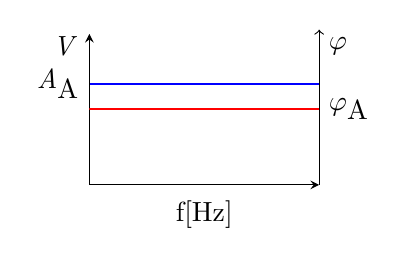
\begin{tikzpicture}[scale=1, transform shape]
    \begin{axis}[
        width=4.5cm, % Breite des Graphen
        height=3.5cm, % Höhe des Graphen
        xmin=0, xmax=10,
        ymin=0, ymax=120,
        axis lines=left,
        axis on top=true,
        domain=0:10,
        xtick=\empty,
        ytick=\empty,
        ylabel style={rotate=270, anchor=east, yshift=0.8cm}, % Position der Beschriftung oben links, horizontal
         ylabel={\it V}, % Hier die gewünschte Beschriftung einfügen
        xlabel={f[Hz]},
        clip mode=individual % Verhindert das Abschneiden von Elementen
        ]
        \addplot+[mark=none, thick, blue] coordinates {(0,80) (10,80)};
        % Adding the left-side label
        \node[anchor=east] at (axis cs:0,80) {$\mathit{A}_{\textnormal{A}}$};
    \end{axis}
    \begin{axis}[
        width=4.5cm, % Breite des Graphen
        height=3.5cm, % Höhe des Graphen
        xmin=0, xmax=10,
        ymin=-180, ymax=180,
        axis y line*=right,
        axis x line=none,
        ytick=\empty,
        ylabel={$\varphi$},
        ylabel style={rotate=270, anchor=west, yshift=0.8cm},
        clip mode=individual, % Verhindert das Abschneiden von Elementen
        after end axis/.code={
            \draw[->] (axis cs:10,180) -- (axis cs:10,190);
        }
        ]
        \addplot+[mark=none, thick, red] coordinates {(0,0) (10,0)};
        \node[anchor=west] at (axis cs:10,0) {$\varphi_{\textnormal{A}}$};
    \end{axis}
    \end{tikzpicture}
\end{center}

\vspace{1ex}
\[
\mathit{a_i} : \text{Amplitude Eingangsspannung i}
\]
\[
\mathit{\varphi_i} : \text{Phase Eingangsspannung i}
\]
\[
\mathit{A}_{A} = \sqrt{a_1^2 + a_2^2 + 2a_1a_2 \cos(\varphi_1 - \varphi_2)}
\]
\[
\mathit{\tan}(\varphi_A) = \frac{a_1 \mathit{\sin}(\varphi_1) + a_2 \mathit{\sin}(\varphi_2)}{a_1 \mathit{\cos}(\varphi_1) + a_2 \mathit{\cos}(\varphi_2)}
\]
\[
    \text{Wenn} : R_2 = R_4 = R
\]
\[
    U_{\textnormal{A}} = (1+ \frac{2R} {R_{\textnormal{g}}}) \cdot \frac{R_3} {R_2} (U_{\textnormal{E2}}-U_{\textnormal{E1}})
\]
     & 
    Differenzverstärker mit hoher Eingangsimpedanz und hoher Gleichtaktunterdrückung  
 \\
    \hline
    \end{tabular}
    \end{table}
    }
\end{frame}

\begin{frame}
    \b{
    \frametitle{Instrumentenverstärker neu}
    \begin{columns}
        \column{0.48\textwidth}
        \centering
        \begin{figure}
    \centering

    \begin{subfigure}{\linewidth}
        \centering
        \resizebox{0.6\linewidth}{!}{\begin{circuitikz}[scale=0.6, transform shape]
    \ctikzset{
         resistors/scale=0.8,              
         tripoles/en amp/height=1.4, % Höhe des OPV             
         tripoles/en amp/width=1.4   % Breite des OPV
    }
    \draw 
    % Erster OPV mit input height=-0.45
    (2,-4.5) node[en amp, noinv input down] (opamp1) {}
    (opamp1.+) --++ (-0.5,0) node[ocirc, label=left:$U_{E2}$] (eingang1) {};
    
   \draw (2,0) node[en amp, noinv input up] (opamp2) {}
    (opamp2.+) --++ (-0.5,0) node[ocirc, label=left:$U_{E1}$] (eingang2) {}
    (opamp1.-)  to[R=$R_g$] (opamp2.-);

   % Dritter OPV mit angepasstem Eingangsabstand
    \ctikzset{tripoles/en amp/input height=0.55} % Anpassung nur für diesen OPV
    \draw (6,-2.25) node[en amp] (opamp3) {}
    (opamp3.-) -- ++(-0.5,0) to[R=$R_1$] ++(-1.5,0) to[R=$R_2$] ++(-2,0) node[circ]{}
    (opamp3.+) -- ++(-0.5,0) to[R=$R_3$] ++(-1.5,0) to[R=$R_4$] ++(-2,0) node[circ]{}
    (opamp2.out) -- ++(0,-1.72) node[circ]{}
    (opamp1.out) -- ++(0,1.72) node[circ]{}
    (opamp3.out) node[circ, label=below:{$U_A$}]{} -- ++(0, 2) to[R=$R_5$] ++(-2,0) -- ++(0, -1.45)node[circ]{};

\end{circuitikz}}
        \caption{Schaltung eines Instrumentenverstärkers}
    \end{subfigure}

    \vspace{0.5cm} 

    \begin{subfigure}{\linewidth}
        \centering
        \resizebox{0.6\linewidth}{!}{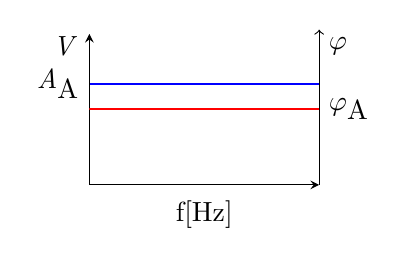
\begin{tikzpicture}[scale=1, transform shape]
    \begin{axis}[
        width=4.5cm, % Breite des Graphen
        height=3.5cm, % Höhe des Graphen
        xmin=0, xmax=10,
        ymin=0, ymax=120,
        axis lines=left,
        axis on top=true,
        domain=0:10,
        xtick=\empty,
        ytick=\empty,
        ylabel style={rotate=270, anchor=east, yshift=0.8cm}, % Position der Beschriftung oben links, horizontal
         ylabel={\it V}, % Hier die gewünschte Beschriftung einfügen
        xlabel={f[Hz]},
        clip mode=individual % Verhindert das Abschneiden von Elementen
        ]
        \addplot+[mark=none, thick, blue] coordinates {(0,80) (10,80)};
        % Adding the left-side label
        \node[anchor=east] at (axis cs:0,80) {$\mathit{A}_{\textnormal{A}}$};
    \end{axis}
    \begin{axis}[
        width=4.5cm, % Breite des Graphen
        height=3.5cm, % Höhe des Graphen
        xmin=0, xmax=10,
        ymin=-180, ymax=180,
        axis y line*=right,
        axis x line=none,
        ytick=\empty,
        ylabel={$\varphi$},
        ylabel style={rotate=270, anchor=west, yshift=0.8cm},
        clip mode=individual, % Verhindert das Abschneiden von Elementen
        after end axis/.code={
            \draw[->] (axis cs:10,180) -- (axis cs:10,190);
        }
        ]
        \addplot+[mark=none, thick, red] coordinates {(0,0) (10,0)};
        \node[anchor=west] at (axis cs:10,0) {$\varphi_{\textnormal{A}}$};
    \end{axis}
    \end{tikzpicture}}
        \caption{Frequenzgang eines Instrumentenverstärkers}
    \end{subfigure}

\end{figure}

        \column{0.48\textwidth}
        \raggedleft
        \begin{itemize}
            \item Gleichung:
         \[
\mathit{a_i} : \text{Amplitude Eingangsspannung i}
\]
\[
\mathit{\varphi_i} : \text{Phase Eingangsspannung i}
\]
\[
\mathit{A}_{A} = \sqrt{a_1^2 + a_2^2 + 2a_1a_2 \cos(\varphi_1 - \varphi_2)}
\]
\[
\mathit{\tan}(\varphi_A) = \frac{a_1 \mathit{\sin}(\varphi_1) + a_2 \mathit{\sin}(\varphi_2)}{a_1 \mathit{\cos}(\varphi_1) + a_2 \mathit{\cos}(\varphi_2)}
\]
\[
    \text{Wenn} : R_2 = R_4 = R
\]
\[
    U_{\textnormal{A}} = (1+ \frac{2R} {R_{\textnormal{g}}}) \cdot \frac{R_3} {R_2} (U_{\textnormal{E2}}-U_{\textnormal{E1}})
\]
        \item Differenzverstärker mit hoher Eingangsimpedanz und hoher Gleichtaktunterdrückung    
    \end{itemize}
    \end{columns}
    }
\end{frame}


%Folie Insutrmentenverstärker 

\begin{frame}
    \b{
        \frametitle{Impedanzwandler}
    \centering
    \begin{table}[ht]
    \label{tab:Impedanzwandler}
    \begin{tabular}{|m{0.24\textwidth}|m{0.405\textwidth}|m{0.25\textwidth}|}
    \hline
    Schaltung & Frequenzgang und Gleichung & Erläuterung und Eigenschaften\\ % Neue Zeile mit Text
    \hline
    \vspace{0.5cm}
    \centering
    \scalebox{0.45}{\begin{circuitikz}
    \ctikzset{tripoles/en amp/input height=0.45}
\draw (0,0)node[en amp, en amp text A](E){}
    (E.out)
    (E.-)
    (E.+);
\draw (E.-) -- (-1.5,0.5) -- (-1.5,2) -- (2,2) to[short,-*] (2,0);
\draw (E.out) to[short, -o] ( 3,0);
\draw (3,-2) to[short, o-o] (-3,-2);
\draw (0,-2)node[ground]{};
\draw (E.+) to[short,-o] (-3,-0.5);


\draw (-3,-0.5) to[open,v>, name=ue] (-3,-2);
\draw (3,0) to[open,v>, name=ua] (3,-2);
\varrmore{ua}{$U_\mathrm{A}$};
\varrmore{ue}{$U_\mathrm{E}$};
\end{circuitikz}}
     &

\vspace{1ex}
Ausgangsspannung $U_\mathrm{A}$ folgt der Eingangsspannung $U_\mathrm{E}$ \newline
Verstärkung $V = \frac{U_\mathrm{A}}{U_\mathrm{E}} = 1$ 

     & 
    
     Auch Spannungsfolger genannt \newline
     Hoher Eingangswiderstand durch Operationsverstärker \newline
     Typische Anwendung: Sensoren

 \\
    \hline
    \end{tabular}
    \end{table}
    }
\end{frame}

\begin{frame}
    \b{
    \frametitle{Impedanzwandler neu}
    \begin{columns}
        \column{0.48\textwidth}
        \centering
        \begin{figure}
        \centering
        \begin{circuitikz}
    \ctikzset{tripoles/en amp/input height=0.45}
\draw (0,0)node[en amp, en amp text A](E){}
    (E.out)
    (E.-)
    (E.+);
\draw (E.-) -- (-1.5,0.5) -- (-1.5,2) -- (2,2) to[short,-*] (2,0);
\draw (E.out) to[short, -o] ( 3,0);
\draw (3,-2) to[short, o-o] (-3,-2);
\draw (0,-2)node[ground]{};
\draw (E.+) to[short,-o] (-3,-0.5);


\draw (-3,-0.5) to[open,v>, name=ue] (-3,-2);
\draw (3,0) to[open,v>, name=ua] (3,-2);
\varrmore{ua}{$U_\mathrm{A}$};
\varrmore{ue}{$U_\mathrm{E}$};
\end{circuitikz}
        \caption{Schaltung eines Impedanzwandlers}

\end{figure}

        \column{0.48\textwidth}
        \centering
        \begin{itemize}
        \item Ausgangsspannung $U_\mathrm{A}$ folgt der Eingangsspannung $U_\mathrm{E}$ 
        \item Verstärkung $V = \frac{U_\mathrm{A}}{U_\mathrm{E}} = 1$ 
        \item Auch Spannungsfolger genannt
        \item Hoher Eingangswiderstand durch Operationsverstärker
        \item Typische Anwendung: Sensoren
    \end{itemize}
    \end{columns}
    }
\end{frame}				%Rückkopplung, Frequenzverhalten und Stabilität
\begin{frame}
    \fta{Stabilität von Verstärkerschaltungen}
    \s{
    Durch die Rückführung des Ausgangssignals auf das Eingangssignal ergibt sich ein Regelkreis. Dieser Regelkreis ist allerdings nicht immer stabil, d.h. die Rückführung führt nicht dazu, dass die Ausgangsgröße sich nur so lange ändert, wie am Eingang auch eine Differenzspannung vorliegt\footnote{Dies ist eine Vereinfachung. In der Regelungstechnik wird zwischen Lyapunov-Stabilität und BIBO-Stabilität unterschieden (siehe hierzu z.B. \glqq Regelungstechnik\grqq{} von Otto Föllinger)}.
    Dies wird deutlich, wenn das Ausgangssignal auf den nicht-invertierenden anstatt den invertierenden Eingang zurückgeführt wird. Wird nun eine Spannungssdifferenz an den Eingang angelegt und am Ausgang verstärkt ausgegeben, so führt diese Ausgangsspannung zu einer erneuten Erhöhung der Spannungsdifferenz am Eingang. 
    Das System ist also nicht stabil. Ein ähnliches Phänomen kann beobachtet werden, wenn in der Verstärkerschaltung Energiespeicher (Kondensatoren oder Spulen) verwendet werden. Eine solche Schaltung weißt immer eine Stabilitätsgrenze auf, die dann erreicht wird, wenn das auf den invertierenden Eingang rückgekoppelte Signal, eine Phasenverschiebung von 180$^{\circ}$ aufweist.
    In diesem Fall wird die Gegenkopplung zur Mitkopplung und die Schaltung wird instabil. 
    Das ist aber nicht die einzige Möglichkeit, wie eine Schaltung instabil werden kann. Auch kann die Schaltung ins Schwingen geraten, wenn die Energiespeicher nicht richtig dimensioniert werden. Aus diesem Grund sind Stabilitätsanalysen der entworfenen Schaltungen unerlässlich. 
    
    Es sollen im Rahmen dieses Kapitels folgende Kompetenzen erworben werden:


%\speech{1}{
%    Stabilität von Verstärkerschaltungen
%    Durch die Rückführung des Ausgangssignals auf das Eingangssignal ergibt sich ein Regelkreis. Dieser Regelkreis ist allerdings nicht immer stabil, d.h. die Rückführung führt nicht dazu, dass die Ausgangsgröße sich nur so lange ändert, wie am Eingang auch eine Differenzspannung vorliegt\footnote{Dies ist eine Vereinfachung. In der Regelungstechnik wird zwischen Lyapunov-Stabilität und BIBO-Stabilität unterschieden (siehe hierzu z.B. \glqq Regelungstechnik\grqq{} von Otto Föllinger)}.
%    Dies wird deutlich, wenn das Ausgangssignal auf den nicht-invertierenden anstatt den invertierenden Eingang zurückgeführt wird. Wird nun eine Spannungssdifferenz an den Eingang angelegt und am Ausgang verstärkt ausgegeben, so führt diese Ausgangsspannung zu einer erneuten Erhöhung der Spannungsdifferenz am Eingang.
%    Das System ist also nicht stabil. Ein ähnliches Phänomen kann beobachtet werden, wenn in der Verstärkerschaltung Energiespeicher (Kondensatoren oder Spulen) verwendet werden. Eine solche Schaltung weißt immer eine Stabilitätsgrenze auf, die dann erreicht wird, wenn das auf den invertierenden Eingang rückgekoppelte Signal, eine Phasenverschiebung von 180$^{\circ}$ aufweist.
%    In diesem Fall wird die Gegenkopplung zur Mitkopplung und die Schaltung wird instabil.
%    Das ist aber nicht die einzige Möglichkeit, wie eine Schaltung instabil werden kann. Auch kann die Schaltung ins Schwingen geraten, wenn die Energiespeicher nicht richtig dimensioniert werden. Aus diesem Grund sind Stabilitätsanalysen der entworfenen Schaltungen unerlässlich.
%    Es sollen im Rahmen dieses Kapitels folgende Kompetenzen erworben werden:
%}
    \s{
        \begin{Lernziele}{Operationsverstärker}
            \title{Lernziele: Stabilität von Verstärkerschaltungen}
            Die Studierenden können
            \begin{itemize}
                \item Stabilitätsanalysen durchführen und Ergebnisse der Analyse beurteilen.
                \item Bauteile in OPV-Schaltungen dem Stabilitätskriterien entsprechend dimensionieren.
            \end{itemize}
        \end{Lernziele}
    }
    

%\speech{1}{
%    Lernziele
%    Die Studierenden können Stabilitätsanalysen durchführen und Ergebnisse der Analyse beurteilen. Sie können Bauteile in OPV-Schaltungen dem Stabilitätskriterien entsprechend dimensionieren.
%}
    Einige der Stabilitätskriterien, die zur Stabilitätsbewertung herangezogen werden sind im Folgenden beschrieben.
    Die Bewertung der Stabilität von Operationsverstärkerschaltungen ist eine wichtige Fähigkeit für Studierende der Elektrotechnik, egal ob die Schaltungen von Grund auf entworfen oder Fehler in bestehenden Schaltungen behoben werden sollen. 
    Diese Bewertung stellt sicher, dass Operationsverstärkerschaltungen zuverlässig und effektiv arbeiten, was für ihre Integration in verschiedene elektronische Systeme unerlässlich ist. Im Folgenden wird erläutert, welche Methoden zur Bewertung der Stabilität verwendet werden.

   %\speech{1}{
   % Einige der Stabilitätskriterien, die zur Stabilitätsbewertung herangezogen werden sind im Folgenden beschrieben.
   % Die Bewertung der Stabilität von Operationsverstärkerschaltungen ist eine wichtige Fähigkeit für Studierende der Elektrotechnik, egal ob die Schaltungen von Grund auf entworfen oder Fehler in bestehenden Schaltungen behoben werden sollen. 
   % Diese Bewertung stellt sicher, dass Operationsverstärkerschaltungen zuverlässig und effektiv arbeiten, was für ihre Integration in verschiedene elektronische Systeme unerlässlich ist. 
   % Im Folgenden wird erläutert, welche Methoden zur Bewertung der Stabilität verwendet werden.
   % }
   } 
	\b{\frametitle{Stabilität des Operationsverstärker-Regelkreis}
    Durch die Rückführung des Ausgangssignal ergibt sich ein Regelkreis. Dieser muss auf Stabilität überprüft werden. Dazu werden 3 Methoden vorgstellt:
    \begin{itemize}
    \item Die Frequengangzanalyse auf Grundlage des Bodediagramms
    \item Die Untersuchung der Übertragungsfunktion auf ihre Pollagen
    \item Die Analyse des Einschwingverhaltens
    \end{itemize}}
\end{frame}

%Frequenzganganalyse
\begin{frame}
    \frametitle{Frequenzgangsanalyse (experimentell/simulativ)}
    \s{
    Eine grundlegende Technik ist die Frequenzganganalyse. 
    Bei diesem Verfahren wird untersucht, wie sich die Verstärkung und die Phase einer Operationsverstärkerschaltung ändern, wenn die Frequenz des Eingangssignals variiert. Werkzeuge wie Bodediagramme werden häufig zur Visualisierung dieser Reaktion eingesetzt und helfen bei der Identifizierung potenzieller Stabilitätsprobleme wie Verstärkungsspitzen oder Phasenverschiebungen, die zu Instabilität führen könnten.
    Ein wichtiges Kriterium bildet hier die Phasenreserve. Die Bestimmung dieser Größe ist ein quantitativer Ansatz zur Stabilitätsbewertung. Sie hilft bei der Messung der Stabilitätsspanne innerhalb eines Rückkopplungssystems, indem sie die Phasendifferenz zwischen der tatsächlichen Phasenverschiebung bei der Durchtrittsfrequenz (also 0 dB) und 180$^{\circ}$ betrachtet. Dieser Punkt wird als \glqq kritischer Punkt\grqq{} bezeichnet, da bei einer Phasenverschiebung über 180$^{\circ}$ und einer Verstärkung über 0 dB, die Rückkopplung zur Mitkopplung wird. 
    Wenn die Phasendifferenz einen bestimmten Schwellenwert überschreitet, in der Regel etwa 45$^{\circ}$, wird davon ausgegangen, dass das System weit genug von der Stabilitätsgrenze entferent ist.
    Diese Analyse findet normalerweise graphisch auf Grundlage des Bodediagramms statt. 
    }
        \begin{center}
        \b{Bei dieser Methode wird das Bodediagramm im relevanten Frequenzbereich betrachtet.} 
        \f{width=\textwidth}{width=0.9\textwidth}{Bilder/kap4/Amplitudengang Regelkreis und Phasengang.pdf}{Bestimmung der Phasenreserve auf Grundlage des Bodediagramms} 
        \label{fig:Frequenzganganalyse}
    \end{center}
    \b{Auf dieser Grundlage wird die Phasenlage am 0 dB-Durchtrittspunkt der Amplitude bestimmt. Besteht ein geringer Abstand zu -180° ist das System instabil.}  %Inspiration: https://www.google.com/search?client=firefox-b-d&sca_esv=07fc2a91d39bc3b9&sca_upv=1&sxsrf=ADLYWIJlgSTFsuVgmDjND0631smrCLZH5g:1720507056816&q=phasenreserve&udm=2&fbs=AEQNm0A6bwEop21ehxKWq5cj-cHa02QUie7apaStVTrDAEoT1A_pRBhSGXWPGL0_xk71SHFUmHSJWGPXoD9Kj5_rnHbWMOqF2geje-KRnle5TYvzlu3NqubtU_abXJaIrzdDTfJXR1IEap8k1YruTZC6a9-SgzP6gSnzb0vwoljHMAsMGnOtcGrx634vR4spXb0931ZlkiFj&sa=X&ved=2ahUKEwjcztGfrJmHAxUygP0HHerJD6MQtKgLegQIDRAB&biw=1536&bih=835&dpr=1.25#vhid=kWaDK2aKHZdoUM&vssid=mosaic         
    
\end{frame}

%\speech {1}{ Frequenzganganalyse
%    Eine grundlegende Technik ist die Frequenzganganalyse. Bei diesem Verfahren wird untersucht, wie sich die Verstärkung und die Phase einer Operationsverstärkerschaltung ändern, wenn die Frequenz des Eingangssignals variiert. Werkzeuge wie Bodediagramme werden häufig zur Visualisierung dieser Reaktion eingesetzt und helfen bei der Identifizierung potenzieller Stabilitätsprobleme wie Verstärkungsspitzen oder Phasenverschiebungen, die zu Instabilität führen könnten.
%    Ein wichtiges Kriterium bildet hier die Phasenreserve. Die Bestimmung dieser Größe ist ein quantitativer Ansatz zur Stabilitätsbewertung. Sie hilft bei der Messung der Stabilitätsspanne innerhalb eines Rückkopplungssystems, indem sie die Phasendifferenz zwischen der tatsächlichen Phasenverschiebung bei der Durchtrittsfrequenz (also 0 dB) und 180$^{\circ}$ betrachtet. Dieser Punkt wird als \glqq kritischer Punkt\grqq{} bezeichnet, da bei einer Phasenverschiebung über 180$^{\circ}$ und einer Verstärkung über 0 dB, die Rückkopplung zur Mitkopplung wird. 
%    Wenn die Phasendifferenz einen bestimmten Schwellenwert überschreitet, in der Regel etwa 45$^{\circ}$, wird davon ausgegangen, dass das System weit genug von der Stabilitätsgrenze entferent ist.
%    Diese Analyse findet normalerweise graphisch auf Grundlage des Bodediagramms statt. 
%}
%\speech{
%Abbildung 4.1 zeigt die Bestimmung der Phasenreserve anhand eines Bode-Diagramms.  
%Das Diagramm besteht aus zwei Graphen.  
%Der obere Graph stellt den Amplitudengang dar, der untere Graph zeigt den Phasengang.  
%Die x-Achse repräsentiert die Frequenz des Systems.  
%
%Im oberen Graphen ist die Amplitude des offenen Regelkreises dargestellt.  
%Die Amplitude nimmt mit steigender Frequenz ab.  
%Die Durchtrittsfrequenz ist als Schnittpunkt mit der Null-Dezibel-Linie markiert.  
%
%Im unteren Graphen ist der Phasengang des offenen Regelkreises dargestellt.  
%Die Phase beginnt bei null Grad und nimmt mit steigender Frequenz ab.  
%Sie nähert sich minus 180 Grad an.  
%Die Phasenreserve ist der Abstand zwischen der tatsächlichen Phasenverschiebung bei der Durchtrittsfrequenz und der Marke von minus 180 Grad.  
%
%Eine hohe Phasenreserve bedeutet, dass das System stabil ist.  
%Eine geringe oder negative Phasenreserve führt zu Instabilität oder Schwingungen im Regelkreis.  
%
%Dieses Diagramm wird verwendet, um die Stabilität von Regelkreisen zu analysieren.  
%}

%Analyse der Übertragungsfunktion
\begin{frame}
    \frametitle{Analyse der Übertragungsfunktion (analytisch)}
    \s{
    \par
    Liegt die Übertragungsfunktion der Operationsverstärkerschaltung vor, kann auch direkt eine Stabilitätsanalyse durchgeführt werden. Dazu werden die Pole der Übertragungsfunktion (z.B. im Laplacebereich) analysiert. Liegen diese in der linken s-Halbebene (also sind alle Pole negativ), weißt die Schaltung ein stabiles Übertragungsverhalten auf.
    Bei diesem Ansatz sowie bei der Frequnzanalyse (sofern das Bodediagramm nicht experimentell ermittelt wurde) muss beachtet werden, dass die Übertragungsfunktion meist nur für einen bestimmten Frequenzbereich gültig ist, da z.B. die Dynamik des Operationsverstärkers bei diesen Methoden in der Regel nicht berücksichtigt wird.
    \begin{center}
        %\input{Bilder/kap4/Filter.png}
        \f{width=0.8\textwidth}{width=0.8\textwidth}{Bilder/kap4/Polstellenneu.pdf}{Systemantworten bei verschiedenen Pollagen }
        \label{fig:Analyse des Schwingungsverhaltens}             
    \end{center}
    }
%    \b{Bei dieser Methode wird werden die Polstellen der Übertragunsfunktion bestimmt. Unten ist dargestellt, welches %Ausgangsverhalten bei welchen Pollagen erwartet werden kann.
%        \begin{center}
%        %\input{Bilder/kap4/Filter.png}
%        \f{width=1\textwidth}{width=0.5\textwidth}{Bilder/kap4/Polstellenneu.pdf}{Systemantworten bei verschiedenen Pollagen \cite%{Kolahi}}
%        \label{fig:Analyse des Schwingungsverhaltens}             
%    \end{center}
%    }
\end{frame}

%\speech{1}{
%   Analyse der Übertragungsfunktion
%   Liegt die Übertragungsfunktion der Operationsverstärkerschaltung vor, kann auch direkt eine Stabilitätsanalyse durchgeführt werden. Dazu werden die Pole der Übertragungsfunktion (z.B. im Laplacebereich) analysiert. Liegen diese in der linken s-Halbebene (also sind alle Pole negativ), weißt die Schaltung ein stabiles Übertragungsverhalten auf.
%   Bei diesem Ansatz sowie bei der Frequnzanalyse (sofern das Bodediagramm nicht experimentell ermittelt wurde) muss beachtet werden, dass die Übertragungsfunktion meist nur für einen bestimmten Frequenzbereich gültig ist, da z.B. die Dynamik des Operationsverstärkers bei diesen Methoden in der Regel nicht berücksichtigt wird.
%}

%\speech{
%Abbildung 4.2 zeigt die Systemantworten für verschiedene Pol-Lagen in der komplexen Zahlenebene.  
%Die x-Achse stellt die Realachse dar, die y-Achse die Imaginärachse.  
%Verschiedene Pole sind mit farbigen Symbolen markiert, und neben jedem Pol ist die entsprechende Systemantwort als Zeitverlauf dargestellt.  
%
%Negative reelle Pole befinden sich auf der linken Seite der x-Achse.  
%Die zugehörigen Systemantworten zeigen exponentiell abklingende Signale.  
%Je weiter links der Pol liegt, desto schneller erfolgt das Abklingen.  
%
%Positive reelle Pole befinden sich auf der rechten Seite der x-Achse.  
%Diese führen zu exponentiell wachsenden Signalen, was auf ein instabiles System hinweist.  
%
%Komplex konjugierte Pole mit negativem Realteil liegen in der linken oberen und unteren Hälfte des Diagramms.  
%Die zugehörigen Systemantworten zeigen gedämpfte Schwingungen.  
%Je weiter links der Pol liegt, desto stärker ist die Dämpfung.  
%
%Komplex konjugierte Pole mit positivem Realteil befinden sich in der rechten oberen und unteren Hälfte.  
%Diese führen zu verstärkten, instabilen Schwingungen mit zunehmender Amplitude.  
%
%Reine imaginäre Pole liegen entlang der y-Achse.  
%Die zugehörigen Systemantworten zeigen ungedämpfte Schwingungen mit konstanter Amplitude.  
%
%Ein Pol im Ursprung führt zu einer Systemantwort mit einer konstanten Verschiebung oder einem linearen Anstieg.  
%
%Diese Abbildung zeigt, wie die Position der Pole in der komplexen Ebene das dynamische Verhalten eines Systems bestimmt.  
%Stabile Systeme haben alle Pole in der linken Halbebene.  
%Instabile Systeme besitzen mindestens einen Pol mit positivem Realteil.  
%}


%Analyse der Einschwingverhaltens
\begin{frame}
    \pagebreak
    \frametitle{Analyse des Einschwingverhaltens (experimentell/simulativ)}
    \s{
    \par
    Eine weitere wichtige Methode ist die Analyse des Einschwingverhaltens. Bei dieser Methode wird ein Spannungssprung auf die Verstärkerschaltung gegeben um zu untersuchen, wie eine Operationsverstärkerschaltung auf plötzliche Änderungen der Eingangssignale reagiert. Durch Beobachtung der Reaktion des Schaltkreises kann so eine Aussage getroffen werden, ob das System zur Instabilität neigt. In der Realität ist dieser Test sehr vorsichtig durchzuführen, da bei 
    bei einer instabilen Schaltung schnell Bauteile zerstört werden können. Aus diesem Grund wird ein solcher Test heutzutage häufig rein simulativ durchgeführt. Als Faustregel lässt sich hier sagen: Wenn die Schaltung nach einer Anregung durch einen Einheitssprung gegen einen festen Wert strebt und keine Dauerschwingung ausführt, kann das Einschwingverhalten als stabil angenommen werden.
    }

    \b{Bei dieser Methode wird die Schaltung mit einem Eingangssignal angeregt und das Ausgangsverhalten beobachtet.} 
        \begin{center}
        %\input{Bilder/kap4/Filter.png}
        \f{width=0.8\textwidth}{width=0.8\textwidth}{Bilder/kap4/ubertragunsverhalten-Einschwingverhalten.pdf}{Stabiles und instabiles Einschwingverhalten} %https://link.springer.com/chapter/10.1007/978-3-662-64375-4_52  
        \label{fig:Einschwingverhalten}             
    \end{center}
    \s{
        Wie dargestellt wurde, ist die Stabilitätsanalyse ein komplexes Thema und soll hier nur angeschnitten werden. An dieser Stelle wird kein Wert auf Vollständigkeit gelegt. 
        Die genannten Analysemethoden sind Teil der Regelungstechnik und in der einschlägigen Literatur nachzulesen.

        \begin{Merksatz}{}
            Durch die Rückführung des Ausgangssignal auf den Eingang ergibt sich ein Regelkreis.
            Die Stabilität dieses Regelkreises muss simulativ, experimentell oder analytisch überprüft werden. 
        \end{Merksatz}
    }
\end{frame}

%\speech {1}{
%    Analyse des Einschwingverhaltens
%    Eine weitere wichtige Methode ist die Analyse des Einschwingverhaltens. Bei dieser Methode wird ein Spannungssprung auf die Verstärkerschaltung gegeben um zu untersuchen, wie eine Operationsverstärkerschaltung auf plötzliche Änderungen der Eingangssignale reagiert. Durch Beobachtung der Reaktion des Schaltkreises kann so eine Aussage getroffen werden, ob das System zur Instabilität neigt. In der Realität ist dieser Test sehr vorsichtig durchzuführen, da bei 
%    bei einer instabilen Schaltung schnell Bauteile zerstört werden können. Aus diesem Grund wird ein solcher Test heutzutage häufig rein simulativ durchgeführt. Als Faustregel lässt sich hier sagen: Wenn die Schaltung nach einer Anregung durch einen Einheitssprung gegen einen festen Wert strebt und keine Dauerschwingung ausführt, kann das Einschwingverhalten als stabil angenommen werden.
%    Wie dargestellt wurde, ist die Stabilitätsanalyse ein komplexes Thema und soll hier nur angeschnitten werden. An dieser Stelle wird kein Wert auf Vollständigkeit gelegt.
%    Die genannten Analysemethoden sind Teil der Regelungstechnik und in der einschlägigen Literatur nachzulesen.
%}
%\speech{
%Abbildung 4.3 zeigt das Einschwingverhalten eines Systems in zwei unterschiedlichen Fällen.  
%Das linke Diagramm zeigt stabiles Verhalten, das rechte Diagramm zeigt instabiles Verhalten.  
%Beide Diagramme stellen den zeitlichen Verlauf der Ausgangsgröße U A in Abhängigkeit von der Zeit t dar.  
%
%Im linken Diagramm für stabiles Verhalten beginnt die Ausgangsspannung mit einer schnellen Änderung.  
%Es gibt eine Überschwingung, gefolgt von einer gedämpften Schwingung.  
%Nach einer kurzen Einschwingzeit erreicht die Spannung einen stationären Endwert,  
%der durch eine gestrichelte Linie dargestellt ist.  
%Das System verhält sich stabil, weil es sich nach kurzer Zeit beruhigt.  
%
%Im rechten Diagramm für instabiles Verhalten beginnt die Ausgangsspannung ebenfalls mit einer schnellen Änderung.  
%Jedoch bleiben die Schwingungen bestehen und nehmen im Verlauf der Zeit nicht ab.  
%Die Amplitude der Schwingung nimmt nicht ab oder wächst sogar.  
%Das bedeutet, dass das System nicht zur Ruhe kommt und instabil bleibt.  
%
%Zusammenfassung:  
%Ein stabiles System erreicht nach einer gewissen Zeit einen stationären Zustand.  
%Ein instabiles System zeigt wachsende oder andauernde Schwingungen.  
%Dies ist ein wichtiger Aspekt bei der Stabilitätsanalyse von Regelkreisen.  
%}
				%Operationsverstärkerschaltungen und Anwendungsgebiete
\begin{frame}
    \fta{Operationsverstärker als Analogrechner}
    \s{
    Neben dem Einsatz von Operationsverstärkern in Messverstärkern, werden OPVs auch in Analogrechnern eingesetzt.
    Das mag in der Zeit hochperformanter Prozessoren nicht mehr relevant wirken, hat aber durchaus Vorteile. So kann die Berechnungszeit mithilfe von Operationsverstärkern deutlich reduziert werden.
    Das macht vor allem in Anwendungen Sinn, in denen nur eine Rechenoperation (Multiplikation, Addition o.ä.) durchgeführt werden soll, aber so gut wie keine Latenzen auftreten dürfen.
    Dies ist heutzutage noch häufig in der Regelungstechnik der Fall. 
    
    Es sollen im Rahmen dieses Kapitels folgende Kompetenzen erworben werden:
    \s{
        \begin{Lernziele}{Operationsverstärker}
            \title{Lernziele: Operationsverstärker als Analogrechner}
            Die Studierenden können
            \begin{itemize}
                \item geeignete Operationsverstärkerschaltungen für eine Problemlösung angegeben.
                \item Widerstandsverhältnisse berechnen.
            \end{itemize}
        \end{Lernziele}
    }
%\speech{Operationsverstärker als Analogrechner}{1}{
%    Neben dem Einsatz von Operationsverstärkern in Messverstärkern, werden OPVs auch in Analogrechnern eingesetzt.
%    Das mag in der Zeit hochperformanter Prozessoren nicht mehr relevant wirken, hat aber durchaus Vorteile. So kann die Berechnungszeit mithilfe von Operationsverstärkern deutlich reduziert werden.
%    Das macht vor allem in Anwendungen Sinn, in denen nur eine Rechenoperation (Multiplikation, Addition o.ä.) durchgeführt werden soll, aber so gut wie keine Latenzen auftreten dürfen.
%    Dies ist heutzutage noch häufig in der Regelungstechnik der Fall.
%    Es sollen im Rahmen dieses Kapitels folgende Kompetenzen erworben werden:
%}

%\speech{Lernziele: Operationsverstärker als Analogrechner}{1}{
%    Die Studierenden können geeignete Operationsverstärkerschaltungen für eine Problemlösung angeben und Widerstandsverhältnisse berechnen. 
%    Sie können mithilfe von Operationsverstärkerschaltungen einen Analogrechner aufbauen und die Funktionsweise erklären.
%}
    Im Folgenden sollen ein Beispiel vorgestellt werden, das zeigen soll, wie mithilfe der in der Tabelle gegebenen Operationsverstärkergrundschaltungen 
    ein Analogrechner aufgebaut werden kann.

    \begin{bsp}{Beispiel Analogrechner}{Beispiel Analogrechner}
        Es soll eine Schaltung entworfen werden, die folgende Funktion umsetzt:
        \begin{equation}
            U_{\textnormal{A}} = \int U_{\textnormal{E1}} dt +x \cdot U_{\textnormal{E1}} - 2\cdot U_{\textnormal{E2}} 
        \end{equation}
        
        \textbf{Lösung}\\
        Zunächst muss die Gleichung in zwei Teilprobleme zerlegt werden, die mithilfe von Operationsverstärkerschaltungen gelöst werden können.
        Das erste Teilproblem bildet die Integration des Eingangssignals $U_{E1}$. Dazu soll zunächst eine Integratorschaltung verwendet werden.
        Das zweite Teilproblem bildet die Addition der Signale. Dafür kann ein Summierer verwendet werden.
        Durch eine Kombination von einer Integratorschaltung und einem Summierer ist also das gewünschte Verhalten zu erreichen. Ist es mit dieser Schaltung möglich x=0 zu wählen?
        
            \fu{
            \resizebox{0.6\textwidth}{!}{\begin{circuitikz}[scale=0.7, transform shape]
    \ctikzset{
              resistors/scale=0.8,              
              tripoles/en amp/height=1.4, % Höhe des OPV             
              tripoles/en amp/width=1.4,   % Breite des OPV
             capacitors/scale=0.5,
             tripoles/en amp/input height=0.45
    }
         \fill[yellow, opacity=0.2] (-3.1,-1.2) rectangle (1.1,3.5);
         \fill[violet, opacity=0.2] (1.6,-1.6) rectangle (7,2.5);
         \draw[yellow, thick] (-3.1,-1.2) rectangle (1.1,3.5);
         \draw[violet, thick] (1.6,-1.6) rectangle (7,2.5);

         \draw (0,0) node[en amp] (opamp) {}
         (opamp.+) --++ (-0.5,0) node[ground] {} 
         (opamp.-) -- ++(0, 0) to[R, l_=$R_1$] ++(-1.2, 0) node[ocirc, label=left:$U_{E1}$] {}
         (opamp.out) node[circ] {} -- ++(0,1.5) to[C, l_=$C$, *-] ++(-1.9,0) node[circ]{}
         (opamp.out) node[circ] {} -- ++(0,2.8) to[R, l_=$R_2$] ++(-1.9,0) -- ++(0, -2.35) node[circ] {};

        \draw
        (5,-0.45) node[en amp] (opamp2) {}
        (opamp.out) -- ++(1.6,0) to[R, l=$R_3$, -*] (opamp2.-) 
        (opamp2.+)  node[ground] {}
        (opamp2.-) |- ++(0,1) to[R, l=$R_5$] ++(1.9,0) -| (opamp2.out)
        (opamp2.-) -- ++(0,-0.5) -- ++(-0.0,0) to[R, l=$R_4$] ++(-1.438,0) node[ocirc, label=left:$U_{E2}$] {}
        (opamp2.out) to[short, *-o] ++(0.2,0) node[right] {$U_{A}$};

\end{circuitikz}


    


}
            }{Schaltung zur Lösung der Analogrechneraufgabe
            \label{fig:Analogrechner}}

        \begin{equation}
            U_{\textnormal{A}} = \underbrace{\left[ -\frac{1}{R_1 \cdot C} \int_{0}^{t} U_{\textnormal{E1}}~dt -\frac{R_2}{R_1} \cdot U_{\textnormal{E1}} \right]}_{Formel~des~Integrators} \underbrace{\cdot\left(-\frac{R_5}{R_3}\right)-\frac{R_5}{R_4}\cdot U_{\textnormal{E2}}}_{Formel~des~Summierers} 
        \end{equation}
        Dies kann nun wie folgt umgeformt werden
        \begin{equation}
            U_{\textnormal{A}} = \underbrace{\frac{R_5}{R_1 \cdot R_3 \cdot C}}_{\stackrel{!}{=}1} \int_{0}^{t} U_{\textnormal{E1}}~dt + \underbrace{\frac{R_2 R_5}{R_1 R_3}}_{\stackrel{!}{=}x} U_{\textnormal{E1}} -\underbrace{\frac{R_5}{R_4}}_{\stackrel{!}{=}2} \cdot U_{\textnormal{E2}} 
        \end{equation}

        Wie der Formel zu entnehmen ist, müssen nun die Bauteilwerte nur noch so gewählt werden, dass sich die richtigen Vorfaktoren ergeben.
        Eine Wahl von x=0 ist nur möglich, wenn der Widerstand $R_2$ weggelassen wird. In diesem Fall ergibt sich ein \glqq idealer\grqq{}, der in der Realität so allerdings in der Regel nicht aufgebaut wird. 

    \end{bsp}
   %% \f{width=1\textwidth}{width=\textwidth}{kap5/Analogrechner.tex}{Schaltung zur Lösung der Analogrechneraufgabe \label{fig:Analogrechner Skript}} 


    }
	\b{\frametitle{Operationsverstärker als Analogrechner}
        Es soll eine Schaltung entworfen werden, die folgende Funktion umsetzt:
        \begin{equation}
            U_{\textnormal{A}} = \int U_{\textnormal{E1}} +x \cdot U_{\textnormal{E1}} - 2\cdot U_{\textnormal{E2}} 
        \end{equation}

        Wie kann das erreicht werden? Überlegen Sie sich zunächst, welche Grundschaltungen hierfür zu kombinieren sind. 
        }
\end{frame}

\begin{frame}
    \b{
        \frametitle{Lösungsschritt 1: Verstärkerschaltung}
        Zunächst muss die obere Gleichung in zwei Teilprobleme zerlegt werden, die mithilfe von Operationsverstärkerschaltungen gelöst werden können.
        Das erste Teilproblem bildet die Integration des Eingangssignals $U_{E1}$. Dazu soll zunächst eine Integratorschaltung verwendet werden.
        Das zweite Teilproblem bildet die Addition der Signale. Dafür kann ein Summierer verwendet werden.
        \begin{figure}[ht]
            \centering
            \fu{
            \resizebox{0.7\textwidth}{!}{\begin{circuitikz}[scale=0.7, transform shape]
    \ctikzset{
              resistors/scale=0.8,              
              tripoles/en amp/height=1.4, % Höhe des OPV             
              tripoles/en amp/width=1.4,   % Breite des OPV
             capacitors/scale=0.5,
             tripoles/en amp/input height=0.45
    }
         \fill[yellow, opacity=0.2] (-3.1,-1.2) rectangle (1.1,3.5);
         \fill[violet, opacity=0.2] (1.6,-1.6) rectangle (7,2.5);
         \draw[yellow, thick] (-3.1,-1.2) rectangle (1.1,3.5);
         \draw[violet, thick] (1.6,-1.6) rectangle (7,2.5);

         \draw (0,0) node[en amp] (opamp) {}
         (opamp.+) --++ (-0.5,0) node[ground] {} 
         (opamp.-) -- ++(0, 0) to[R, l_=$R_1$] ++(-1.2, 0) node[ocirc, label=left:$U_{E1}$] {}
         (opamp.out) node[circ] {} -- ++(0,1.5) to[C, l_=$C$, *-] ++(-1.9,0) node[circ]{}
         (opamp.out) node[circ] {} -- ++(0,2.8) to[R, l_=$R_2$] ++(-1.9,0) -- ++(0, -2.35) node[circ] {};

        \draw
        (5,-0.45) node[en amp] (opamp2) {}
        (opamp.out) -- ++(1.6,0) to[R, l=$R_3$, -*] (opamp2.-) 
        (opamp2.+)  node[ground] {}
        (opamp2.-) |- ++(0,1) to[R, l=$R_5$] ++(1.9,0) -| (opamp2.out)
        (opamp2.-) -- ++(0,-0.5) -- ++(-0.0,0) to[R, l=$R_4$] ++(-1.438,0) node[ocirc, label=left:$U_{E2}$] {}
        (opamp2.out) to[short, *-o] ++(0.2,0) node[right] {$U_{A}$};

\end{circuitikz}


    


}
            }{Schaltung zur Lösung der Analogrechneraufgabe
            \label{fig:Analogrechner2}}
        \end{figure}
        Durch eine Kombination von einer Integratorschaltung und einem Summierer ist also das gewünschte Verhalten zu erreichen. Ist es mit dieser Schaltung möglich x=0 zu wählen?
        }
\end{frame}

\begin{frame}
    \b{   
        \frametitle{Lösungsschritt 2: Rechnung}
       
        \begin{equation}
            U_{\textnormal{A}} = \underbrace{\left[ -\frac{1}{R_1 \cdot C} \int_{0}^{t} U_{\textnormal{E1}}~dt -\frac{R_2}{R_1} \cdot U_{\textnormal{E1}} \right]}_{Formel~des~Integrators} \underbrace{\cdot\left(-\frac{R_5}{R_3}\right)-\frac{R_5}{R_4}\cdot U_{\textnormal{E2}}}_{Formel~des~Summierers} 
        \end{equation}
        Dies kann nun wie folgt umgeformt werden
        \begin{equation}
            U_{\textnormal{A}} = \underbrace{\frac{R_5}{R_1 \cdot R_3 \cdot C}}_{\stackrel{!}{=}1} \int_{0}^{t} U_{\textnormal{E1}}~dt + \underbrace{\frac{R_2 R_5}{R_1 R_3}}_{\stackrel{!}{=}x} U_{\textnormal{E1}} -\underbrace{\frac{R_5}{R_4}}_{\stackrel{!}{=}2} \cdot U_{\textnormal{E2}} 
        \end{equation}

        Wie der Formel zu entnehmen ist, müssen nun die Bauteilwerte nur noch so gewählt werden, dass sich die richtigen Vorfaktoren ergeben.
        Eine Wahl von x=0 ist nur möglich, wenn der Widerstand $R_2$ weggelassen wird. 
    }
\end{frame}

%\speech{Beispiel 5.1: Beispiel Analogrechner}{1}{
%    Es soll eine Schaltung entworfen werden, die folgende Funktion umsetzt:
%    \begin{equation}
%        U_{\textnormal{A}} = \int U_{\textnormal{E1}} dt +x \cdot U_{\textnormal{E1}} - 2\cdot U_{\textnormal{E2}}
%    \end{equation}
%    Lösung: Zunächst muss die Gleichung in zwei Teilprobleme zerlegt werden, die mithilfe von Operationsverstärkerschaltungen gelöst werden können.
%    Das erste Teilproblem bildet die Integration des Eingangssignals $U_{E1}$. Dazu soll zunächst eine Integratorschaltung verwendet werden.
%    Das zweite Teilproblem bildet die Addition der Signale. Dafür kann ein Summierer verwendet werden.
%    Durch eine Kombination von einer Integratorschaltung und einem Summierer ist also das gewünschte Verhalten zu erreichen. Ist es mit dieser Schaltung möglich x=0 zu wählen?
%   
%    \begin{equation}
%        U_{\textnormal{A}} = \underbrace{\left[ -\frac{1}{R_1 \cdot C} \int_{0}^{t} U_{\textnormal{E1}}~dt -\frac{R_2}{R_1} \cdot U_{\textnormal{E1}} \right]}_{Formel~des~Integrators} \underbrace{\cdot\left(-\frac{R_5}{R_3}\right)-\frac{R_5}{R_4}\cdot U_{\textnormal{E2}}}_{Formel~des~Summierers} 
%    \end{equation}
%    Dies kann nun wie folgt umgeformt werden
%    \begin{equation}
%        U_{\textnormal{A}} = \underbrace{\frac{R_5}{R_1 \cdot R_3 \cdot C}}_{\stackrel{!}{=}1} \int_{0}^{t} U_{\textnormal{E1}}~dt + \underbrace{\frac{R_2 R_5}{R_1 R_3}}_{\stackrel{!}{=}x} U_{\textnormal{E1}} -\underbrace{\frac{R_5}{R_4}}_{\stackrel{!}{=}2} \cdot U_{\textnormal{E2}} 
%    \end{equation}
%
%    Wie der Formel zu entnehmen ist, müssen nun die Bauteilwerte nur noch so gewählt werden, dass sich die richtigen Vorfaktoren ergeben.
%    Eine Wahl von x=0 ist nur möglich, wenn der Widerstand $R_2$ weggelassen wird. In diesem Fall ergibt sich ein \glqq idealer\grqq{}, der in der Realität so allerdings in der Regel nicht aufgebaut wird.   
%}
%\speech{
%Abbildung 5.1 zeigt eine elektronische Schaltung zur Lösung einer Analogrechneraufgabe. Die Schaltung ist in zwei farblich gekennzeichnete Bereiche unterteilt: einen gelben Bereich links und einen violetten Bereich rechts.
%
%Im linken Bereich befindet sich ein Operationsverstärker mit einer Rückkopplungsschleife, die aus einem Widerstand und einem Kondensator besteht. Der nicht-invertierende Eingang des Operationsverstärkers ist mit Masse verbunden. Der invertierende Eingang ist über einen Widerstand mit der Eingangsspannung U E 1 verbunden. Die Ausgangsspannung dieses Verstärkers wird auf eine nachfolgende Stufe weitergeleitet.
%
%Im rechten Bereich befindet sich eine weitere Operationsverstärkerschaltung mit mehreren Widerständen. Zwei Eingangsspannungen, U E 1 und U E 2, werden an die Schaltung angelegt. Die Widerstände R 3 und R 4 bestimmen die Verstärkungsfaktoren für die Eingangssignale. Am Ausgang des zweiten Operationsverstärkers liegt die Ausgangsspannung U A an.
%
%Die Kombination dieser beiden Operationsverstärkerschaltungen erlaubt eine spezifische Signalverarbeitung, die für die Analogrechneraufgabe erforderlich ist.
%}				%Operationsverstärker als Analogrechner
%\begin{frame}
	\b{\frametitle{Vergleich verschiedener Operationsverstärker}
    Auf dieser Seite sollen zwei Datenblätter von Operationsverstärkern ggü. gestellt und herausgestellt werden, welcher OPV für welche Anwendung besonders geeignet ist. 
    Das wird voraussichtlich aber nur auf den Folien und nicht im Skript geschehen.
    }
\end{frame}				%Anwendungen und weiterführende Links

